\section{Esboço de caracterização fundiária}\label{sec:2.3}

Já no primeiro jornal publicado na Bahia, \textbf{Idade d'Ouro do Brazil} \cite[p.~162]{souza_imprensa_1972}, notamos interessante movimento de compra e venda de terras em Brotas. Em 1811 a roça da finada Maria Eufrasia do Carmo, cujo tamanho não foi informado, estava sendo leiloada desde o dia 17 de fevereiro por 3 contos de réis\footnote{\textbf{Idade d'Ouro do Brazil}, nº 19, 06 mar. 1811, p. 4}.

Ao contrário do que dá a entender este anúncio, não parecia ser costume na época anunciar publicamente o preço dos imóveis à venda, ou, se assim não fosse, ao menos no jornal onde foi veiculado o anúncio isto não fazia parte da praxe dos emigrados portugueses que o redigiam e editavam\footnote{Os primeiros anúncios jornalísticos encontrados na documentação pesquisada onde se explicitava o preço dos alugueis ou das vendas dos imóveis datam de 1891, todos de autoria de uma ``Agencia de Casas'' sediada na Rua das Princesas, nº 20, que não bastando ``receber casas por contracto para alugar e concertar, responsabilisando-se pelos alugueis'', exercendo assim todas as funções de uma imobiliária moderna, também atuava na intermediação de mão-de-obra e adiantava ordenado a professores.}. Em junho de 1813, por exemplo, foi anunciada no mesmo jornal a venda uma ``morada de casas'' na Estrada de Brotas, ``perto da Cruz'', embora não se anunciasse o preço; os interessados deveriam ir à tal morada acertar diretamente os valores\footnote{\textbf{Idade d'Ouro do Brazil}, nº 44, 01 jun. 1813, p. 4}. Em abril de 1814 Marcos Antonio Fernandes, morador de Nazaré, anunciou no jornal a venda de uma roça na Estrada de Brotas, ``bem povoada de arvoredo de espinho'', com ``fonte de bica'' e ``tanques para banho'', além de ``boa casa de vivenda e senzala separada''\footnote{\textbf{Idade d'Ouro do Brazil}, nº 33, 26 abr. 1814, p. 4}. Em janeiro de 1815 o mesmo jornal anunciou que estava para ser leiloada no dia 17 uma roça ``das Brotas para o Rio Vermelho'', em ``terras próprias, com seu arvoredo, bom brejo, casa de vivenda''\footnote{\textbf{Idade d'Ouro do Brazil}, nº 3, 10 jan. 1815, p. 4}, igualmente sem anunciar o lance mínimo. José Ramos, morador da Saúde, anunciou no jornal em novembro de 1816 a venda de uma roça em Brotas, de ``terras proprias, com arvoredo de espinho e outras plantações''\footnote{\textbf{Idade d'Ouro do Brazil}, nº 95, 26 nov. 1816, p. 4}, também sem indicar valores. 

A ``discrição'' chegava a ser curiosa: em abril de 1817, o jornal anunciou a venda de uma roça no ``caminho das Brotas, logo depois da Boa-Vista'', com o valor agregado dos ``chãos próprios'', muito atrativo numa cidade onde quase tudo era arrendamento, aforamento ou sesmaria; que além disso, a herdade dispunha de ``grande casa de vivenda'' , ``10 quartos contíguos à porteira, em parte murada a frente, com sua cocheira, brejo e fonte de beber''; os interessados deveriam dirigir-se à Typographia de Manoel Antonio da Silva Serva, onde se imprimia o jornal, para negociar o feito\footnote{\textbf{Idade d'Ouro do Brazil}, nº 31, 22 abr. 1817, p. 4}. Fizeram o mesmo com uma roça na Estrada de Brotas cuja venda anunciaram em outubro de 1818\footnote{\textbf{Idade d'Ouro do Brazil}, nº 84, 23 out. 1818, p. 4}. De editores, tanto Manoel Serva quanto seu colega de redação, Diogo Soares da Silva e Bivar, parecem ter pretendido ser também corretores imobiliários \textit{avant la lettre}\footnote{Outros anúncios no mesmo jornal davam a entender que seus editores agenciavam também a compra e venda de escravos, mas o detalhamento desta atividade foge ao objeto desta pesquisa.}.

Descobre-se também no \textbf{Idade d'Ouro do Brazil} que o solicitador da Casa da Fazenda, João Baptista de Faria, tinha uma ``roça com casa de vivenda'' em Brotas, e em janeiro de 1819 pretendia vênde-la\footnote{\textbf{Idade d'Ouro do Brazil}, nº 5, 15 jan. 1819, p. 4}. Descobre-se igualmente que Manoel da Silva Friandes aforava terras na freguesia, inclusive a ``morada de casas'' com ``sete braças de frente'' cuja venda, anunciada em março de 1819, teve como corretor o comerciante Manoel Jose Fontes Braga, dono de um armazem de secos e molhados na rua do Bispo\footnote{\textbf{Idade d'Ouro do Brazil}, nº 23, 16 mar. 1819, p. 4}.

De tudo isto, percebe-se que já no início do século XIX havia intensa movimentação de terras na freguesia de Brotas. A compreensão da urbanização ocorrida nas primeiras décadas do século XX requer a compreensão prévia da reconfiguração fundiária ocorrida na freguesia no século anterior. Para melhor compreensão do processo, ele será subdividido em áreas pautadas pela existência de grandes herdades, pontos notáveis ou denominações históricas que persistiram, em certos casos, até os dias atuais. O número de subdivisões pode parecer excessivo, mas é necessário para organizar a história da produção, apropriação e uso do espaço urbano da freguesia de Brotas no século XIX e caracterizar o mais detalhadamente possível seu espaço, como preparação para a intensa análise do mesmo processo durante a Primeira República (1889-1930) a ser feita no \autoref{cap:3} (p. \pageref{cap:3}).

\subsection{O morgado da Nisa, o morgado da Foz e o latifúndio de Tomás da Silva Paranhos}\label{subsec:nisa}

O \textit{morgado} é uma antiga instituição do direito de propriedade, extinta no Brasil em 1835 e em Portugal em 1863, para cujo melhor compreensão torna-se necessária longa citação de comentário ao Título C do Livro IV das \textbf{Ordenações Filipinas}: 

\begin{citacao}
\textit{Morgados e bens vinculados.}

Coelho da Rocha no \textit{Dir. Civ.} § 491 tratando da propriedade limitada, dá as seguintes prelecções sobre a especie mais impportante dessa propriedade os \textit{bens vinculados}:

``A palavra \textit{vinculo}, tomada \textit{subjectivamente}, significa a instituição, ou condição de certos bens, que devem andar perpetuamente annexos em uma familia determinada, por uma forma especial de successão sem poderem ser divididos, nem alienados.

``Tomada \textit{objectivamente} significa os bens sujeitos a estes estabelecimentos ou \textit{vinculados}.

``Para se dar vinculo, he necessario:

``1. -- Instituição.

``2. -- a condição da propriedade, e portanto da indivisibilidado e da moralidade.

``Os Vínculos ou são \textit{Morgados} ou \textit{Capellas}.'

``Chama·se \textit{Morgado} o vínculo, que tem por fim principalmente a conservação do lustre e nobreza de uma família; em contraposição de uma \textit{Capella}, cujo fim he a epressão da piedade do instituidor.

``Comtudo em quasi todas as instituições de \textit{Morgados} costumão andar annexos alguns encargos pios; ainda quando não estivessem determinados na instituição, \textit{a)} os administradores são obrivados à gastar em obras de piedade a centesima parte do rendimento do vínculo (L. de 3 de Agosto de 1770, § 27); \textit{b)} nos Morgados \textit{unidos} em virtude do § 28 da citada Lei podem os encargos pios ser reduzidos à esta quantia, se a excedem.''

No scholio ao § 498 diz o mesmo Jurista o seguinte:

``A palavra \textit{Morgado} em phrase jurídica significa tambem o direito de succeder no vínculo, e na prhase vulgar muitas vezes costuma por ella designar-se a pessoa do administrador.

``Os Francezes definem o \textit{Morgado}: um fideicomisso gradual, sucessivo, perpetuo e indivisível, destinado a conservar o nome e explendor de uma família. [\dots]''

Os Morgados depois de soffrerem uma reforma na presente Ord., tiverão outra na Lei de 3 de agosto de 1770, e assim se forão conservando tanto em Portugal, como no Brazil; mas entre nós forão abolidos, assim como as Capellas, pela Lei n. 57 -- de 6 de Outubro de 1835 [\dots] \cite[p.~990]{ordfil_1870}\footnote{Para os fins desta pesquisa, basta esta apresentação sumária; o artigo de \citeonline{coelho_vincular_1980} pode ser consultado para uma apreciação mais detalhada da longa história deste instituto jurídico, dos séculos XIII ao XIX.}. 
\end{citacao}

Saindo da explicação do instituto jurídico para sua aplicação prática, e chegando ao que interessa a esta pesquisa, o \textit{morgado de Nisa}\footnote{É comum encontrar a grafia ``Niza'', ou mesmo ``Nizza'' na documentação pesquisada. Por isto mesmo, não será adotado padrão, citando-se a grafia encontrada tal qual está no documento ou fonte secundária referida, dando-se preferência à grafia ``Nisa'' quando não se fizer referência a algum documento de época ou fonte secundária.} é importantíssimo para a constituição fundiária da freguesia. 

O que interessa a esta pesquisa neste morgado, na verdade, é apenas parte do total dos bens do marquesado de Nisa; trata-se do antigo \textit{morgado da Foz}, recebido pelo marquesado de Nisa -- ao que tudo indica por Rodrigo Xavier Teles de Castro da Gama Ataide Noronha Silveira e Sousa (1744-1784), seu 6º titular \cite{wiki_nisa_2015} -- por força do falecimento da última marquesa de Cascais. 

Este morgado é de longa história. Álvaro Gonçalves de Ataíde, primeiro conde da Castanheira, filho quarto\footnote{A \textit{primogenitura} foi um sistema simultaneamente familiar e patrimonial por meio do qual, para evitar a fragmentação do patrimônio familiar que tantos problemas causara, entre outros casos registrados mundo afora, no período de dissolução do império carolíngio, o primogênito e seus descendentes tinham precedência na sucessão de bens, enquanto os demais descendentes viam-se excluídos da linha sucessória. A estes últimos costumava-se chamar de \textit{filhos segundos}, independente de serem, de fato, os segundos mais velhos entre a prole. Numa família com três filhos, por exemplo, haveria sempre um primogênito e dois filhos segundos. Os \textit{filhos quartos}, como o próprio Álvaro Gonçalves de Ataíde, são uma espécie de filhos segundos. Por estarem excluídos da sucessão de bens, os filhos segundos não dispunham de meios para montar suas próprias famílias, e ou bem viviam como agregados na domesticidade do primogênito, ou saíam de casa em busca de novas terras para desbravar, de aventuras militares que lhes garantissem vantagens patrimoniais, de filiação a alguma ordem religiosa que lhes funcionasse como família substituta etc. \cite{BERNARDO1997,coelho_vincular_1980} . } ascendido à nobreza por casamentos (foram vários), integrava um círculo familiar que incluía como seus primos Tomé de Souza (primeiro governador-geral do Brasil), Martim Afonso de Souza (donatário da capitania de São Vicente) e Pero Lopes de Souza (donatário da capitania de Santo Amaro), a quem protegia e recomendava junto ao rei João III \cite[p.~III-3]{teixeira_doacoes_1978}. Logo que nomeado governador-geral do Brasil, Tomé de Souza envidou seus bons ofícios para que o seguinte pedido de seu primo Álvaro ao rei João III fossem expeditamente atendido:

\begin{citacao}
D. Antonio de Ataíde, Conde de Castanheira, faz saber a V. S. que ele quer mandar fazer engenho de açucar nesta Capitania da Baia de Todos os Santos e quer mandar povoar e fazer criações de toda a sorte de gados; assim vacum como porcos e outro gado miúdo, para o que tem necessidade da ilha de Itaparica, que está defronte desta Cidade do Salvador, com suas águas, matos, pastos e logradouros para os engenhos e povoados; e assim, tem necessidade da ilha pequena que está por traz dela na boca do Jaguaripe, da banda do sudoeste, com suas águas e matos nela conteúdos e inclusos, assim para fazer o que cumpre o que determina de povoar; tem também necessidade da ribeira que se chama Rio Vermelho que está da banda de Leste além desta cidade, com uma légua de terra para a costa do mar para Leste, e pela dita ribeira duas léguas de terra para o sertão do dito Rio, para contra esta cidade a que estiver por dar, e não se achar donos: pelo que -- Pede a V. S. lhe dê o conteúdo nesta petição, e as alcadarias das vilas, e povoações que nas ditaa povoações fizer para si e seos descendentes \cite[p.~III-3]{teixeira_doacoes_1978}.
\end{citacao}

O pedido foi atendido em sua íntegra em 29 de abril de 1552 \cite[p.~III-3 - III-4]{teixeira_doacoes_1978}, e o conde da Castanheira criou um \textit{morgado} com estes bens. Tão poderoso era o conde da Castanheira que mesmo os Garcia d'Ávila lhe pagavam foro pela Casa da Torre de Tatuapara \cite[p.~III-5]{teixeira_doacoes_1978}, hoje conhecida como o castelo Garcia d'Ávila, que dá nome à Praia do Forte. A casa da Castanheira, entretanto, teve sua linha sucessória matrimonialmente unificada com a da casa de Cascais já no século XVII, e no século XVIII encontramos estes bens transferidos para a casa de Nisa.

Os documentos não indicam datas para esta última transferência, mas é possivel situá-las aproximativamente. 

O primeiro fato relevante é a extinção da casa de Cascais pelo falecimento, em 1745, de Luís José de Castro Noronha Ataíde e Sousa, 4º marquês de Cascais e 11º conde de Monte Santo \cite{wiki_cascais_2015}; não tendo outros herdeiros além de sua esposa Anna José Maria da Graça -- é o que se pode entender lendo a documentacão citada por \citeonline[p.~592]{castralmeida_ultramar_1910} -- a morte desta resultou na reversão da casa à Coroa portuguesa \cite{wiki_cascais_2015}. 

O segundo elemento relevante é o fato de de Eugênia Maria Josefa Xavier Teles de Castro da Gama (1776-1839) ser listada como 11ª Condessa da Vidigueira, 7ª Marquesa de Nisa e 7ª Condessa do Unhao \cite{wiki_nisa_2015}. 

Sabe-se, além disso, que os marqueses de Cascais eram senhores do morgado da Foz, instituído pela já então falecida Condessa da Castanheira e composto pelas ``Ilhas de Taparica, Taramanda e Ilha Pequena na Ribeira e terras do Rio Vermelho, continente da Cidade da Bahia''; o marquês de Nisa, diante da extinção do marquesado de Cascais, solicitou à coroa portuguesa seu reconhecimento como sucessor no morgado da Foz, requerendo ``carta de sucessão em seu nome para poder entrar na posse e receber todos os rendimentos desde o falecimento da última Marquesa de Cascais'' \cite[p.~592]{castralmeida_ultramar_1910}. 

Tendo falecido em 1784 o marquês de Nisa, sua viúva, Maria Anna Josefa Xavier de Lima, requereu no ano seguinte confirmação da doação destas terras a seu falecido marido para que a doação aproveitasse a sua filha e herdeira do \textit{de cujus}, Eugenia Maria Josefa Xavier Telles -- aparentemente ainda menor de idade neste momento, dado o fato de sua mãe apresentar-se como sua ``tutora'' \cite[p.~592]{castralmeida_ultramar_1910}. 

Ora, a disputa entre o marquesado de Nisa e a coroa portuguesa origina-se num titulo jurídico que remonta a data que a documentação consultada não certifica, mas possibilita situar entre 1745, quando falece o último marquês de Cascais, e 1785, quando o assunto é ressuscitado. É certo, entretanto, que a disputa se resolveu em favor do marquesado de Nisa, pois em 1797 outro documento registra o marquês de Nisa como ``donatário [\dots] das terras do Rio Vermelho'' \cite[p.~543]{ramiz_expos_1881}.

O velho morgado foi sendo fracionado aos poucos. Já em 1838 anunciava Tomás da Silva Paranhos\footnote{Foram encontradas várias grafias para o nome desta personagem: ``Tomás'', ``Thomás'' e ``Thomaz''. Elas serão usadas indistintamente como constam nas fontes citadas, mas sempre que o texto não remeter a algum documento, será dada preferência à grafia ``Tomás''.}, militar veterano das lutas pela independência na Bahia\footnote{Em 1811 o jornal \textbf{Idade d'Ouro do Brazil} (nº 8, 7 jun. 1811, p. 7) arrola Tomás da Silva Paranhos numa lista de integrantes do 1º Regimento de Milícias que cederam escravos para obras de fortificação de Salvador; em 1817 o mesmo jornal (nº 64, 15 ago. 1817, p. 12) já o qualifica como ``tenente''; } e comerciante local que agia como ``procurador'' do Conde da Ponte, o arrendamento do engenho d'água de Mata de São João\footnote{\textbf{Correio Mercantil}, vol. III, nº 457, 5 maio 1838, p. 3}. Em 1839, o capitão Tomás da Silva Paranhos comprou ele próprio ao marquesado de Nisa todas as terras desta casa no Império brasileiro \cite[pp.~III-7 - III-12]{teixeira_doacoes_1978}, incluindo as do antigo morgado da Foz, e registrou-as na freguesia de Brotas, onde tinha residência \cite[p.~10]{ott_engenhos_1996}.

A descrição das terras de Tomás da Silva Paranhos no \textbf{Livro Eclesial de Registro de Terras da Freguesia de Brotas} é impressionante, e vale transcrever na íntegra pela relevância histórica\footnote{A transcrição feita por \citeonline{teixeira_doacoes_1978} é da escritura de compra, que infelizmente não especifica os limites do velho morgado.}

\begin{citacao}
Terras do Capitão Thomas da Silva Paranhos

Ilustríssimo Senhor Vigário da Freguesia de Brotas

O abaixo assignado vem registrar as terras que possue nesta Freguesia, por compra feita à Casa de Niza, as quaes principião no marco que se acha collocado perto à casa do mar e armação do finado Visconde do Rio Vermelho\footnote{\textit{Manuel Ignacio da Cunha Menezes}, veterano das lutas pela independência na Bahia que poucos anos depois viria a ser o \textit{Visconde do Rio Vermelho}, é o patriarca de uma família de extrema importância para o desenvolvimento territorial de Brotas, como se verá adiante.}, seguindo a mesma costa do mar até o rochedo que se acha na barra do Rio Vermelho, no lugar denominado ``Fontinha'', seguindo o Rio Vermelho acima até defronte do rio Camorogipe, antigamente São Lourenço, na estrada de Brotas para Itapoan, seguindo ao longo do dito rio, atravessando a estrada do Cabula, seguindo a mesma direção a estrada chamada de Manuel Ramos, seguindo a mesma direção atravessando a estrada das boiadas à encontrar o marco de [\textit{ilegível}] preta, seguindo o rumo de Nordeste até onde divide as terras desta sesmaria com as dos Frades de São Bento, seguindo o mesmo rumo até o outeiro chamado de ``mavida'', onde morou o foreiro de São Bento por nome Aleixo, seguindo o rumo Sueste a subir na costa do mar, no lugar onde mora Antônio José Coelho, pela banda do Sul, seguindo o mesmo rumo até encontrar na costa do mar o marco donde partiu. Bem como declara que nesta comprehensão existem alguns foreiros a quem o abaixo assignado tem vendido o domínio direto, aos quaes em cumprimento da lei dará a Registro as confrontações de suas compras, e que nesta comprehensão igualmente existem terras na Freguesia de Santo Antônio Além do Carmo, onde igualmente estão registradas. Bahia, vinte e hum de maio de mil oitocentos e cincoenta e oito. Thomas da Silva Paranhos. E nada mais continhão as declarações que me foram enviadas. Brotas da Bª, 9 de junho de 1858. Vigº Ernesto de Olivª Valle\footnote{\textbf{BR BAAPB}, fundo Colonial, série Registros de Terra, livro 4675, f. 6 verso.}
\end{citacao}

Ainda que a extrema dificuldade de localizar no atual território soteropolitano marcos como o ``outeiro chamado de 'mavida'''\footnote{O Censo de 1920 indica a existência de várias propriedades agrícola chamadas ``Má Vida'' pertencentes a Manoel Ignácio da Costa (``Sítio Má Vida''), Adolpho José Ferreira (``Má Vida''), Leonídia da Conceição (``Má Vida'') e Antonia R. da Paixão (``Má Vida''), todas arroladas entre propriedades agrícolas situadas em Areia Branca, Buraco do Tatu, Cajazeiras, Cobre, Pau da Lima e Mata dos Oitis, dando pistas acerca de sua localização; em nenhuma delas, todavia, há qualquer indicação precisa de seu tamanho ou limites.}, a ``Fontinha'', as terras ``de São Bento''\footnote{Mais adiante, na \autoref{subsec:alagoaamaralina} (p. \pageref{subsec:alagoaamaralina}), será vista a existência de terras da Ordem de São Bento na altura do atual bairro da Boca do Rio, vendidas para a Intendência Municipal no início do século XX, mas na documentação pesquisada e na bibliografia consultada não há descrição precisa de seus limites.}, a ``estrada chamada de Manuel Ramos'' e outros torne hercúlea a tarefa  delimitar precisamente os limites desta vasta herdade, somente o fato de um marco encontrar-se no Rio Vermelho -- considerando ``Fontinha'' como a atual rua Fonte do Boi -- e outro na Estrada das Boiadas -- considerando-a iniciada no atual Largo da Lapinha --, a 6,92km de distância um do outro, e também o registro destas terras nas duas maiores freguesias de Salvador em sua época, dão ideia aproximada da vastidão das terras de Tomás da Silva Paranhos. Talvez seja o único imóvel na freguesia a receber, com total e absoluta propriedade, o epíteto de \textit{latifúndio}.  

Além das vendas e arrendamentos anteriores, o morgado foi ainda mais fracionado por meio de disputas entre foreiros e sucessores. Ao fim e ao cabo, o que restou destas terras foi, em parte, cedido a José Ribeiro Saldanha\footnote{É dele, e de suas terras, que deriva o nome do atual \textit{Alto do Saldanha}.}, e noutra parte desapropriado pela Intendência Municipal de Salvador em 1906 \cite[p.~III-13 - III-14]{teixeira_doacoes_1978}\footnote{Diga-se de passagem que nas peças do processo de desapropriação transcritas por \citeonline{teixeira_doacoes_1978} encontra-se uma das primeiras menções a um lugar chamado ```Imbuhy', districto de Brotas'', a ser revisitado no capítulo seguinte.}.

\subsection{As terras de Joaquim José de Oliveira}\label{subsec:josejoaquim}

O mesmo Joaquim José de Oliveira cuja roça serviu como marco divisório do distrito é mencionado durante as lutas pela independência:

\begin{citacao}
Pelo mesmo tempo, marchava pela estrada do Rio Vermelho a divisão da esquerda, comandada pelo coronel Felisberto Gomes Caldeira, precedida, bem como a primeira, por uma partida de exploradores tirada do 4º batalhão [\textit{conhecido como Pitanga}], e comandada pelo tenente Manoel Rocha Galvão, menos, porém, o batalhão nº 1, do comando do major José Leite Pacheco, que, pelo lado das Brotas, passou a ocupar os entrincheiramentos da roça de José Joaquim de Oliveira [\dots] \cite[p.~58]{vieira_memorias_1903}
\end{citacao}

Não há qualquer menção explícita aos limites e tamanho das terras de Joaquim José de Oliveira na documentação consultada. Por outro lado, foi possível encontrar um projeto (\autoref{fig:joaquim}, p. \pageref{fig:joaquim}) de autoria de Pedro Julio David, datado de 15 de maio de 1877, que trata da ``mudança da parte da directriz afim de haver melhora no declive'' de uma ``ladeira denominada de Joaquim José d'Oliveira'', prejudicada pela passagem da Estrada Dois de Julho ``entre a baixa da Fonte Nova e o Hospital Militar''\footnote{\textbf{BR BAAPB}, Biblioteca, plantas, 107.}. Observando atentamente o projeto da \autoref{fig:joaquim}, nota-se que a ladeira que ele visa reformar corresponde exatamente à atual ladeira dos Galés.

\begin{figure}[!htp]
\centering
\subfloat[Título e especificações. \textbf{Fonte:} \textbf{BR BAAPB}, Biblioteca, planta 107]{
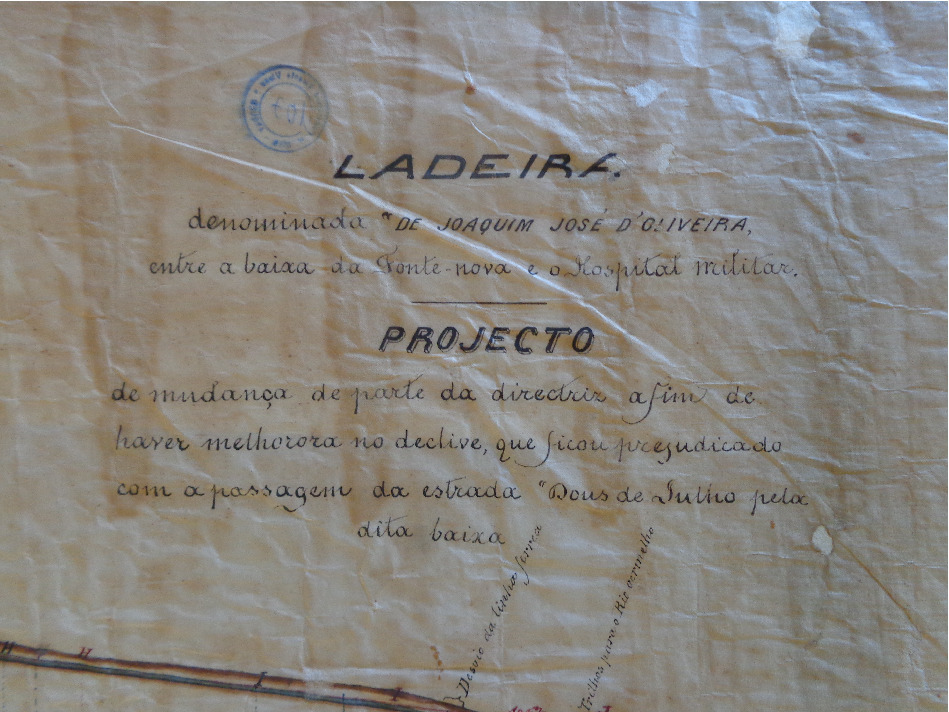
\includegraphics[width=0.4\textwidth]{3-cap2/complementos/mapas/joaquim/joaquim02.eps} 
\label{fig:joaquim02}
 }
\  %espaco separador
\subfloat[Data e autoria. \textbf{Fonte:} \textbf{BR BAAPB}, Biblioteca, planta 107]{
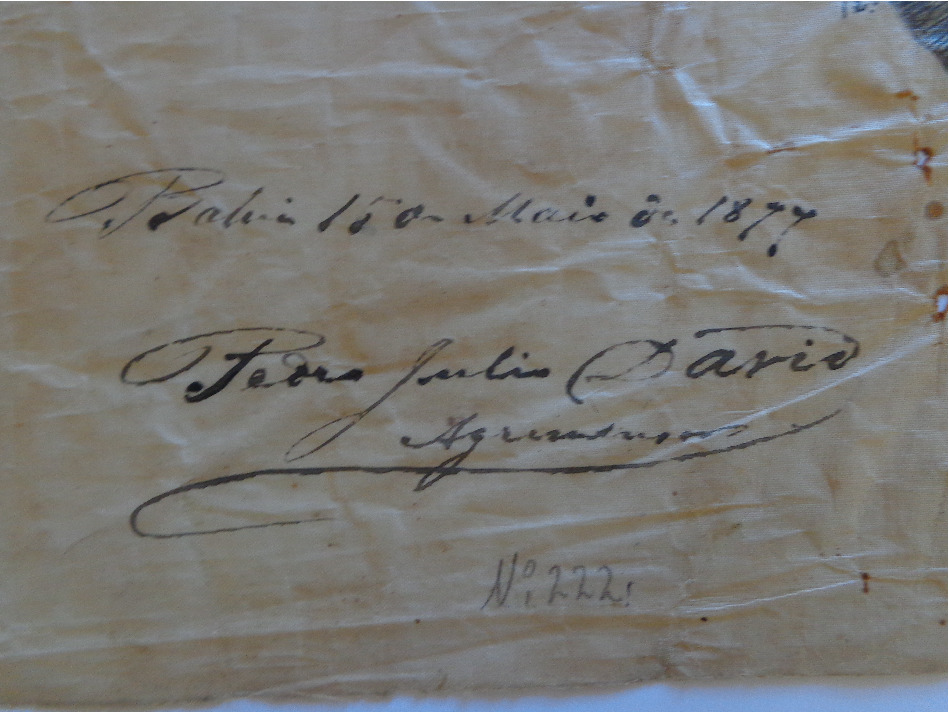
\includegraphics[width=0.4\textwidth]{3-cap2/complementos/mapas/joaquim/joaquim04.eps} 
\label{fig:joaquim04}
 }
\  %espaco separador
\subfloat[Planta da obra. \textbf{Fonte:} \textbf{BR BAAPB}, Biblioteca, planta 107]{
\includegraphics[width=\textwidth]{3-cap2/complementos/mapas/joaquim/joaquim01.eps} 
\label{fig:joaquim01}
 }
\caption{Projeto de mudança no declive da ladeira de José Joaquim de Oliveira, de autoria de Pedro Julio David (1877).}
\label{fig:joaquim}
\end{figure}

Outro aspecto notável, a ser visto em maiores detalhes na \autoref{subsec:pitangueiras} (p. \pageref{subsec:pitangueiras}) é que o palacete de Joaquim José de Oliveira foi adquirido pela província da Bahia em 1872 para a construção do \textit{Hospital Militar}, que ainda funciona no mesmo local depois de uma reforma completa realizada em 1953.

\subsection{Pitangueiras, Castro Neves, Sangradouro, Ladeira do Fabrício e Largo do Paranhos: urbanização acelerada e enobrecimento a pulso}\label{subsec:pitangueiras}

Durante o século XIX o chamado ``primeiro distrito'' de Brotas passava por transformações: as atividades agropecuárias e as herdades estavam sendo substituídas por palacetes, casas e pequenas chácaras de veraneio. Isto terá impacto direto sobre sua formação territorial e sobre o valor de sua terra no alvorecer da Primeira República, que finda o século. 

Embora o primeiro distrito de Brotas envolva a Boa Vista, a disparidade do processo de urbanização ocorrido nas localidades a seguir, quando comparadas com aquele verificado na Boa Vista, justificou separar esta última como sendo uma zona de transição entre  resíduo da ruralidade característica do segundo distrito da freguesia.

\subsubsection{Pitangueiras}\label{subsubsec:pitangueiras}

Passada a ladeira dos Galés, chega-se de imediato à estrada que os contemporâneos chamavam das \textit{Pitangueiras}, curto trecho entre o largo e a estrada do Matatu Pequeno, hoje conhecida como rua Barros Falcão. 

Já em 1858 o \textbf{Livro Eclesial de Registro de Terras da Freguesia de Brotas} registrava terras em nome do padre Felisardo Jerônimo Soares, a saber:

\begin{citacao}
O abaixo assignado possue na freguesia de Brotas e logar denominado Pitangueiras um terreno com sete braças de frente na mesma estrada de Brotas e cinco de fundo, que ficam na travessa, que vae da mesma estrada para a do Matatú, onde confina com terras de Francisco de Assis Gomes, confinando pelo lado do sul com terras do dito Assis, e do Capitam Salvador Pires de Carvalho e Albuquerque, tendo obtido este terreno por compra que fez a Marinha Rodrigues da Silva. Bahia, vinte e um de junho de mil oitocentos e cincoenta e oito. O Padre Felisardo Jerônimo Soares. E nada mais continhão as declarações [\textit{ilegível}] Brotas da Bª, 30 de junho de 1858. 
Vigº. Ernesto de Olivª Valle\footnote{\textbf{BR BAAPB}, fundo Colonial, série Registros de Terra, livro 4675, f. 16 verso.}
\end{citacao}

Outro proprietário de terras nas Pitangueiras era José Joaquim de Santa Tereza:

\begin{citacao}
Terra que comprou José Joaquim de Santa Tereza a Domingos José Cardozo no lugar denominado Pitangueiras, freguesia de Nossa Senhora de Brotas da Bahia, com tres braças de frente divide pelo norte com o próprio comprador pelo lado opposto com o Capitão Salvador Pery de Carvalho e pelo fundo com o padre Feliciano Jeronimo Soares. Brotas, dezesseis de julho de mil oitocentos e cincoenta e oito. José Joaquim de Santa Tereza. E nada mais continhão as declarações que me forão dadas. Brotas da Bª, 17 de julho de 1858\footnote{\textbf{BR BAAPB}, fundo Colonial, série Registros de Terra, livro 4675, f. 31 frente.}.
\end{citacao}

José Joaquim de Santa Tereza, falecido em 1889, teria sido muito provavelmente o mesmo ``crioulo forro, solteiro'', nascido em 1801, ``respeitável lavrador e comerciante residente em Brotas'' e ``aparentemente membro de candomblé'' que entre 1830 e 1831, no papel de comandante de um destacamento miliciano, afrontou seguidas vezes o juiz de paz de Brotas, Antonio Gomes de Abreu Guimarães \cite[pp.~54-59]{REISSILVA1989}. Chamou a atenção pelo fato de encontrarmo-lo, anos depois, em meio às licenças de construção e reforma do \textbf{Arquivo Histórico Municipal de Salvador}, embora já falecido, como ex-proprietário de um dos imóveis reformados, então de propriedade de seu legatário Roberto da Trindade de Jesus. Busca no \textbf{Arquivo Público da Bahia} revelou ainda existirem lá custodiados os autos de seu inventário, onde há fatos muito interessantes. Este senhor, rico porém analfabeto, ``catholico, apostolico romano [\dots] em a qual religião nasci e fui criado e educado e espero morrer para a salvação de minha alma'', além de deixar várias casas na rua do Cabral e na rua do Jogo do Carneiro (freguesia de Sant'Anna) para seu afilhado, parentes e escravos alforriados, outras tantas casas na rua da Paciência (Rio Vermelho) para seus amigos, quantias variadas para moradores da armação do Saraiva e de Itapuã e de deixar rendas e usufrutos para a Irmandade de Nossa Senhora do Santíssimo Sacramento e do Rosário de Brotas, legou a Izidra Prima de Jesus, irmã de seu afilhado Martiniano Primo de Jesus, uma casa térrea nas Pitangueiras, e a seu amigo Francisco Lopes Fiuza uma casa no largo de Brotas; descontados estes e uma grande quantidade de outros bens, rendas e pagamentos, e na ausência de herdeiros naturais, sobraram-lhe ainda bens suficientes para legar a Roberto da Trindade de Jesus, seu ``muito particular amigo'' e morador do largo de Brotas, como seu ``presumptivo e universal herdeiro'' e deixá-lo com uma relativa fortuna\footnote{\textbf{BR BAAPB}, fundo Judiciário, seção Inventários, estante 7, caixa 2989, documento 2.}. Em momento oportuno voltaremos a falar da fortuna deste herdeiro. 

Em 1863 Pitangueiras foi uma das localidades escolhidas para receber alguns dos 347 combustores de iluminação a gás que restavam para completar os 2 mil contratados com a presidência da província da Bahia \cite[p.~52]{bahia_rpe_1863}. Disto resultou um fato curioso: instalados os combustores, um indivíduo começou a apagá-los; preso e conduzido à presença do presidente da província, confessou que era acendedor de lampiões nas Pitangueiras e apagava-os por ordem do fiscal da empresa responsável pela iluminação pública assim que se mostravam ``amortecidos'', pois a multa cobrada pela polícia pelos amortecidos e pelos apagados era igual e os ``amortecidos'' -- ou seja, com iluminação fraca -- ainda consumiam gás \cite[relat.~chefe~polícia,~p.~25]{bahia_rpe_1870}. 

Em 1871 uma escola primária masculina havia sido recentemente removida para este povoado, medida elogiada pelo rápido crescimento das turmas e pela abertura de turmas noturnas para artistas-operários\footnote{\textbf{Jornal da Bahia}, ano XIX, nº 5.445, 21 set. 1871, p. 1.}; tal remoção, entretanto, teria prejudicado os moradores do largo de Brotas, que só em 1876, depois de muito peticionar ao governo provincial (ao que parece muito contente com a medida, pois registrou haver duplicado o número de alunos depois dela \cite[relat.~instrução~pública,~p.~25]{bahia_1872}), conseguiram deste a contratação de professores particulares para meninos e meninas da localidade\footnote{\textbf{O Monitor}, 03. set. 1876, p. 1.}. A situação, entretanto, ainda não havia melhorado em 1877, como se vê neste clamor assinado por um ``Amigo das Letras'':

\begin{citacao}
\textbf{Aos senhores deputados provinciaes}

Pedimos aos senhores deputados provinciaes que se dignem lançar suas vistas sobre a freguezia de Brotas desta capital, que muito necessita de duas escolas, sendo uma para cada sexo. As cadeiras dessa freguezia acham-se funcionando no logar denominado Pitangueiras -- de forma que um grande numero de crianças de um e outro sexo que moram no largo de Brotas e no Engenho Santo Antonio não podem receber a instrucção primaria.
Bahia, 18 de março de 1877\footnote{\textbf{O Monitor}, 22 mar. 1877, p. 3.}.
\end{citacao}

Ainda em abril de 1877 a situação da escola em Pitangueiras parecia periclitante, pois sua transferência para um extremo da freguesia resultara em grande evasão escolar\footnote{\textbf{O Monitor}, 28 abr. 1877, p. 1.}. Não é difícil deduzir desta situação que Pitangueiras era localidade de difícil acesso para os moradores do largo de Brotas e do Engenho Santo Antônio; pode-se igualmente deduzir, embora com menor certeza, a hipótese de que estas duas últimas localidades tivessem, entre 1871 e 1877, número de moradores maior que o de Pitangueiras. 

Há que se tomar cuidado com estas deduções; apesar das aparências, Pitangueiras era um dos polos pulsantes da urbanização de Brotas. Residiam nas Pitangueiras em 1872 Guilherme José da Costa, servente da Seção de Estatística da Secretaria da Presidência da província; Firmino Pacífico Duarte Gameleira, mesário do Hospital dos Lázaros; o capitão Maximiniano dos Santos Marques e José Carlos Ferreira, primeiro e quarto juízes de paz da freguesia de Brotas respectivamente; José Lourenço Ferreira Cajaty, diretor do Externato Normal; Manoel Luiz Gomes Vinhas, professor da escola pública de Brotas; José Diniz Gonçalves, partidor do Tribunal de Justiça; Sebastião José da Cruz Mello, segundo escriturário da Alfândega; Benjamin dos Santos Martins Vallasques, amanuense da Recebedoria \cite[segunda~parte, pp.~59, 85, 90, 91, 97, 98, 128, 167, 180]{pimenta_almanak_1872}. Funcionavam nas Pitangueiras as tavernas de Antonio Moreira da Silva, Domingos de Oliveira Bastos e Manoel José de Azevedo e Almeida; \cite[terceira~parte, pp.~40, 41, 48]{pimenta_almanak_1872}; o escritório de Francisco Antonio de Araujo, contratador de obras; e a oficina de encadernação de Herculano Antonio Leite\cite[quarta~parte, pp.~12, 39]{pimenta_almanak_1872}.

Já em 1879 Pitangueiras concentrava razoável infraestrutura urbana, pois anúncio de casa a alugar nesta localidade indicava ter a mesma ``os commodos necessarios para familia e encanamento de gaz''\footnote{\textbf{O Monitor}, 17 maio 1879, p. 2.}. Na mesma linha vai o anúncio de leiloamento dos seguintes imóveis, todos de bom padrão para a época:

\begin{citacao}
\textbf{Bens de raiz -- }Uma casa abarracada sita à rua das Pitangueiras, freguesia de Brotas, de n. 159, edificada em terreno proprio, com 8 metros e 10 centimetros de frente e 24 metros e 10 centimetros de fundo que dá para a rua Sete de Setembro, tendo de lado que dá para o beco 18 metros e 80 centimetros, com terraço na frente com gradil de ferro; a casa tem 2 janellas de peitoril e porta de vidraça no centro, 5 janellas do lado, sala de espera com porta para o becco, sala de visita, 2 quartos, salla de jantar e dispensa, e toda ella forrada, salla de gommar e cozinha, 3 quartos no quintal, lenheiro e sofás de cimento e concha para recreio, quintal todo murado com um portão para a dita rua, sotão com sala e 3 quartos, paredes todas dobradas, divide-se por um lado com casa do mesmo casal, avaliada por 4:000\$000.

Uma casa abarracada sita na dita rua e freguezia, de n. 157, edificada em terreno proprio, com 7 metros e 80 centimetros de frente com terraço e gradaria de ferro, com 2 janellas e porta no centro, sala de frente, 3 quartos, sala de jantar e toda ella forrada, dispensa, cozinha, sala de gommar com 2 quartos no quintal, sotão com janellas para a frente e fundo, com sala e 3 quartos, quintal todo murado com porteira para a rua Sete de Setembro, divide-se a casa por outro lado com casa do casal, avaliada por 3:000\$000.

Um terreno sito à rua Sete de Setembro, na dita freguezia, tendo de comprimento 38 metros, dividindo-se pelo fundo com terrenos do Hospital Militar, tendo diversas casas n'elle edificadas, avaliado cada metro por 15\$000 e todos por 570\$000 [\dots]\footnote{\textbf{O Monitor},3 out. 1879, p. 2.}.
\end{citacao}

O \textit{intérieur} das habitações das Pitangueiras era rico e bem ornamentado, como se pode ver a partir deste anúncio:

\begin{citacao}
Leilões [\dots]

Luiz Zuanny 

Venderá em leilão na terça-feira 2 de dezembro (dia desoccupado) às 11 horas em ponto na chácara as Pitangueiras, estrada do Matatú, freguezia de Brotas, por conta de quem pertencer, o seguinte: mobília de jacarandá, dita de Gonçalo Alves, mobilias autriacas, um piano de Pleyel n. 4 quasi novo, tapetes, escarradeiras, jarras finas de Bacarat, figura de Biscuit, quadros a oleo, espelho com grande moldura dourada, ditos pequenos, um lustre de cristal de 6 luzes, ditos de 3 e 2 luzes, arandellas de cristal e metal, tudo para gaz, cantoneiras, venesianas, pannos de crochet e de renda para cadeiras, etc., uma importante mobilia de quarto de Gonçalo Alves a Luiz XV, composta de cama, toilete e lavatorio, retrete e dous guarda-vestidos, uma pequena mobilia de Gonçalo Alves para gabinete, sendo o sofá e 8 cadeiras a Luiz XV obra moderna, cortinado de crochet para cama, cantoneiras com pedra marmore, uma grande mesa de vinhatico para jantar, guarda-louças, com etagéres, quartinheiro, guarda-comidas, cadeiras de vinhatico, dita de vimes, apparelho de porcellana para jantar, dito para almoço, copos, calices, garrafas, compoteiras, fructeiras, bandeijas, trem de cosinha, etc., etc., etc.

\textbf{Attenção}

No mesmo dia às 2 horas da tarde se vendera a importante chácara com excelente casa de morada e dependencias, grande jardim com gradil de ferro, brejo, plantação de capim e porção de arvoredos fructíferos etc.\footnote{\textbf{Gazeta da Bahia}, ano I, nº 267, 25 nov. 1879, p. 2}.
\end{citacao}

Considerava-se situado nas Pitangueiras o ``predio nobre'' pertencente aos herdeiros do coronel Antonio José de Lima, comprado pelo Ministério da Guerra em 1872 para a instalação do \textit{Hospital Militar} \cite[p.~30]{bahia_1872}, ainda hoje existente na ladeira dos Galés (embora o ``prédio nobre'' tenha sido demolido em 1953) (cf. \autoref{fig:hospmil}, p. \pageref{fig:hospmil}). Tratava-se do antigo palacete de Joaquim José de Oliveira \cite[p.~36]{bahia_rpe_1874}, que por caminhos comerciais ou sucessórios fora parar em mãos de Antonio José de Lima, depois de seus herdeiros e por último com a província. A aquisição, um investimento de 70:000\$000 \cite[p.~10]{bahia_1872}, foi saudada por estarem ``attendidas as condições essenciaes de um bom hospital'': ``vastidão, solidez, bella e saudavel situação, proximidade do interior da cidade, servido pela linha de \textit{Trilhos Centraes} e em um bairro muito procurado'' \cite[p.~31]{bahia_1872}.

\begin{figure}[!htp]
\centering
\subfloat[O ``prédio nobre'' em 1872. (\textbf{Fonte:} www.hges.eb.mil.br)]{
\includegraphics[width=1\textwidth]{3-cap2/complementos/imagens/1872-hospitalmilitar[www.hges.eb.mil.br].eps}
\label{fig:hospmil1872}
 }
\  %espaco separador
\subfloat[Prédio atual, datado de 1953. (\textbf{Fonte:} www.hges.eb.mil.br)]{
\includegraphics[width=1\textwidth]{3-cap2/complementos/imagens/1953-hospitalmilitar[www.hges.eb.mil.br].eps} 
\label{fig:hospmil1953}
 }
\caption{Hospital Militar de Salvador em dois tempos}
\label{fig:hospmil}
\end{figure}

A situação topográfica das Pitangueiras, na cumeada de uma elevação, assim como a passagem dos bondes por toda sua extensão, devem ser levadas em conta como fatores de valorização da terra na localidade.

\subsubsection{Castro Neves}\label{subsubsec:castroneves}

Um setor específico de Brotas veio a destacar-se com o tempo: o \textit{Castro Neves}, situado nas faldas da cumeada das Pitangueiras, entre elas e o Sangradouro.

\textit{Manoel de Castro Neves}, contemporâneo de Joaquim José de Oliveira, era rico comerciante português com atuação em Salvador, que chegou inclusive a subvencionar tropas favoráveis à independência do Brasil\footnote{\textbf{Idade D'Ouro do Brazil}, várias edições entre 1811 e 1823; \textbf{Correio Mercantil}, vol. III, nº 587, 24 out. 1838, p. 4; \textbf{Correio Mercantil}, ano VI, nº 194, 13 set. 1839, p. 4.; \textbf{Correio Mercantil}, ano. VII, nº 270, 16 dez. 1840, p. 4; \textbf{Correio Mercantil}, ano VII, nº 272, 18 dez. 1840, p. 4; \textbf{Correio Mercantil}, ano VIII, nº 97, 10 maio 1841, p. 4; \textbf{Correio Mercantil}, ano VIII, nº 98, 11 maio 1841, p. 4;  \textbf{Correio Mercantil}, ano VIII, nº 108, 24 maio 1841, p. 4; \textbf{Correio Mercantil}, ano VIII, nº 183, 30 ago. 1841, p. 4;}. A documentação pesquisada e a bibliografia consultada indicam que este comerciante português era dono de terras contíguas às de Joaquim José de Oliveira, embora não tenha sido possível descobrir a extensão de seu patrimônio ou seus limites precisos. Sabe-se pelas mesmas fontes, entretanto, que parte significativa da urbanização da localidade se deu sobre terras foreiras a seus herdeiros, como o alferes Henrique de Castro Neves, residente às Pitangueiras até 1873, quando foi transferido para o Rio de Janeiro\footnote{\textbf{Almanak Administrativo, Mercantil e Industrial da Bahia} de Camilo Masson, várias edições entre 1854 e 1863.}. 

Já em 1863 havia uma ``r. de Castro Neves'' onde residia funcionário público Nicolau Tolentino de Brito Caraúna \cite[p.~125]{masson_almanak_1863}. Em 1872 residiam nesta mesma rua o bedel José Viríssimo de Almeida, da Faculdade de Medicina; o professor de álgebra e aritmética Firmino Pacífico Duarte Gameleira; o carteiro Joaquim Maria Soares, da Tesouraria da Fazenda; Olegario Feliciano de Castilho, fiel de armazém da Alfândega; Cypriano Theodoro Pereira de Mello, agente de trapiche da Alfândega; Manoel Francisco Leite, fiscal exterior da Mesa de Rendas Provinciais; e Joaquim Mariano Pinto Bezerra, porteiro do Arsenal de Guerra \cite[segunda~parte, pp.~94, 96, 167, 170, 184, 194]{pimenta_almanak_1872}. Funcionavam no Castro Neves também em 1872 a taverna de Dalia Roza da Silveira e o açougue de Ritta Freire de Sant'Anna \cite[terceira~parte, pp.~41, 54]{pimenta_almanak_1872}; o ponto de aluguel de carroças de João Gonçalves Mamede, a oficina do latoeiro João José Barbosa, a litografia de João Rodrigues da Silva e as tipografias de João Emygdio da Silva Lima e Luiz Antônio Pereira da Silva \cite[quarta parte, pp.~20, 32, 36, 38]{pimenta_almanak_1872}. Se considerarmos a \textit{rua do Socorro} (atual rua Arlindo Fragoso) como integrante do Castro Neves, é preciso adicionar à localidade a tipografia de Otylio Olympio de Andrade Faria e as oficinas de encadernação de Felix Antonio Possidonio e Manoel Theodoro da Silva \cite[quarta parte, pp.~38, 39]{pimenta_almanak_1872}. Como a \textit{ladeira dos Galés} é um dos limites do Castro Neves, é preciso incluir nesta contagem a barraca de cereais de Domingos de Oliveira Bastos e a taverna e o açougue de Antonio Meirelles da Silva \cite[terceira~parte, pp.~39, 53, 56]{pimenta_almanak_1872}.

Funcionários públicos afluíam para a localidade e tomavam-na como residência, indicando ter ela elementos de interesse para gestores de médio e baixo escalão, bem acima da média em termos de renda pessoal. Estariam eles atrás da valorização imobiliária promovida pela instalação do Hospital Militar e da infraestrutura urbana instalada na área, como a linha dos Trilhos Centrais? Ou seriam, eles próprios, os agentes desta valorização e da implementação de infraestruturas? As duas hipóteses parecem conjugar-se. De um lado, já se viu na \autoref{subsec:josejoaquim} como a ladeira dos Galés foi consertada em 1877 (\autoref{fig:joaquim}, p. \pageref{fig:joaquim}) muito em função do acesso ao Hospital Militar, resultando em valorização do local. De outro lado, o afluxo de funcionários públicos à localidade tinha efeitos quase imediatos: foi este funcionalismo público, somado aos terratenentes locais (os herdeiros de Manoel de Castro Neves), quem exerceu pressão sobre a administração municipal e provincial em busca da instalação de infraestrutura e serviços urbanos na área; sua instalação resultava não apenas em melhor qualidade de vida para os habitantes, mas também em valorização imobiliária. 

Em 1876 uma reclamação contra o ``descuido policial'' dizia ser o Castro Neves ``quarteirão populoso'', mas que, ``privado dos beneficios da illuminação publica'', prestava-se a ``ser um ponto onde se perpetre, apatrocinado pelas trevas, mais de um crime''\footnote{\textbf{O Monitor}, ano I, nº 81, 10 set. 1876, p. 1}. Em 1880 a edilidade e a administração provincial eram admoeastadas a cuidar do Castro Neves, localidade tornada ``refugio de fascinorosos e balcão das mais torpes imoralidades'' por força da falta de iluminação e da falta de calçamento que a deixava ``totalmente intransitável'' no inverno, ``prejudicando os interesses de quem ali habita''\footnote{\textbf{A Gargalhada}, nº 8, 1880, p. 2}. Cinco combustores foram instalados na rua do Socorro para a iluminação pública em 1872 \cite[relat.~obras~públ.,~p.~38]{bahia_1872}, mas em 1º de junho de 1881 um morador do Castro Neves oficiou à Assembleia Legislativa provincial pedindo a instalação de ainda mais combustores para iluminação pública na localidade \cite[p.~3]{bahia_relatassleg_1881}. Em 3 de fevereiro de 1889 vinha a público reclamação contra uma criação de porcos no Castro Neves, a quem se atribuía a causa da grande escala de casos de febre no local\footnote{\textbf{Diário do Povo}, nº 218, 03 fev. 1889, p. 1}; a reclamação parece ter surtido efeito, pois no expediente de 5 de agosto de 1889 a Câmara Municipal autorizou o investimento de 150\$000 no ``melhoramento da rua do Socorro ao Castro Neves e bem assim da estrada da Boa Vista''\footnote{\textbf{Diário da Bahia}, ano XXXV, nº 245, 01 nov. 1889, p. 2}, e em 14 de agosto o inspetor de obras Alcebiades Demetrio de Barros Palacio pedia a liberação de 33\$500 para comprar as ferramentas necessárias ao início da empreitada\footnote{\textbf{Diário da Bahia}, ano XXXV, nº 247, 5 nov. 1889, p. 1.}.

A valorização imobiliária corria em paralelo às pressões pela implementação de infraestruturas urbanas. Já em 1872 encontramos anúncio de ``bom rendimento com segurança'', consistindo em venda do ``direito senhorio de 343 braças de terrenos aforados a diversos'' no Castro Neves, ``cujos foros são de rs. 690\$ alem do laudemio''\footnote{\textbf{Correio da Bahia}, ano II, nº 27, 27 abr. 1872, p. 4}. Em 24 de abril de 1877 Félix Francisco oficiou à Câmara Municipal solicitando permissão para construir em seu terreno\footnote{\textbf{Correio da Bahia}, ano VII, nº 33, 04 maio 1877, p. 2}. José Braz Nepomuceno seguiu-se a ele, requerendo em 25 de abril de 1878 aforamento de terrenos baldios pertencentes ao Hospital Militar\footnote{\textbf{O Monitor}, ano II, nº 280, 9 maio 1878, p. 1}. A disputa por terra no Castro Neves era acirrada: em 3 de outubro de 1883 o comendador Joaquim Teixeira Chaves publicava anúncio na imprensa prevenindo que 

\begin{citacao}
ninguém arremate 20 braças de terra sita à rua Direita do Castro Neves [\dots] que se acha em praça pelo juizo de orphãos, e cartorio do escrivão Garcia, como pertencente ao espolio do intestado Cazimiro Coelho Sampaio, visto que são do dominio do annunciante, e assim tem protestado mostrar pelo competente juizo\footnote{\textbf{Diário de Notícias}, ano 7, nº 223, 03 out. 1881, p. 2}.
\end{citacao}

Não espanta que a terra no Castro Neves fosse assim disputada às vistas do público, pois as casas no Castro Neves eram muito bem constituídas, como se vê por este exemplo retirado do leiloamento da propriedade de Firmo Lopo da Silva:

\begin{citacao}
Uma casa térrea sita à rua do Castro Neves, freguezia de Brotas, sem numero, com 3 janellas envidraçadas e porta de entrada do lado, com 6 ms. e 30 cents. de frente, tendo n'este um gradil de ferro com portão, e jardim ao lado; tem sala e alcova forrada e cimentada, 2 quartos cimentados, sala de jantar e cosinha fóra assoalhados, e estes com os de telha vã, grande quintal com arvoredos fructiferos. Devide por um lado com a casa de Jeronymo de tal, e pelo outro com quem de direito tiver. As paredes da caixa da propriedade são dobradas e proprias, e as mais singellas; é edificada em terreno foreiro aos herdeiros de Castro Neves, a qual propriedade deverá ser arrematada por quem maior lance offerecer sobre sua avaliação que é de rs. 1:500\$000 [\dots]\footnote{\textbf{Gazeta da Bahia}, ano IV, nº 207, 14 set. 1882, p. 2}.
\end{citacao}

Mesmo as casas menores pareciam muito sedutoras para o mercado imobiliário da época, como se vê neste anúncio:

\begin{citacao}
\textbf{Vende-se}

Pela quantia de 700\$000, uma casa fabricada de novo a rua do Socorro do Castro Neves, com porta e janella alta e moderna, sala de jantar, cosinha fora, seu pateo com todos os despejos, e grande quintal posterior de renda actual de 1\$000 mensaes.

A tratar com o major Benjamin Matheus dos Santos, junto do Forum\footnote{\textbf{Gazeta da Bahia}, ano V, nº 64, 25 mar. 1883, p. 2}.
\end{citacao}

Não é de espantar, num tal quadro, que o Castro Neves fosse ponto concorrido dos festejos do Dois de Julho:

\begin{citacao}
\textbf{Bando}

No domingo 22 do corrente, às 3 horas da tarde, terá logar o bando annunciador dos festejos do Dous de Julho do \textit{Castro Neves}, que reunindo-se no largo do mesmo nome, percorrerá as ruas seguintes: Alegria, Sangradouro, Socorro, ladeira dos Galés, 25 de Março, largo dos Milagres, becco do Padre Felizardo e Boa-Vista, onde se dispersará\footnote{\textbf{Gazeta da Bahia}, ano V, nº 163, 22 jul. 1883, p. 2}.
\end{citacao}

Como se verá em momento adequado, o Castro Neves chegará à República em 1889 como uma curiosa área residencial onde palacetes confrontavam-se com estábulos e roças.

\subsubsection{Sangradouro}\label{subsubsec:sangradouro}

Outro ponto onde os processos de valorização imobiliária mostravam-se com toda força era o \textit{Sangradouro}. Curiosamente, o Sangradouro, por onde corria um rio\footnote{\textbf{Correio da Bahia}, ano VI, nº 257, 09 fev. 1877, p. 3} (daí, muito provavelmente, seu nome), havia sido no primeiro terço do século XIX lugar perigoso, infestado de ``salteadores''.

Residiam no Sangradouro em 1845 o major Joaquim Olavo da Silva Rabello, do 1º Batalhão de Caçadores, que também trabalhava como ajudante da Alfândega \cite[pp. 302, 367]{almanach_1845}; trata-se do único funcionário público citado pelo \textbf{Almanach} de 1845 a residir na localidade. A situação, entretanto, mudava a partir de 1855: já se contavam como residentes da localidade Antonio José Teixeira Júnior, amanuense da Tesouraria da Fazenda mencionado no \textbf{Livro Eclesial de Registro de Terras da Freguesia de Brotas} como um dos proprietários de terras na área\footnote{\textbf{BR BAAPB}, fundo Colonial, série Registros de Terra, livro 4675, f. 15 frente.}, e o agora tenente-coronel do 2º batalhão da reserva Joaquim Olavo da Silva Rebello, que além de ajudante do escrivão da entrada e descarga da Alfândega acumulou também o cargo de subdelegado de polícia da freguesia \cite[pp.~173, 176, 212]{masson_almanak_1855}; instalou-se na localidade no ano seguinte o amanuense da Alfândega e inspetor de quarteirão Jorge Luiz Schwind Avellos \cite[pp.~155, 248]{masson_almanak_1856}; em 1857 foi a vez de chegarem à localidade Fabrício Alves de Araújo e Almeida, terceiro escriturário da Contadoria da Tesouraria Geral da província, que aparecerá com destaque na \autoref{subsubsec:fabricio} (p. \pageref{subsubsec:fabricio}), e Manuel Joaquim Garcia, amanuense da 1ª seção da Repartição de Polícia \cite[p.~163, 242]{masson_almanak_1857}. Chegaram também ao Sangradouro, em 1860, o tenente Manuel Agostinho da Cruz e Mello; Francisco Lazaro da Cunha Bacellar, escriturário da Caixa de Economias; o guarda-livros João Pires Moreira; e os músicos Manuel Emilio Pereira Bião, Manuel Pereira Bião e Manuel Pereira Bião Filho  \cite[p.~222, 311, 344, 350]{masson_almanak_1860}. Em 1862 o número de residentes no Sangradouro multiplicou-se\footnote{Como a publicação nos almanaques era paga, não se pode afirmar com segurança, tendo-os como única fonte sobre o assunto, se o que houve foi um aumento da população na localidade, com causas a investigar, ou se se tratou somente de maior disponibilidade de anunciantes. A sequência da exposição desta pesquisa, entretanto, mostrará um aumento no número de anunciantes no almanaque de outra gráfica, tanto em sua quantidade quanto em sua diversidade.}: além dos moradores já mencionados, são relacionados também Domingos de Faria Macedo, diretor no Instituto Dramático; o músico Joaquim Cornelio de Santa Anna Torres; registrava-se, além disso, o funcionamento da taverna de Manuel de Jesus Neves \cite[p.~305, 324, 394]{masson_almanak_1862}.

Em 1872 residiam na localidade os oficiais de justiça Umbelino José da Costa e João Gonçalves da Silva; Joaquim Olavo da Silva Rabello, o militar já conhecido como escriturário da Alfândega; \cite[segunda~parte, pp.~60, 128, 167]{pimenta_almanak_1872}; além disso, existiam as tavernas de João José Inocêncio de Barros e Ricardo Augusto da Silva Godinho \cite[terceira parte, pp.~43, 49]{pimenta_almanak_1872}; a padaria de João Antonio Dias Guimarães \cite[terceira parte, p.~52]{pimenta_almanak_1872}; o escritório do advogado Manoel José dos Reis, o ponto de aluguel de carroças de Germano José do Sacramento Baraúna, o ateliê do escultor Luis Hermogenes Victorino Pereira, as oficinas dos litógrafos Antonio de Oliveira Bottas e Florentino de Oliveira Dias, a tipografia de José Neville da Cunha Mello e a oficina do fogueteiro Saturnino Vieira de Carvalho Macedo \cite[quarta parte, pp.~2, 20, 35, 36, 38 43]{pimenta_almanak_1872}. Anúncio na imprensa anunciava que Job de Carvalho, médico especialista em ``molestias syphiliticas'', atendia em seu consultório de meio dia em diante, mas atendia a qualquer hora em sua casa na rua do Sangradouro\footnote{\textbf{O Monitor}, ano V, nº 229, 17 mar. 1881, p. 2}. Em 1888 somavam-se a estes residentes Felippe Candido Moreira, segundo oficial do Tesouro Provincial; e Pedro Americo Tupy, auxiliar da Polícia do Porto \cite[pp.~18, 30]{carvalho_almanach_1888}. 

Um exemplo do tipo de moradias existentes no Sangradouro no último terço do século XIX:

\begin{citacao}
\textbf{Leilão}
De uma chácara ao Sangradouro, estrada nova, por onde passam os \textit{wagons} da linha Central.
LUIZ ZUANNY -- venderá em leilão na terça-feira 20 do corrente, ao meio dia, uma chácara no Alto do Sangradouro, com entrada pela ladeira que parte da rua que segue das Sete Portas para a Fonte Nova, passagem dos wagons da linha Central; com boa casa de morada, muito fresca, e excelente vista, tendo terraços dos lados com grades de ferro, jardins, um bom pomar, muitos arvoredos fructiferos, portão de ferro na frente e terreno para plantações [\dots]\footnote{\textbf{Jornal da Bahia}, ano XIX, nº 5.565, 15 fev. 1872, p. 3.}.
\end{citacao}

Outro exemplo, num anúncio de 1877:

\begin{citacao}
Perante este juízo na terceira praça, que ha de ter logar na porta do Forum, no dia 10 de dezembro proximo futuro, terão de ser vendidos: -- o sobrado grande, com grades de ferro na frente do jardim, com duas grandes lojas, de um andar, e sotão, construida de pedra e cal toda a caixa, sito em terreno proprio á rua do Sangradouro, freguesia de Brotas, e quasi defronte das casas do Sr. Antonio Francisco Ribeiro Guimarães, tendo por base o preço de seis contos de reis [\dots]\footnote{\textbf{O Monitor}, ano II, nº 147, 25 nov. 1877, p. 2}
\end{citacao}

Ainda outro exemplo, de 1878:

\begin{citacao}
\textbf{CASA A VENDA}
Na ladeira da Glória, no Sangradouro, d'esta cidade, vende-se uma excellente casa abarracada, com 4 janellas de frente, entrada lateral, ha pouco edificada, com um grande quintal alguns arvoredos; quem a quizer vêr póde procurar as chaves em poder de sua proprietaria, na rocinha junto, do filho do finado Umbelino José da Costa, e para tratar á ladeira da Praça n. 19\footnote{\textbf{O Monitor}, ano III, nº 122, 27 out. 1878, p. 2}
\end{citacao}

Um último exemplo, de 1881:

\begin{citacao}
Correm praças nos dias 12, 15 e 19 do corrente mez ao meio dia, na porta do Forum, depois da audiencia, para serem arrematadas por quem mais der dinheiro a vista na 3ª praça, pagando os impostos de lei, as propriedades seguintes, pertencentes ao falecido João Antonio Mourão: [\dots] casa à rua do Sangradouro, freguezia de Brotas, à rua da Alegria, em terreno proprio, com 5m e 50 cent., com terreno ao lado da casa, n'esta 3 janellas e porta para o lado, grande quintal ou ribanceira, edificado sobre pilares e paredes singelas, com 11 pés de larangeiras no quintal, divide-se pelo sul com Henrique Francisco de Oliveira, e norte com Boaventura: avaliada por 2:000\$\footnote{\textbf{O Monitor}, ano VI, nº 28, 09 jul. 1881, p. 2}.
\end{citacao}

O mesmo anúncio apregoava uma casa ``em terreno proprio com 3m e 50 cent. de frente, com terreno ao lado, grande quintal'', também do falecido João Antonio Mourão, avaliada 500\$000.

Ocorre que entre os moradores do Sangradouro nem sempre encontravam-se os ``respeitáveis'': anúncio na imprensa chamava atenção para ``um réo de policia de nome Mascarenhas, que reside para os lados do Sangradouro'', que teria entrado na casa de certa Amelia, moradora de uma das casas do Barão da Palma, e levou três anéis de valor, além de haver ``assaltado a diversos quintaes em alta noite e dado completa busca'' e de andar sempre armado\footnote{\textbf{O Monitor}, ano III, nº 127, 03 nov. 1878, p. 2}.

Vê-se assim processo similar ao ocorrido no Castro Neves. Difere deste, não obstante, pois os imóveis encontrados na documentação pesquisada têm um quê de rurais, algo entre a casa de morar e a chácara, a habitação e a casa de campo. Outra diferença é a completa ausência de quaisquer movimentações dos moradores em prol da instalação de infraestruturas urbanas; se houve, certamente os moradores do Castro Neves foram mais estridentes e ocuparam os espaços disponíveis na imprensa muito mais assiduamente. 

\subsubsection{Ladeira do Fabrício}\label{subsubsec:fabricio}

Por ser de 1851, o mapa de Weyll ainda não poderia mostrar a \textit{ladeira do Fabrício}, conhecida a princípio como \textit{estrada do Sangradouro ao Matatu}, que corresponde ao trecho que inicia na atual rua dos Tupys, esquina com a atual rua do Sangradouro, e segue pela atual ladeira dos Bandeirantes até encontrar-se com a estrada para o Matatu no local onde hoje a ladeira dos Bandeirantes faz encruzilhada com as atuais ruas Alberto Torres, Barros Falcão e Amazonas. 

Esta ladeira foi mandada abrir em 1876 pelo governo provincial, em obras supervisionadas por uma comissão ``composta do Tenente-Coronel Fabricio Alves de Araujo, Bacharel Firmino Duarte Pacifico Gameleira e Negociante Manuel da Silva Pereira Guimarães'' \cite[p.~23]{bahia_1878}. A obra já se encontrava concluída no ano seguinte, sendo alargada de seus 8,8m originais para a largura de 11m e tendo recebido na mesma ocasião ``declives menos fortes'' \cite[p.~228]{bahia_1879}, e em 1885 recebeu calçamento \cite[p.~11]{bahia_1885}. É deste tenente-coronel que a ladeira veio a receber o nome.

Não foi encontrada na documentação pesquisada ou na bibliografia consultada qualquer referência a moradores da localidade, a escritõrios, consultórios ou oficinas, ou mesmo à implementação de infrastruturas urbanas; é razoável crer, dada a acentuada inclinação da ladeira, que tenha permanecido inabitada no último terço do século XIX, e que assim tenha chegado à República, quando encontrá-la-emos como sítio de algumas das mais interessantes obras residenciais do período.

\subsubsection{Largo do Paranhos}\label{subsubsec:paranhos}

A porta de entrada para o Matatu, no sentido de quem vem da ladeira dos Galés, é o \textit{largo do Paranhos}, assim batizado, ao contrário do que parece, não em homenagem ao já mencionado latifundiário Tomás da Silva Paranhos (cf. \autoref{subsec:nisa}, p. \pageref{subsec:nisa}), mas em homenagem a seu filho homônimo, que por décadas residiu no local \cite{dorea_ruas_1999}.

Embora se trate de localidade muito pequena, certamente passível de agrupamento no Matatu ou nas Pitangueiras, sua situação num entroncamento viário justifica seu destaque.

Exatamente as características privilegiadas de sua situação fizeram do largo do Paranhos uma localiade bem valorizada. Observe-se com detalhe a estrutura e o valor de um imóvel anunciado para o leiloamento: trata-se de uma roça de propriedade de Herman e Sophia Both, penhorada pela Sociedade de Commercio, descrita no anúncio a seguir:

\begin{citacao}
Uma roça em terreno proprio, na freguezia de Brotas, largo denominado de Paranhos, tendo a frente para o mesmo largo, dividindo-se pelo lado direito com a roça que foi do Bacharel Firmino Duarte Gameleira; pelo esquerdo, com a estrada que vai para a Quinta das Beatas; e pelo lado direito continuando de fundo à frente com terreno que foi do dito Bacharel Gameleira onde vae acabar. Medida a frente da roça, acha-se n'ella 336m 10c; do canto que vira para a estrada da Quinta das Beatas até encostar na roça que foi do Bacharel Gameleira, havendo n'este lado 143m 60c; de terreno, com o fundo de 43m 25c, que foram dados por aforamento a diversos, pelos executados, de modo que fica a frente propriamente dita da roça com 180m 50c, desde o terreno aforado até a esquina para a estrada das Boiadas, e essa frente está fechada por muros de boa construcção, tendo um portão de ferro por onde é a entrada principal para a roça e casa de morada. A entrada do portão para a casa é guarnecida de perfeitas cercas de pitangueiras, que terminam em 2 carramanchões sobre pilastras de pedra de cantaria; dentro das cercas de pitangueiras existem diversas arvores, como saputizeiros, abacateiros, laranjeiras etc., havendo no lado esquerdo da mesma roça diversas divisões formadas por cercas de pitangueiras, e em todos esses lotes diversas arvores, como as declaradas, cuja quantidade é a seguinte:

Na parte cultivada da roça existem: 60 jaqueiras, 73 mangueiras, 193 laranjeiras, 10 pes de fructa pão, 8 cajazeiras, 8 abacateiros, 24 saputizeiros, 23 coqueiros, 2 genipapeiros, 1 tamarindeiro, 4 [ilegível] de parreira, sendo algumas de pés direitos de cantaria, 1 brejo que termina em uma ribanceira, onde existe uma capoeira para corte de madeira, 1 telheiro fechado por paredes de taboas com uma machina à vapor em bom estado, serve para conduzir agua a um deposito junto á propriedade da morada, a qual agua é puxada por um encanamento de ferro, de um deposito de pedra e cal cimentado e coberto tambem com telheiro, 1 banheiro fechado por paredes de pedra e cal, e coberto de telhas, com 2 portas e 3 torneiras de bronze.

Uma casa de campo de gosto antigo com varandas fechadas por frontoes, e n'elles peitoris, tendo no lado direito da varanda, 1 oratorio de celebrar missa. A entrada é por uma porta entre 4 janelas, com sala aberta que occupa a porta e 2 janelas, e 1 gabinete em cada lado, tendo cada gabinete 1 janella, e a entrada para o interior da casa é pela sala de jantar que dá em 1 salão, havendo de cada lado deste 1 corredor, com diversos repartimentos que são: 10 quartos, dispensa e cozinha, toda construida de pedra e cal e de gosto antigo. Depois desses repartimentos um grande salão de pedra e cal, com paredes dobradas, feito muito depois da casa, e de gosto moderno, rodeado de janellas de vidraças, isto é, com janelas de vidraças no fundo e no lado, e a parte por onde abre-se para um terraço d'onde desce-se para o centro da roça por uma escada de pedra, sobre este salão há um sotão para onde sobe-se por uma escada interna, tendo o mesmo sotão 4 divisões eguaes (4 grandes quartos ou 4 pequenas salas) cada uma com 2 janelas de vidraças, pelo que é o dito sotão rodeado de janellas, tanto a sala da frente como os quartos e o salão são forrados; a sala e os mais commodos terreos são cimentados, e o sotão é de lages de pedra; a casa descripta e o seu acrescimo (salão e sotão) tem de frente 12m60c de comprimento de frente a fundo 38m30c, cinco senzalas cobertas de telha em estado de reparo, dentro da roça, com 25m90c de frente; e em seguimento as mesmas senzalas 2 cazinhas que estão alugadas, e cujos inquilinos aproveitam-se na entrada e sahida do porão da cocheira.

Em frente ás senzalas e encostado ao muro da roça, existe um grande armazem, onde foi antiga estribaria, que ainda hoje tem em parte mangedouras, armazem esse que é coberto de telhas e precisa de reparos. A roça, casa e mais dependencias as avaliaram em 10:000\$000 [\dots]\footnote{\textbf{O Monitor}, 10 dez. 1879, p. 2.}.
\end{citacao}

Trata-se de fazenda bem constituída, de gente abastada o suficiente para ter inquilinos; rural como seja, seu perfil enquadra-se em categoria semelhante às vizinhanças em urbanização ao redor.

\subsection{A fazenda Boa Vista e seus arredores: transição entre rural e urbano}\label{subsec:boavista}

A área circunvizinha ao solar Boa Vista correspondia à herdade de mesmo nome, a \textit{fazenda Boa Vista}. Parte da história desta área já foi vista na \autoref{subsec:pontciv} (p. \pageref{subsec:pontciv}); curiosamente, \textit{nenhum} dos proprietários mencionados naquela curta notícia histórica é mencionado no \textbf{Livro Eclesial de Registro de Terras da Freguesia de Brotas}, sequer o médico Antônio José Alves, de quem seria de se esperar, por força da imposição do ``registro do vigário'' pela Lei 601/1850, que ao comprar o solar em 1858 corresse para registrar sua propriedade junto ao pároco da freguesia. O mais provável, entretanto, é que as terras da Boa Vista não fossem oriundas de sesmarias, mas sim privadas, o que ao mesmo tempo teria dispensado o ``registro do vigário'' e redirecionado seu registro a um cartório; por ultrapassar o escopo da pesquisa em exposição, e por implicar em custas cartorárias proibitivas, não será pesquisada a cadeia sucessória dos proprietários deste imóvel. A descrição mais precisa encontrada na bibliografia pesquisada, ainda sem atribuição da titularidade da posse ou propriedade, foi aquela de um alvará: 

\begin{citacao}
Uma propriedade nobre e de sobrado, sita na Fazenda ‘Bôa Vista’ na Estrada de Brotas, freguesia do mesmo nome, em terreno proprio, com cento e quatro palmos de frente, e cento e trinta e cinco de fundo, tem na sua entrada grande portão de ferro, com proporções para um jardim; no pavimento terreo tem duas salas de frente, sete grandes quartos, um grande salão que comprehende todo o fundo, grande cozinha, tem bôa capella dourada, com Imagens, paineis e mais utensilios; no segundo pavimento, sala de entrada, duas salas de frente, no fundo tres salas, tres grandes quartos e dous menores, tem grande mirante dividido em tres partes com grandes salões e toda de paredes dobradas e as divisões de frontaes singelos, avaliada em trinta e oito contos de réis. Uma casa terrea sita no quadrado na frente do sobrado, com oitenta e um palmos de frente, com porta e tres janellas, sala fechada, cozinha, edificada sobre pilares e frontaes de tijolos, avaliada em quinhentos mil réis. Uma dita de Campo sita no fundo do Sobrado com trinta e cinco palmos de frente, e cincoenta e sete de fundo, com a entrada por um lado, sala de frente, dous quartos, corredor assoalhado, sala de jantar terrea, toda circulada de janellas, e construida de paredes dobradas, as lateraes e divisorias de frontaes singelos e de adobes, avaliada em um conto e quinhentos mil réis. O terreno da Fazenda ‘Bôa Vista’ com frente de trezentos e oitenta e nove braças, que forma a entrada da propriedade, e contendo o restante do terreno cincoenta e oito mil cento e sessenta e seis braças quadradas, segundo informações, tem quatro grandes brejos, matas, arvorêdos fuctiferos, uma pradaria, duas fontes, divide pelo sul com terrenos do Doutor Evaristo Ladislão e de outros, pelo fundo com Dona Leopoldina Ramos, pelo norte com terrenos do conego Miranda, avaliada em vinte contos de réis (Arquivo da Santa Casa de Misericórdia da Bahia, vol. 157, fls. 33v-35, 1869-1928, \textit{apud} \citeonline[p.~208]{jacobina_asylo_2001}).
\end{citacao}

Por outro lado, no \textbf{Livro Eclesial de Registro de Terras da Freguesia de Brotas} encontra-se a descrição da fazenda \textit{Engenho Velho}:

\begin{citacao}
Medição da fazenda denominada Engenho Velho na freguesia de Brotas desta cidade, pertencente a Dona Anna Francisca de Carvalho, viúva do finado Antonio Teixeira de Carvalho, contendo de frente quatrocentas e trinta braças e de fundo cento e vinte e cinco; divide com terras do finado Padre João Thomas da parte do nascente, tendo por divisa um [\textit{ilegível}] aonde tem cerca nativa pertencente tudo à mesma fazenda, e pelo poente divide com terras da viúva Dona Leonarda Ramos por huma cerca nativa, e pelo vertente dividindo com terras de hum negociante Gantois pelo rio corrente, contendo na mesma fazenda huma casa de campo e huma porteira de pedra e cal de quatro braças de frente e [\textit{ilegível}] de fundo qua[\textit{ilegível}], com grande número de árvores de espinhos e [\textit{ilegível}] toda a terra [\textit{ilegível}]. Bahia e Engenho Velho, oito de julho de mil oitocentos e cincoenta e oito. Anna Francisca de Carvalho. E nada mais continhão as declarações que me forão enviadas. Brotas da Bª, 10 de julho de 1858. Vigº Ernesto de Olivª Valle.\footnote{\textbf{BR BAAPB}, fundo Colonial, série Registros de Terra, livro 4675, f. 23 verso.}
\end{citacao}

\begin{sidewaysfigure}[!htp]
\centering
\includegraphics[width=1\textwidth]{3-cap2/complementos/mapas/georreferenciamento/boavista/boavista-sangradouro-1851.eps}{\footnotesize \par \textbf{Fonte:} \citeonline{weyll_mappa_1851}. \par}
\label{fig:boavista1851}
\caption{Representação cartográfica parcial do Sangradouro e da Boa Vista.}
\end{sidewaysfigure}

\begin{sidewaysfigure}[!htp]
\centering
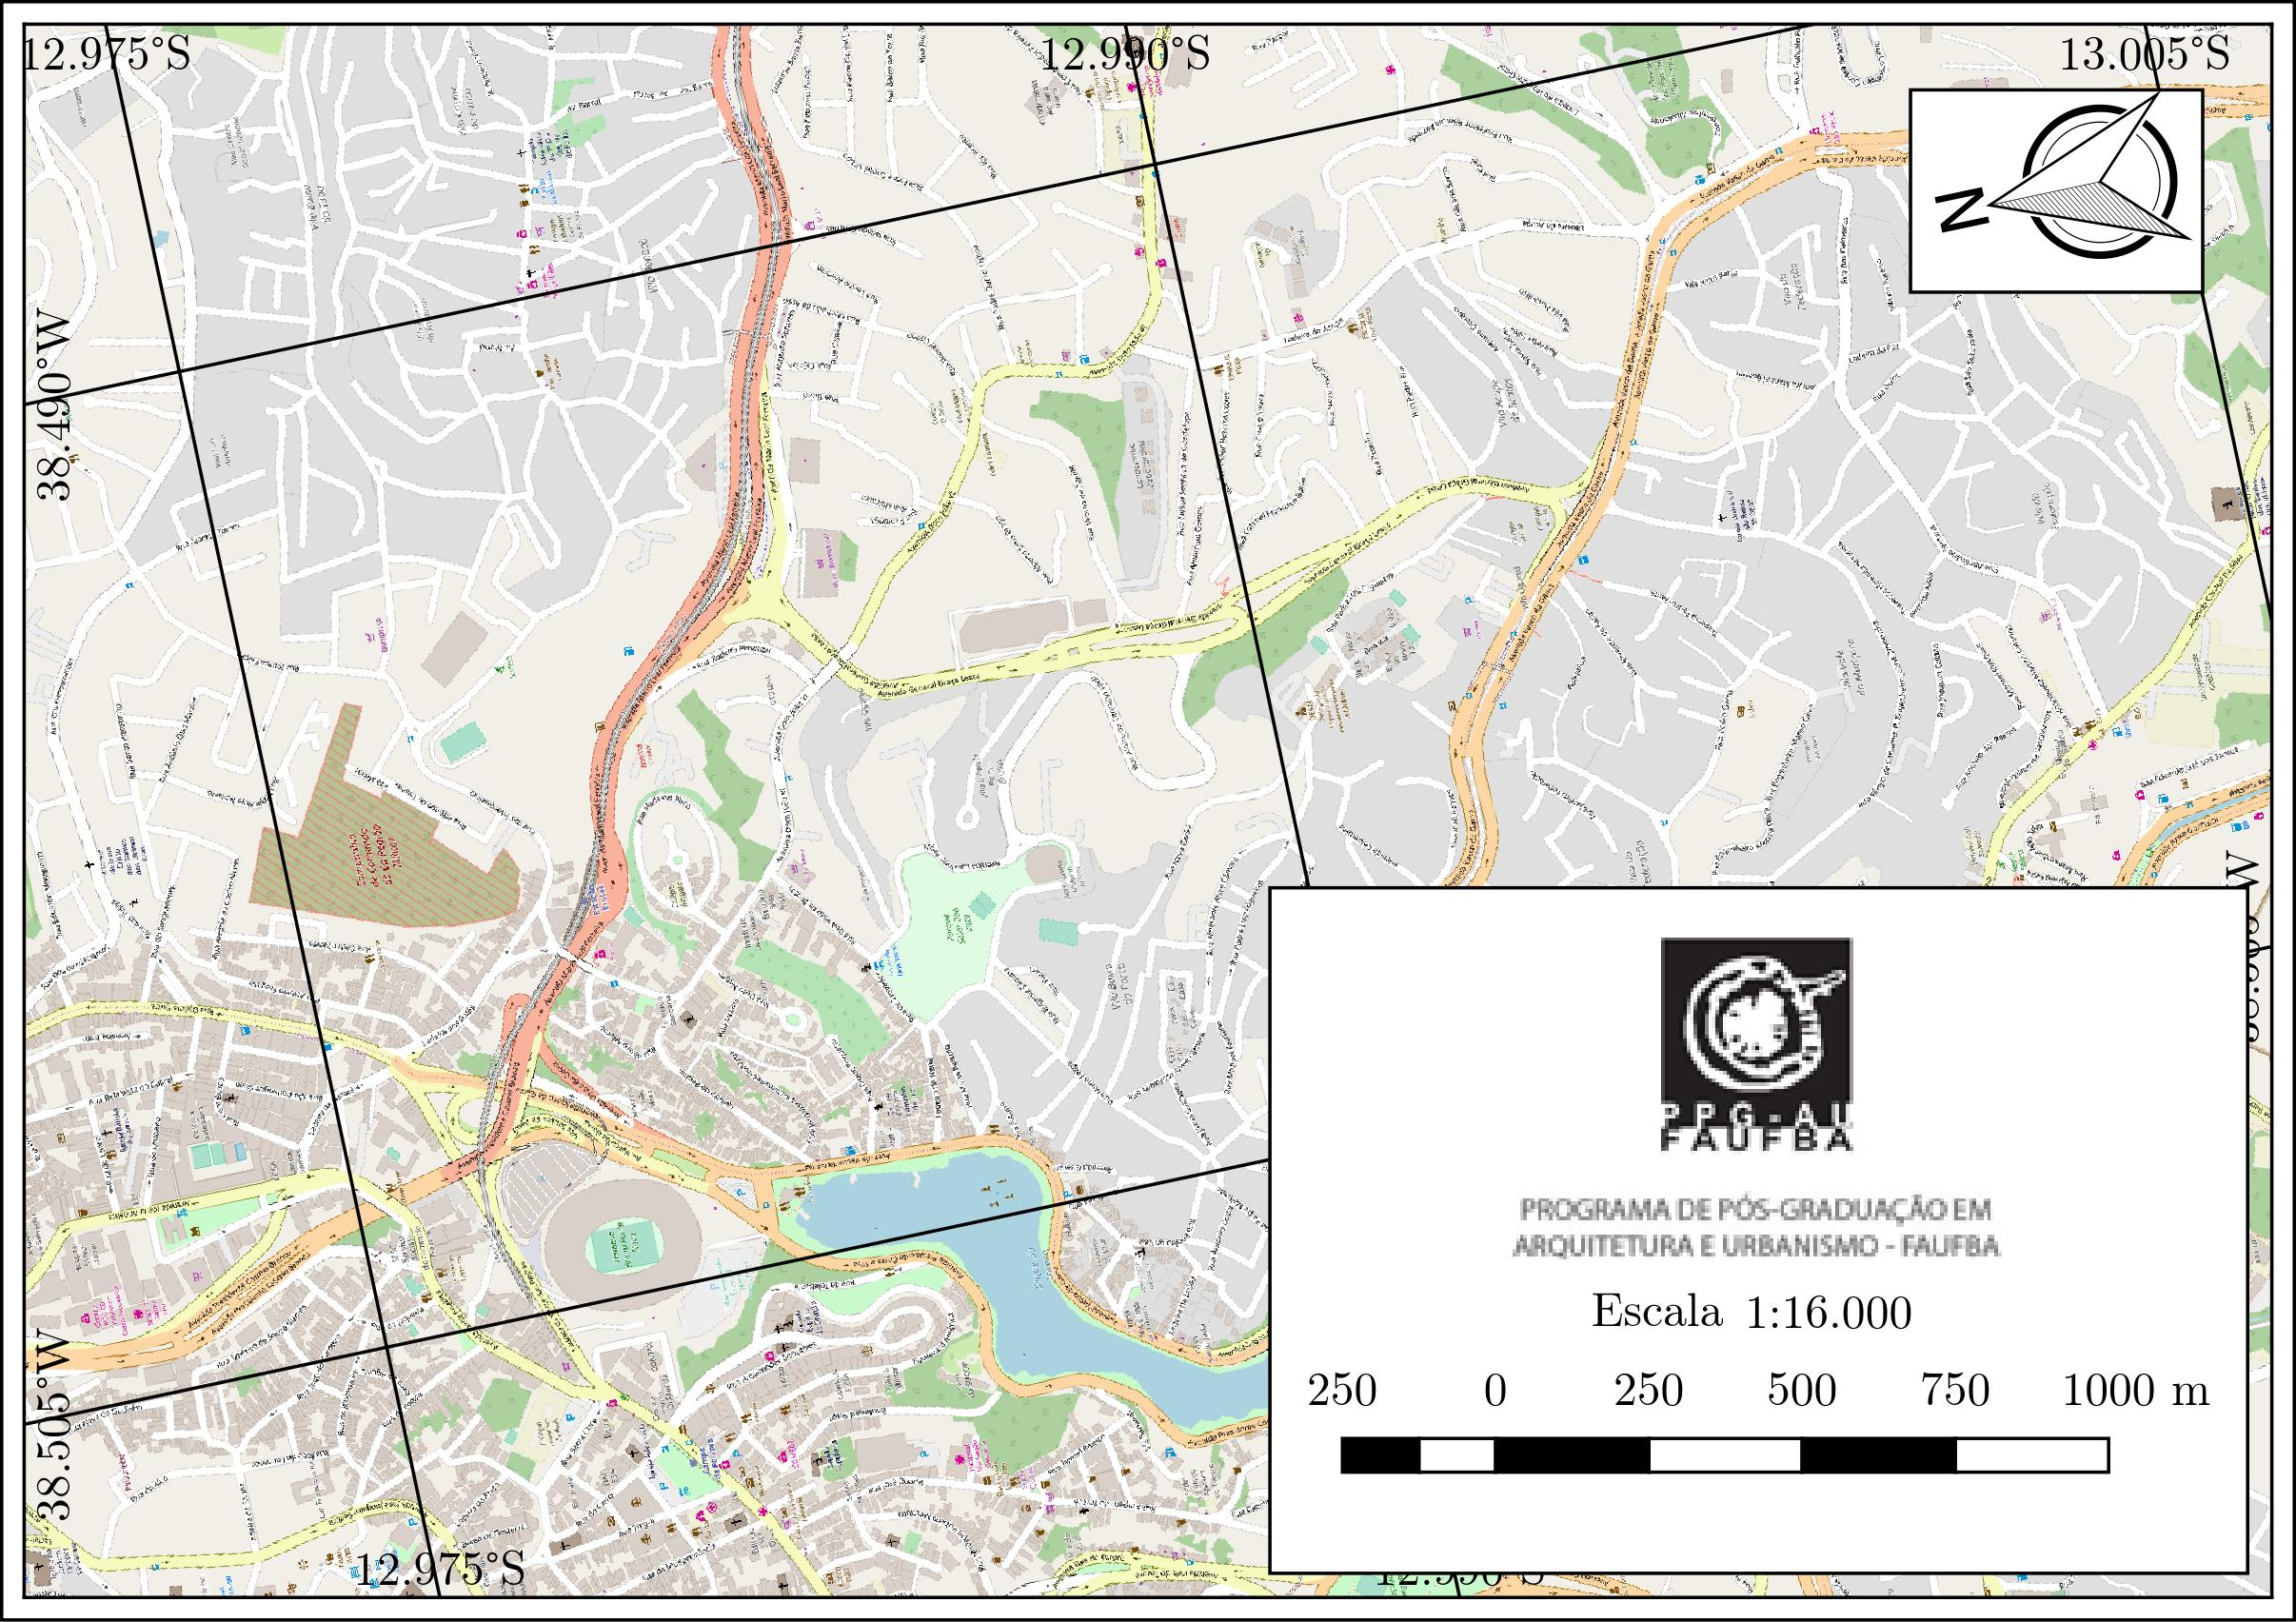
\includegraphics[width=0.8\textwidth]{3-cap2/complementos/mapas/georreferenciamento/boavista/boavista-sangradouro-2016.eps}{\footnotesize \par \textbf{Fonte:} Elaboração do autor com imagem do Open Street Maps. Respeitou-se o traçado de \citeonline{weyll_mappa_1851}. \par}
\caption{Representação cartográfica parcial da área entre a rua do Sangradouro e a avenida Cardeal da Silva}
\label{fig:boavista2016}
\end{sidewaysfigure}

O mapa de \citeonline{weyll_mappa_1851} mostra ainda uma longa estrada saindo das terras da Boa Vista em direção a uma estrada que corresponde à atual avenida Cardeal da Silva. Remanescentes desta estrada são as ruas Almirante Alves Câmara e Padre Luiz Figueira, no Engenho Velho de Brotas, e Sérgio de Carvalho, no Vale da Muriçoca; mais ou menos no ponto onde a rua Sérgio de Carvalho faz esquina com a atual av. Edite, também no Vale da Muriçoca, o mapa de Weyll indica uma ponte sobre um riacho, e daí em diante a estrada seguia um curso hoje inexistente, que terminava aproximadamente na altura da atual Ladeira das Carmelitas, na Federação. 

Em 1872 funcionava na rua da Boa Vista a taverna de Maria Amelia de Lima \cite[terceira~parte, pp.~48]{pimenta_almanak_1872}, e o ``moinho do Dique'' era mencionado num relatório provincial de 1874 \cite[p.~26]{bahia_rpe_1874b}.

O \textbf{Atlas parcial da cidade do Salvador}, mandado publicar pela Prefeitura de Salvador em 1955, apresenta uma configuração toponímica e física do Engenho Velho de Brotas muito próxima daquela encontrada durante a Primeira República\footnote{Só foi possível utilizar o \textbf{Atlas parcial da cidade do Salvador} a contento na medida em que suas informações foram cotejadas com a documentação pesquisada e com o mapa de \citeonline{weyll_mappa_1851} (cf. \autoref{fig:atlasenvgelho1955}); trata-se de documento produzido muito posteriormente ao período estudado, quando já se haviam verificado grandes modificações no tecido urbano de Brotas por força da intensificação da urbanização ocorrida no distrito durante a era Vargas (1930-1945). No que diz respeito a toponímicos e a localizações aproximadas de pontos notáveis, entretanto, trata-se de fonte documental preciosíssima, desde que, ressalte-se ainda outra vez, cotejado com outras fontes e documentos para estabelecer o que dele se aproveita e o que dele é posterior ao período pesquisado.}; nele, interessam particularmente os seguintes aspectos:

\begin{sidewaysfigure}[!htp]
% entering
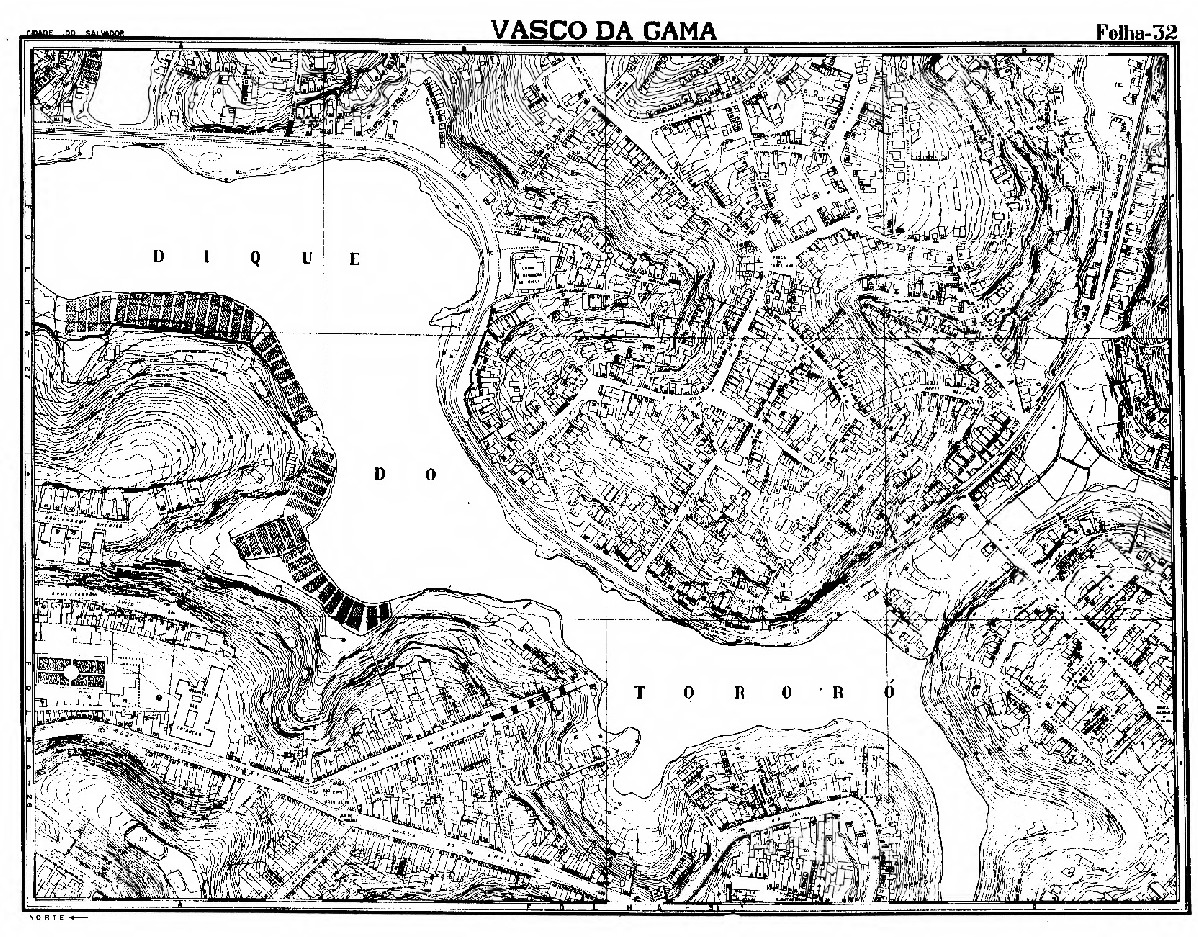
\includegraphics[width=0.8\textwidth]{3-cap2/complementos/mapas/apcs1955-f32-engvbro.eps}{\footnotesize \par \textbf{Fonte:} \citeonline{municipal_atlas_1955}. O Engenho Velho de Brotas é a área acima do Dique do Tororó. \par}
\caption{Folha 32 do \textbf{Atlas parcial da cidade do Salvador}.}
\label{fig:atlasenvgelho1955}
\end{sidewaysfigure}

\begin{enumerate}
\item A atual rua Brígida do Vale corresponde à região circunvizinha à \textit{Capela do Deus Menino}, que, a julgar pela documentação consultada e por duas obras de referência pesquisadas \cite{municipal_atlas_1955,souza_guia_1935}, teve vários toponímicos ao longo do tempo (\textit{Rua da Capelinha}, \textit{Alto da Capelinha} etc.).
\item A rua denominada na documentação encontrada como Monte de Belém é na verdade o topônimo de uma pequena área subdividida em três em três: \textit{Monte Belém de Cima}, \textit{Monte Belém de Baixo} e \textit{Monte Belém do Meio}. Estas ruas, que mantiveram seus nomes até hoje, situam-se na encosta adjacente à atual rua Brígida do Vale.
\item A \textit{Vila América} e o \textit{Alto do Moinho}, encontrados na documentação pesquisada, são duas pequenas localidades vizinhas situadas numa encosta que dá de frente para a atual avenida Vasco da Gama.
\item A julgar pela comparação entre o \textbf{Atlas} e a documentação pesquisada, a atual \textit{ladeira da União} (também conhecida como \textit{Estrada da União}) já era conhecida por este topônimo desde pelo menos o final do século XIX, e era adjacente ao \textit{porto dos Saveiros}, no Dique do Tororó.
\item Próximo ao canto superior esquerdo do mapa pode-se ver o \textit{Dique Pequeno}, constante na documentação pesquisada e hoje aterrado, correspondente à área onde hoje se situam a rua Jornalista Archimedes Gonzaga e a rua Dique Pequeno.
\end{enumerate}

\subsection{A Estrada de Brotas e seus arredores}\label{subsec:estrabrotas}

\begin{figure}[!htp]
\centering
\subfloat[Em 1851. \textbf{Fonte:} elaboração do autor, com base em \citeonline{weyll_mappa_1851}.]{
\includegraphics[width=0.4\textwidth]{3-cap2/complementos/mapas/estbrotas-1851.eps} 
\label{fig:estbrotas-1851}
 }
\  %espaco separador
\subfloat[Atualmente. \textbf{Fonte:} elaboração do autor, com base em imagem do Google Earth.]{
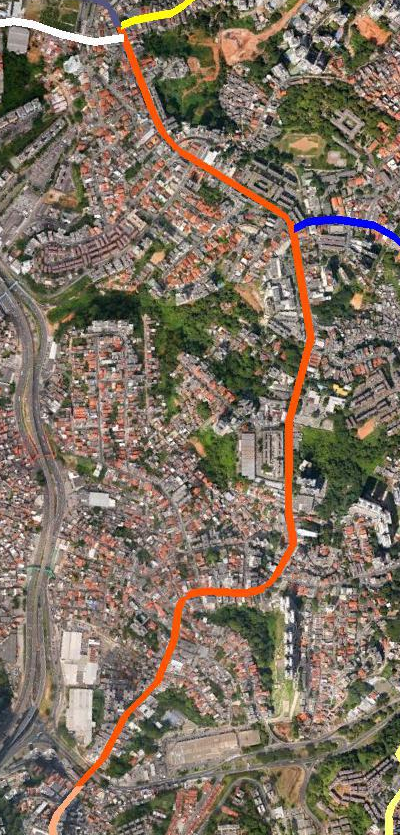
\includegraphics[width=0.4\textwidth]{3-cap2/complementos/mapas/estbrotas-hoje.eps} 
\label{fig:estbrotas-hoje}
 }
\caption{Duas representações cartográficas do território correspondente à Estrada de Brotas (atual av. D. João VI).}
\end{figure}

O segundo distrito de Brotas, ao contrário do que se sucedia no primeiro, passava por transformações muito lentas. Apesar da chegada de alguns serviços públicos infraestruturantes e da riqueza de algumas casas, o caráter rural deste distrito da freguesia permaneceu bastante marcado por todo o século XIX. Para entender o processo de urbanização e sua velocidade será necessário analisar o segundo distrito da freguesia localidade por localidade, tal como feito no primeiro distrito.

No século XVIII saía do Portão da Piedade uma estrada então conhecida como \textit{Caminho Grande}, correspondente ao que veio depois ser a \textit{Estrada de Brotas}, atual Avenida D. João VI; era por aí que se partia da cidade ao Rio Vermelho, passando pelo paço do Acupe, hoje inexistente, integrante do morgado da Casa da Torre \cite[p.~85]{campos_brotas_1942}. Patente de sargento-mor da freguesia de ``Nossa Senhora de Brotas do Caminho Grande'' concedida a Veríssimo de Campos de Carvalho em 1725 \cite[p.~114]{texmel_manusbn_1896} mostra como era conhecida a freguesia em seus primórdios.

Infelizmente não foi possível encontrar registros seguros do traçado completo do Caminho Grande, exceto por uma referência que o qualificou como `perigoso'' e disse passar ele ``pela Lapa e atual Campo da Pólvora, pela crista dos montes e pelos divisores de águas, passando em Fonte Nova e por Brotas até aquele ponto da costa oceânica'' \cite[p.~488]{sampaio_salvador_2016}. Com base no mapa de \citeonline{weyll_mappa_1851} (cf. \autoref{fig:estbrotas-1851}), pode-se conjecturar, entretanto, que a ligação entre a Piedade e o atual Largo do Paranhos, onde tinha início a Estrada de Brotas, fosse feita pelo trecho da atual avenida Joana Angélica que vai até a ladeira da Fonte Nova e por esta própria ladeira, chegando, através da atual ladeira dos Galés, até o referido largo, completando assim o primeiro trecho. Daí em diante, pode-se apenas conjecturar, inconclusivamente, por onde o Caminho Grande desceria rumo ao Rio Vermelho.

O jornal quinzenal \textbf{A Lei}, num breve perfil biografico, indicou que em 1848 o brigadeiro Evaristo Ladislau e Silva ``concorreu para o melhoramento da estrada de Brotas''\footnote{\textbf{A Lei}, ano 2, nº 2, fev. 1877, pp. 2-3.}; certamente terá a ver com o fato de que entre 1848 e 1849 a presidência da província investiu 2:269\$344 na Estrada de Brotas, comprometendo-se a investir outros 5:000\$000 em melhoramentos na via; investiu também 1:414\$000 no encanamento do rio Camorogipe, empenhando-se a investir outros 177:539\$000 na mesma finalidade \cite{bahia_rpe_1849}.

Residiam na estrada de Brotas em 1872 o major Joaquim Ignacio da Camara Pinheiro, terceiro juíiz de paz da freguesia \cite[segunda~parte, p.~91]{pimenta_almanak_1872}; José Teixeira Bahia, subdelegado de polícia de Brotas \cite[segunda~parte, pp.~132]{pimenta_almanak_1872}. Funcionavam em 1872 na estrada de Brotas as tavernas de Aprigio Monteiro Carvalho, Francisco José Gomes e José Bernardino de Almeida \cite[terceira~parte, pp.~39, 42, 43]{pimenta_almanak_1872}; o consultório do médico Francisco Xavier dos Reis, o escritório do despachante de polícia Moysés Monteiro Pereira, o ponto de aluguel de carroças de Manoel Francisco da Costa e a tipografia de Pedro Vasques de Moura \cite[quarta~parte, pp.~4, 10, 20, 38]{pimenta_almanak_1872}.

Como a Estrada de Brotas era -- e continua sendo, se somarmos as atuais ruas que estão sobre seu antigo leito -- muito comprida, é preciso fazer como os da época e subdividi-la em alguns pontos notáveis e cercanias.

\subsubsection{Largo de Brotas e Cruz da Redenção}\label{subsubsec:brotasredencao}

O primeiro ponto notável a ser analisado é o \textit{largo de Brotas}, existente desde a fundação da igreja matriz. Próximos dele existem o largo e a ladeira da \textit{Cruz da Redenção}. As duas áreas são contíguas; quem hoje sobe a ladeira da Cruz da Redenção e vira à esquerda ainda hoje sai na frente da igreja de Brotas, onde se localizava o largo de Brotas, hoje soterrado pela expansão imobiliária.

Apesar de um célebre memorialista afirmar que o largo da Cruz da Redenção foi mandado abrir em 1841 na Estrada de Brotas pelo coronel João Ladislau de Figueredo e Mello, dono do engenho Campinas \cite[p.~88]{campos_brotas_1942}, já se encontra anúncios de venda de roça na mesma localidade em 1838\footnote{\textbf{Correio Mercantil}, vol. 3, nº 583, 19 out. 1838, p. 4.}. Caetano Vicente de Almeida Galião, juiz de paz do segundo distrito da Sé em 1835, possuía um pequeno engenho e uma pequena fazenda na localidade \cite[p.~239]{REIS2004males}.

O \textbf{Livro Eclesial de Registro de Terras da Freguesia de Brotas} menciona a existência na localidade de propriedade do sr. José Joaquim de Santa Tereza, magnate local e candomblecista mestiço cujo patrimônio foi devassado na \autoref{subsec:pitangueiras} (p. \pageref{subsec:pitangueiras}). Rosa Ladislau de Figueiredo e Mello\footnote{Equivocadamente nomeada pelo \textbf{BR BAAPB} como ``Ladislau de Figueiredo Melo'' em seus registros eletrônicos.} era outra pessoa de riqueza e gosto a ter terras registradas em seu nome na localidade; como seu patrimônio será tratado com mais extensão e centralidade na \autoref{subsec:campinasladislau} (p. \pageref{subsec:campinasladislau}), vale apenas registrar sua presença nesta localidade\footnote{Trata-se muito provavelmente da casa que fora legada a Rosa por seu pai, João Ladislau de Figueredo e Melo, de cujo inventário se falará adiante.}. O \textbf{Livro} menciona ainda terreno registrado em nome de Antonio Pereira do Rio:

\begin{citacao}
Roça de Antonio Pereira do Rio

Ilustríssimo senhor Antonio Pereira do Rio possue duas roças unidas na Cruz da Redempção, freguesia das Brotas, com as divisorias seguintes. Principiando na estrada junto à casa que serve de estrebaria por hum caminho que leva para huma das referidas roças por entre duas carreiras de árvores pela parte do nascente a dividia com outra roça pertencente a José Esteves Barretto, e chegando a huma taipa de frente esta ao meio a [ilegível] huma valla que divide a mesma roça por vertentes até mais abaixo encontrando com outra roça do vigário Antonio Segundo da Rocha até o rio Camorogipe e por este abaixo divisando-se com terras dos herdeiros do Visconde do Rio Vermelho até outra valla que corre para o mesmo rio e por ela acima divisa-se com J[ilegível] Maria de Jesus até huma cerca que sobe em hum pé de jaqueira na estrada da Ubarana e subindo pela estrada até o largo da Cruz da Redempção. Antonio Pereira do Rio. E nada mais continhão as declarações que me foram enviadas. Brotas da Bª, 17 de julho de 1858. Vigº Ernesto de Oliveira Valle\footnote{\textbf{BR BAAPB}, fundo Colonial, série Registros de Terra, livro 4675, f. 33 verso.}
\end{citacao}

Daqui se pode extrair a informação de que a atual ladeira da Cruz da Redenção era conhecida em meados do século XIX como \textit{estrada da Ubarana}.

Residiam no largo de Brotas em 1872 o pároco Ernesto de Oliveira Valle; Francisco Ovídio de Aguiar Pantoja, arborizador da Inspetoria de Obras da Câmara Muncipal; Mathias de Jesus Nogueira, escrivão do juízo de paz da freguesia; e João Américo Gomes, escrivão da subdelegacia de polícia de Brotas; \cite[segunda~parte, pp.~69, 87, 91, 132]{pimenta_almanak_1872}. Funcionavam em 1872 no largo de Brotas as taverna de Caetano Gomes da Costa Farias e Tibério José do Espírito Santo \cite[terceira~parte, pp.~40, 49]{pimenta_almanak_1872}, e o escritório do agente de causas Evaristo José de Santa Anna Gomes \cite[quarta~parte, pp.~6, 8]{pimenta_almanak_1872}.

Nada há qualquer registro sobre a Cruz da Redenção nos almanaques consultados, indício da baixa presença na localidade de serviços urbanos, de residências de funcionários públicos ou de escritórios, consultórios e oficinas. Em 1882 uma casa posta a leilão nesta localidade foi assim descrita e avaliada:

\begin{citacao}
Uma casa situada à rua da Redempção, freguezia de Brotas, com 3 metros e 30 centimetros de frente, e n'esta uma porta e janella, sala, dous quartos, sala de jantar em commum com a cosinha, pequeno quintal; divide-se por um lado com casa do intestado e pelo outro com Luiz Mendes, avaliada por 100\$000\footnote{\textbf{Diário da Bahia}, 3 jan. 1889, p. 2.}.
\end{citacao}

Em 3 de março de 1889 petição de moradores de Brotas ao chefe de polícia implorava providências contra ``aos abusos, ás desordens, aos sambas, ás palavras, gestos immoraes, e a toda sorte de escandalos que se praticão n'este infeliz logar, de onde a policia parece ter fugido espavorida''; reclamam da ``constante mutação de physionomias que, á semelhança de morcegos, apparecem e desapparecem quotidianamente'', e pedem ``amplas e energicas medidas que os garantam da sanha dos desordeiros, para que continuem a viver tranquilos como até aqui têm vivido n'esta agreste solidão''\footnote{\textbf{Diário da Bahia}, nº 50, 3 mar. 1889, p. 2.}. Ditos ``moradores ordeiros'' voltariam à carga ainda outra vez em 14 de março para falar de um ``crioulo conhecido em toda a freguezia de Brotas, principalmente do largo da matriz até á Cruz da Redempção, como perigoso desordeiro'' que teria sido responsável pelo assassinato do fiscal João Cancio Vergne Baptista e era ``capaz de commeter crime de qualquer natureza que lhe seja ordenado''; esta mesma pessoa teria causado desordem na festa da Pituba, ocorrida no mês anterior, ``pondo em sobresalto aos moradores da povoação''. Apontando diversas vezes relações de proximidade entre as autoridades policiais e a pessoa em questão, suplicavam ao presidente da província para que fizesse sentir ao chefe de polícia que ``o povo do largo da Matriz e da Cruz da Redempção, em Brotas, tem direito tambem a ser mantido pela força publica'' ; como o subdelegado da freguesia, diversas vezes procurado sobre a questão, ``limita-se a dizer que não dispõe de força publica'', chegaram mesmo a oferecer casa para que o destacamento de polícia da freguesia fosse dividido, ficando metade dele no largo de Brotas ou na Cruz da Redenção\footnote{\textbf{Diário da Bahia}, 14 mar. 1889, p. 2.}.

\subsubsection{Cemitério de Brotas}\label{subsubsec:cemitbro}

No que diz respeito ao \textit{cemitério de Brotas}, construído sobre terras anteriormente pertencentes ao desembargador Manoel Maria do Amaral \cite[relatório da inspetoria de higiene, p.~23]{bahia_rpe_1893}, é preciso antes de mais nada desfazer um equívoco historiográfico. Relato de Francisco Vicente Vianna \cite[p.~371]{vianna_bahia_1893} induziu a erro tanto \citeonline{VASCONCELOS2002} quanto \citeonline{flexor_desenho_1999}; segundo este relato, a necrópole teria sido fundada em 1876, mas viu-se na documentação pesquisada que já em 1869 havia inumações no local\footnote{\textbf{Gazeta Medica da Bahia}, vol III, 1869, p. 95}, que em 1871 este cemitério já demandava ser alargado\footnote{\textbf{Jornal da Bahia}, ano XIX, nº 5.446, 22 set. 1871, p. 1} e que em 1872, quando estava sob administração do vigário Ernesto Oliveira Valle \cite[segunda~parte, p.~105]{pimenta_almanak_1872}, ele deixara de funcionar por quatro meses e já não satisfazia as necessidades funerárias dos moradores da freguesia, pelo que se propunha então construir outro cemitério no Acupe \cite[relatório do chefe de polícia, p.~12]{bahia_1872}. Em 1873 foi nomeado como administrador deste cemitério Quod Vult Deus da Silva Valle \cite[p.~39]{bahia_rpe_1873a}, demitido alguns anos depois a bem da administração pública. Entre 1874 foi autorizada a construção de uma cerca no entorno da necrópole, que no ano seguinte ainda não havia sido concluída por ``falta no mercado de estacas d'aderno, de 1ª qualidade'' \cite{bahia_rpe_1874,bahia_rpe_1875}.

Deduz-se de tudo isto que sua fundação ocorreu em data anterior\footnote{\citeauthoronline{flexor_desenho_1999}, com base na Lei do Orçamento Provincial nº 1.131, indica que ``desde 1870 o governo autorizara a compra de um terreno na freguesia de Brotas, em frente da Cruz da Redenção, para estabelecer um cemitério público'', mas diz, imediatamente em seguida, que ``a reação contra os enterramentos, fora ou longe das igrejas, retardou a iniciativa'' (\citeyear{flexor_desenho_1999}, p. 104), deixando a data de fundação do cemitério como 1876.}, mas nem a documentação pesquisada nem a bibliografia consultada permitiram precisá-la em definitivo. O que de fato ocorreu em 1876 naquele cemitério foram, na verdade, o anúncio de sua ``inauguração'' em dezembro de 1875 \cite[p.~54]{bahia_rpe_1876}, que tem mais jeito de \textit{reinauguração} em seguida a \textit{reformas} demarcadoras de sua encampação pela administração pública; e o requerimento, no dia 4 de julho, por parte do juiz e mesário da irmandade do Santíssimo Sacramento de Nossa Senhora de Brotas, de 30 metros quadrados de terreno devoluto para a construção de carneiros para a irmandade\footnote{\textbf{O Monitor}, 16 jul. 1876, p. 2}. 

Em 1879 a presidência da província transferiu a administração do cemitério para a Câmara Municipal por meio da lei 1.943, de 26 de agosto do mesmo ano\footnote{\textbf{O Monitor}, 30 ago. 1879, p. 1.}. Relatórios anuais dos presidentes da província da Bahia de 1876 em diante indicam estar esta necrópole, a única pública em meio a cemitérios administrados por irmandades religiosas, sempre em bom estado de conservação e asseio. Não foram encontrados na documentação pesquisada quaisquer outras referências além de atos burocráticos e estatísticas mortuárias; dado o caráter mórbido deste imóvel, é de se esperar que poucos se interessassem por sua vizinhança.

\subsubsection{Estrada e Alto do Beiju}\label{subsubsec:estrbeiju}

A localidade conhecida no século XIX e começo do século XX como \textit{Alto do Beiju}, limite extremo da Estrada de Brotas onde tinha origem a \textit{Estrada do Beiju} ou \textit{Estrada das Armações}, situava-se nas cercanias do cemitério de Brotas. Vista a partir do mapa de \citeonline{weyll_mappa_1851}, a estrada é o caminho que tem início no cemitério de Brotas e segue até sumir do mapa; sobreposto o mapa de Weyll a um mapa atual, tudo indica tratar-se da atual rua Teixeira Barros, que de algum modo ligava-se com a atual avenida Paulo VI lá onde o mapa de Weyll termina. Se esta sobreposição corresponder ao que realmente existiu, pode-se dizer que a rua Teixeira Barros e a avenida Paulo VI são plurisseculares, e que compunham um só caminho a ligar Brotas com as armações do Saraiva e do Gregório, na orla atlântica de Salvador.

O \textbf{Livro Eclesial de Registro de Terras da Freguesia de Brotas} menciona a existência de terrenos registrados em nome do tenente Bernardino José de Almeida, assim descritos:

\begin{citacao}
Roça de Bernardino José de Almeida

Bernardino José de Almeida é possuidor da roça sita à Ladeira do Beijú, freguesia de Nossa Senhora das Brotas, a qual limita-se de um lado com a roça de hum Olegario Vieira e do outro lado com o rio Camorogipe e o fundo com a roça de Antonio Pereira do Rio. Bernardino José de Almeida. E nada mais continhão as declarações que me forão apresentadas. Brotas da Bª, 13 de julho de 1858. Vigário Ernesto de Oliveira Valle\footnote{\textbf{BR BAAPB}, fundo Colonial, série Registros de Terra, livro 4675, f. 26 frente.}
\end{citacao}

Este mesmo Bernardino José de Almeida morreu em 1876 numa roça em Brotas e, por falta de meios, ficou tres dias insepulto, inumado por ato de benemerencia de ``certo escrivão Gularte''\footnote{\textbf{O Alabama}, ano 14, serie 163, nº 1625, 25 nov. 1876.}, também ele residente à estrada do Beiju, como fez questão de registrar em letras garrafais num protesto contra erro em seu alistamento eleitoral:

\begin{citacao}
\textbf{Á Junta parochial de Brotas ou a cada um de seus membros}

No \textit{Diario da Bahia} apparece na \textit{confusa} lista publicada hoje, o meu nome com a nota -- \textit{mudado}.
Nada importa esta declaração feita, por aquelles que ignoram a lei, além de não ter valor algum semelhante alistamento, visto não ter sido annullado o anterior, de cuja junta fui um de seus membros; mas para que não fique sem protesto de minha parte semelhante \textit{covardia}, provoco-os a vir á imprensa indicar o meu domicilio fóra da roça á estrada das armações, logar denominado Beijú, d'essa freguesia.
Si presam a dignidade venham apontar minha morada ainda mesmo sem documentos.
Bahia, 24 de abril de 1879.
\textsc{Joaquim Gularte da Silva}\footnote{\textbf{Gazeta da Bahia}, ano I, nº 92, 25 abr. 1879, p. 2}
\end{citacao}

Outra moradora da Ladeira do Beijú era Thomasia Bemvinda de Aquino, cuja posse foi assim registrada:

\begin{citacao}
Roça de Thomasia Bemvinda de Aquino

Thomasia Bemvinda de Aquino possue um terreno sito na ladeira do Beijú, Freguesia de Nossa Senhora das Brotas desta Capital, [ilegível] por um lado e pelo fundo com terras dos herdeiros do finado coronel João Ladislau de Figueiredo e Mello, por outro com Francisco Antonio [ilegível] e na frente pela estrada que vai para as Armações. Freguesia de Brotas, trinta e um de maio de mil oitocentos e cinquenta e oito. Thomasia Bemvinda de Aquino. E nada mais continhão as declarações que me foram enviadas. Brotas da Bahia, 2 de junho de 1858. Vigº Ernesto de Oliveira Valle\footnote{\textbf{BR BAAPB}, fundo Colonial, série Registros de Terra, livro 4675, f. 4 verso.}. 
\end{citacao}

Nada mais foi possível encontrar na documentação pesquisada e na bibliografia consultada acerca desta área, demonstrando ou sua baixa povoação, ou sua povoação por gente condenada a uma pobreza tão extrema e miserável que sequer deixou rastro em documentos públicos ou na imprensa.

\subsubsection{Cruz das Almas}\label{subsubsec:cruzalm}

\textit{Cruz das Almas}, reiteradamente encontrada na documentação pesquisada, foi localidade difícil de situar. O \textbf{Livro Eclesial de Registro de Terras da Freguesia de Brotas} registra a existência, na Cruz das Almas, de uma propriedade de Herculano Nunes dos Reis:

\begin{citacao}
Roça do Tenente Herculano Nunes dos Reis

Segunda rua da Cruz das Almas para o Rio Vermelho -- Freguesia de Brotas -- Proprietário Herculano Nunes dos Reis, tendo de frente noventa braças dividida com José Teixeira Bahia e Florêncio Benjamin de Almeida Pires e pelo fundo com Antonio José Ferreira e doutor Salustiano José Pedrosa, havendo adquirido a mesma propriedade por herança de meus pais Cipriano Nunes dos Reis e dona Rita Maria de Assumpção Reis e [ilegível] de terras [ilegível] [ilegível] herdeiros. Bahia, oito de julho de mil oitocentos e cinquenta e sete. Herculano Nunes dos Reis. E nada mais continhão as declarações que me forão enviadas. Brotas da Bahia, 2 de setembro de 1857. Vig.º Ernesto de Oliveira Valle\footnote{\textbf{BR BAAPB}, fundo Colonial, série Registros de Terra, livro 4675, f. 02 frente.}.
\end{citacao}

Registra também o \textbf{Livro} na localidade uma posse de Francisca de Sales Bahia:

\begin{citacao}
Roça de D. Francisca de Sales Bahia

Dona Francisca de Sales Bahia é possuidora usufructuaria da roça à Cruz das Almas desta freguesia a qual tendo duas frentes, uma na estrada de Brotas com a extensão de trinta e uma braças, outra na do Rio Vermelho com a de duzentos e setenta, limita-se pela frente com roça de José Francisco de Bellas, partindo da estrada em linha [ilegível] até o brejo e dahi em diante, digo e dahi em linha recta por uma valla onde também divide-se com a roça chamada Engenhoca até encontrar a de Luiz Antonio Ferreira, donde partindo em linha recta ou quasi com cerca nativa, e dahi divide com a de Herculano Nunes dos Reis vai terminar-se com a estrada do Rio Vermelho. Bahia e Freguesia de Nossa Senhora das Brotas, quatorze de julho de mil oitocentos e cincoenta e oito. Por minha mãe a Senhora Dona Francisca de Sales Bahia, José [ilegível] Bahia. E nada mais continhão as declarações que me forão enviadas. Brotas da Bª, 14 de julho de 1858. Vigº. Ernesto de Oliveira Valle\footnote{\textbf{BR BAAPB}, fundo Colonial, série Registros de Terra, livro 4675, f. 27 frente.}.
\end{citacao}

Daqui se deduz que \textit{Cruz das Almas} era a localidade, e a \textit{estrada da Cruz das Almas}, tantas vezes referida na documentação pesquisada, pode ter sido outro nome para o que se encontra seis vezes no \textbf{Livro Eclesial de Registro de Terras da Freguesia de Brotas} como \textit{estrada de Brotas para o Rio Vermelho}. Se esta hipótese for verdadeira, a \textit{Cruz das Almas} seria a localidade situada no cruzamento entre as atuais avenidas Waldemar Falcão e D. João VI, e a estrada da Cruz das Almas, ou estrada de Brotas para o Rio Vermelho, seria a atual avenida Waldemar Falcão. Parece ter sido esta a situação, a julgar pelos outros seis registros.

Já em 1870, um certo Miguel dos Santos Prates vinha a público agradecer aos que acompanharam o cortejo fúnebre de seu pai desde sua casa, na estrada da Cruz das Almas, até o cemitério de Brotas\footnote{\textbf{O Monitor}, 20 jun. 1870, p. 3}. Residiam na Cruz das Almas em 1872 José Marcellino Moreira Sampaio, engenheiro, segundo juiz de paz da freguesia e professor de francês do Liceu da Palma \cite[segunda~parte, pp.~96]{pimenta_almanak_1872}; nada mais foi possível encontrar acerca da localidade na documentação pesquisada e na bibliografia consultada.

Dois africanos que moravam no caminho de Brotas para o Rio Vermelho foram encontrados mortos, e a policia prendeu um crioulo de mais de 60 anos como suspeito do latrocínio \footnote{\textbf{Jornal da Bahia}, ano XXII, número ilegível, 10 mar. 1875, p. 2}; importa aqui menos a ocorrência que o fato de ela evidenciar a moradia de \textit{africanos} e \textit{crioulos} na área.

\subsection{A Estrada Dois de Julho: elefante branco ou ermo dos pobres?}\label{subsec:e2j}

\begin{figure}[!htp]
\centering
\subfloat[Em 1851. \textbf{Fonte:} elaboração do autor, com base em \citeonline{weyll_mappa_1851}.]{
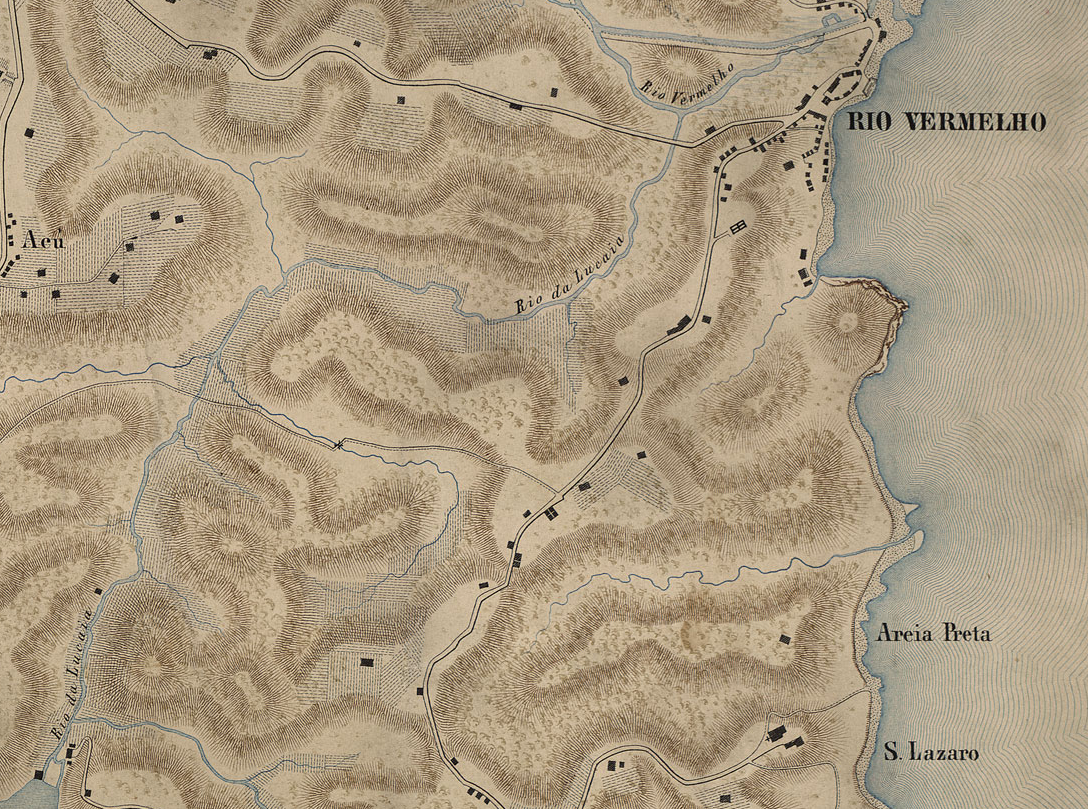
\includegraphics[width=0.7\textwidth]{3-cap2/complementos/mapas/e2j-1851.eps} 
\label{fig:e2j-1851}
 }
\  %espaco separador
\subfloat[Atualmente. \textbf{Fonte:} elaboração do autor, com base em imagem do Google Earth.]{
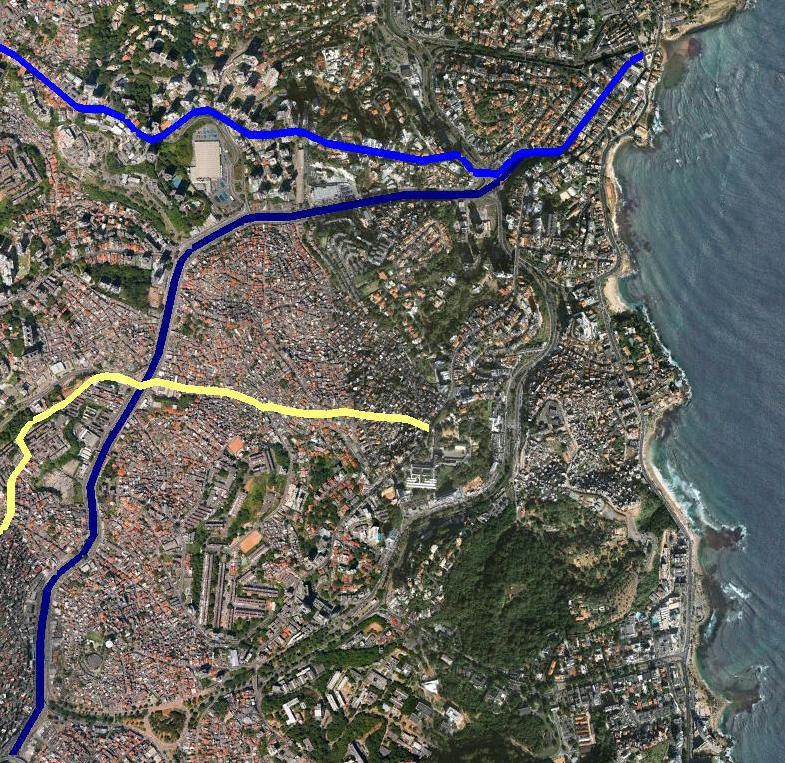
\includegraphics[width=0.7\textwidth]{3-cap2/complementos/mapas/e2j-hoje.eps} 
\label{fig:e2j-hoje}
 }
\caption{Duas representações cartográficas da Estrada Dois de Julho (atual av. Vasco da Gama).}
\end{figure}

A \textit{estrada Dois de Julho}, hoje conhecida pelo menos desde 1935 como \textit{avenida Vasco da Gama} \cite[p.~142]{souza_guia_1935}, foi inaugurada em 1859 como caminho alternativo entre o arrabalde do Rio Vermelho e a zona urbana de Salvador; seu trajeto corre rente ao rio Lucaia, desde sua nascente no Dique do Tororó até as vizinhanças da sua foz, no Rio Vermelho \cite[p.~582]{ruy_politica_1949}.

Já se esperava encontrar pouquíssima coisa sobre a estrada na bibliografia pesquisada, mas o que se encontrou na documentação pesquisada sobre ela foi simplesmente surpreendente: obras, obras e mais obras. A estrada Dois de Julho atravessou a segunda metade do século XIX como um verdadeiro sorvedouro de recursos públicos.

Já em 1863, quatro anos após sua inauguração, foram construídos 11 pontilhões sobre a estrada, arrematados por 5:276\$000 \cite[p.~66]{bahia_rpe_1863b}. Em 1866 foi realizada limpeza geral do mato que cobria a estrada, além do aterro de lugares alagadiços e de outros apertados e íngremes; do serviço, que gastara até o momento da preparação do relatório provincial cerca de 700\$000, se disse que ``não tem ficado barato'', mas o encarregado da obra, José Carlos Ferreira, atribuiu o alto valor investido à ``penúria de bons trabalhadores'' \cite[p.~76]{bahia_rpe_1866}. No mesmo serviço o engenheiro Aguiar observou que a colocação de canos de captaçao do esgoto das casas circunvizinhas 

\begin{citacao}
foi tão a capricho, para não dizer má, que de futuro exigirá consideráveis modificações, por serem alguns muito acanhados para as aguas a que tem de dar esgoto, e porque sem essas modificações não se poderá dar o declive conveniente á estrada \cite[p.~76]{bahia_rpe_1866}
\end{citacao}

Em 1867 o estado da via mereceu comentários azedos por parte do presidente da província:

\begin{citacao}
ESTRADA DOUS DE JULHO

Esta estrada, que parte da Fonte Nova á povoação do Rio Vermelho, contornando o Dique, aberta com pouca largura e muitas irregularidades, nunca foi concluída. Sua abertura foi iniciada pela camara municipal, mandando posteriormente o governo melhoral-a e construir diversos pontilhões de alvenaria. 
Esta obra, alias de utilidade, porque facilita o transito por um caminho plano, d'esta cidade para a referida povoação, acha-se parada. \cite[obras publicas,~p.~9]{bahia_rpe_1867}
\end{citacao}

Seria a estrada Dois de Julho um exemplo recuado do modelo de obra pública que hoje se vê a torto e a direito -- ou seja, um misto de superfaturamento e má execução? Será certamente ilustrativo quanto ao assunto ver mais detidamente a relação da empresa \textit{Trilhos Centrais}, de Francisco Justiniano de Carvalho e dos herdeiros de Rafael Ariani, com a estrada.

A Trilhos Centrais pretendia prolongar sua linha da Fonte das Pedras ao Rio Vermelho. Acontece que Antonio de Lacerda, dono da \textit{Companhia de Transportes Urbanos} e cessionário do privilégio concedido pela lei provincial 1.231, de 12 de junho de 1872 para construir o que veio a ser posteriormente conhecido como a ``máquina do Rio Vermelho''\footnote{Tratava-se de um ``serviço de ferro-carril feito por quatro locomotivas que se revezavam duas a duas puxando três ou quatro carros'' \cite[p.~90]{trinchao_parafuso_2010}.}, disputava o setor de transportes públicos com esta empresa, e decidiu aproveitar a ocasião para atacar. Solicitou parecer à comissão de fazenda da província com base neste privilégio para remover a concorrência da Trilhos Centrais e atuar sozinho no Rio Vermelho, usando o leito da estrada Dois de Julho para instalar os trilhos de sua máquina; acontece que a Assembleia Legislativa provincial, que tinha competência legislativa para tratar do assunto, negou sua pretensão \cite[p.~250]{bahia_relatassleg_1875}, mantendo a atuação da empresa Trilhos Centrais paralela à empresa Transportes Urbanos, pois considerava-se o ramal pretendido por ela como

\begin{citacao}
\dots de summa utilidade e talvez de melhor conveniência para o público, por isso que vem entroncar-se na grande linha da Rua da Valla, sem duvida alguma a primeira arteria d'esta Capital, mormente depois que foi projectada pelos emprezarios levar até o engenho da Conceição, nas proximidades da via ferrea do S. Francisco, a construção de trilhos em prolongamento aos já por elles explorados \cite[p.~169]{bahia_rpe_1874}.
\end{citacao}

Acontece que, entre disputas, suspensões e retomadas de obra, em 31 de março de 1877 a Câmara Municipal pediu providências quanto aos aterros no Dique do Tororó promovidos durante o ``assentamento dos trilhos da linha férrea do Rio Vermelho'', pois ``as águas alli estagnadas têm causado damno à saude publica, produzindo febres intermittentes e perniciosas nos moradores das Pitangueiras, Matatú, Castro Neves e Bôa-Vista''\footnote{\textbf{Correio da Bahia}, ano VII, nº 12, 10 abr. 1877, p. 2}. As obras na ``ladeira de Joaquim José de Oliveira'' (\autoref{fig:joaquim}, p. \pageref{fig:joaquim}) devem ser vistas neste contexto, portanto. 

Em 1878 o mesmo problema permanecia em pauta, pois o presidente da província oficiou ao diretor das obras públicas para que informasse 

\begin{citacao}
qual a causa da estagnação das águas do Dique ao lado da estrada Dous de Julho, quaes os meios a empregar-se para remediar esse mal e se a empreza Trilhos Centraes é ou não obrigada pelo contracto das obras da mesma estrada a fazer os serviços necessarios para saneamento da localidade\footnote{\textbf{O Monitor}, ano II, nº 288, 18 maio 1878, p. 1.}
\end{citacao}

Ao que tudo indica a Trilhos Centrais teve de assumir a responsabilidade, pois em 10 de maio de 1879 o presidente da província ordenou ao diretor de obras públicas 

\begin{citacao}
\dots lavrar contracto n'essa repartição com o Commendador Giusto Ariani para o serviço de deseccação do terreno na estrada Dous de Julho, entre a fábrica de lapidação de diamantes pertencente aos negociantes Costa Pinto \& Filhos e a ladeira que segue para Brotas, e bem assim para a canalisação da parte do riacho Lucaia entre aquelles dous pontos\footnote{\textbf{O Monitor}, 03 jun. 1879, p. 1.}.
\end{citacao}

As obras foram feitas ao custo de 3:186\$908, e resultaram no ``dessecamento'' de dois pântanos, na construção de um cano de esgoto das águas do vale a eles contíguo e na canalização do Lucaia entre os dois pontos de referência mencionados \cite[obras~publicas,~p.~9]{bahia_rpe_1880}. Todavia, em 1880 o mesmo Ariani era acusado de ter produzido ``estragos'' na estrada; a Câmara Municipal,  ``temerosa como sempre'', parecia não se animar a cobrar-lhe os prejuízos\footnote{\textbf{A Gargalhada}, nº 4, 25 abr. 1880, p. 3}. Em 1881 a empresa Trilhos Centrais receberia ainda outros 1:223\$800 pela construção de uma ponte na estrada, pois o pontilhão sobre o rio de São Pedro existente no Moinho do dique havia sido destruído por uma cheia \cite[obras~publicas,~pp.~8,~13]{bahia_rpe_1881}.

Vista pelo prisma da relação entre a empresa Trilhos Centrais, a presidência da província da Bahia e a Câmara Municipal de Salvador, a imagem da estrada Dois de Julho como sorvedouro de recursos públicos parece reforçada. 

Mas e os moradores de suas margens? Onde estavam? Sequer a documentação pesquisada foi capaz de indicar um só que fosse no século XIX. Resta conjecturar sobre este fato e levantar hipóteses a partir das características físicas do rio Lucaia e de seu entorno. 

O rio Lucaia do século XIX era caudaloso e piscoso; sabe-se da mariscagem praticada na sua foz ainda na década de 1950 do século XX por meio de fotografias diversas. As cheias do rio, ainda perceptíveis antes de seu tamponamento em 2008, dão a entender que suas margens eram constantemente irrigadas, e portanto fertilizadas, pelas águas transbordantes. Nos dois casos, trata-se de espaços excelentes para a pesca e a agricultura, duas atividades tradicionalmente exercidas na freguesia de Brotas no século XIX (cf. \autoref{sec:2.2}, p. \pageref{sec:2.2}). A documentação pesquisada mostra que as encostas do vale formado pelo rio Lucaia, ao menos no lado pertencente à freguesia de Brotas, eram ocupadas por fazendas, roças e minifúndios; some-se a isto o fato de muitas herdades registradas no \textbf{Livro Eclesial de Registro de Terras da Freguesia de Brotas} terem o próprio Lucaia como limite e encontra-se aí o campo livre para localizar uma população rarefeita de posseiros, foreiros, rendeiros, moradores, arrendatários e escravos, invisibilizada pelos registros oficiais, mas viva e produtiva.

\subsection{Mariquita: pesca, lazer e veraneio}\label{subsec:mariq}

Apesar de o Rio Vermelho ser muito citado em toda a documentação pesquisada, em especial por se tratar de ``ponto preferencial para vilegiatura'' \cite[p.~597]{ruy_politica_1949}, sabemos que, em termos estritamente administrativos, a localidade foi separada ao meio pelo rio Lucaia, ficando com a freguesia da Vitória o lado que vai do Lucaia para a Barra e com a freguesia de Brotas o lado que vai do Lucaia para Itapuã. Corresponde este último à povoação da \textit{Mariquita}, que compreende o atual largo da Mariquita e áreas circunvizinhas. Como a etimologia e parte da história desta povoação já foram vistos na \autoref{subsec:precabral} (p. \pageref{subsec:precabral}), pode-se concentrar a atenção sem maiores prejuízos no desenvolvimento desta povoação no século XIX.

Do saneamento na Mariquita dizia-se que ``não ha anno algum em que não appareçam alli febres de máu caracter, porque as aguas em alguns logares não teem a correntesa necessaria, por accumulação de folhas podres e outros obstaculos'' \cite[p.~20]{bahia_relatassleg_1873}. Em 1877, atendendo a solicitação de moradores, a presidência da província autorizou a diretoria de obras a aterrar dois charcos existentes no Rio Vermelho, um na Mariquita e outro na Paciência\footnote{\textbf{O Monitor}, ano II, nº 74, 29 ago. 1877, p. 1}, contribuindo para melhorar a salubridade da povoação.

Em 1878 projeto de lei provincial pretendeu separar do território de Brotas uma freguesia específica para o Rio Vermelho tendo como base a capela curada existente neste então lugarejo; seus limites seriam ``os do actual districto policial'', fazendo fronteira com a freguesia da Vitória no lugar então conhecido como ``Quebrabunda'', com a freguesia de Brotas pelo rio ``Camorogipe'' e com a de Itapuã pelas ``Armações''\footnote{\textbf{O Monitor}, 23 ago. 1878, p. 1.}; embora, de fato, a Lei Provincial nº 2.016, de 20 de julho de 1880, houvesse elevado a ``capela curada de Sant'anna do Rio Vermelho'' ao \textit{status} de freguesia\footnote{\textbf{O Monitor}, 17 ago. 1880, p. 1.} com limites ligeiramente diferentes daqueles previstos no projeto de lei\footnote{``Principiará do lado da Victoria, desde a pancada do mar até o logar denominado S. Lazaro, inclusive, e seguindo em direcção à estrada real do Rio Vermelho, por esta descerá a baixa da ladeira do Quebrabunda; e depois irá em linha oblíqua até encontrar a estrada Dous de Julho e atravessando ahi o rio Lucaia, seguirá por territorio de Brotas, até atravessar a estrada real da Cruz das Almas, no limite da fazenda Misericordia, exclusive; e d'ahi descendo a encontrar o rio Camorogipe, e, atravessando este, seguirá pela margem esquerda até a ponte ou passagem que conduz à Cruz da Redempção; e d'ahi marginando sempre o mesmo rio Camorogipe, até encontrar o rio das Pedras, e por este até a pancada do mar''.}, a totalidade da documentação pesquisada demonstra, entretanto, que tal freguesia não vingou\footnote{Vários indícios apontam que esta freguesia ficou só no papel. Os sorteios de jurados para o tribunal do júri publicados em várias edições de \textbf{O Monitor} de novembro e dezembro de 1880 o Rio Vermelho já não é considerado como freguesia em separado.}, e o Rio Vermelho, já durante a Primeira República, encontrava-se reintegrado à freguesia de Brotas.

Em 1889 foi concedida isenção do imposto da décima urbana por 15 anos para quem construísse na Mariquita\footnote{\textbf{Diario da Bahia}, ano XXXV, nº 125, 06 jun. 1889, p. 1}; este era um dos mais antigos meios de indução do desenvolvimento urbano disponíveis, e foi usado de forma muito seletiva por todo o século XIX, como consta na documentação pesquisada -- e precisamente esta seletividade parece indicar forte interesse por parte da presidência da provincia da Bahia em estimular a construção de imóveis na Mariquita.

Residia na Mariquita em 1862 o tenente-coronel José Maria Servulo Sampaio \cite[p.~232]{masson_almanak_1862}; juntou-se a ele no ano seguinte Manuel Theodoro de Santa Anna \cite[p.~260]{masson_almanak_1863}. Não há qualquer outra referência nos almanaques consultados a residentes, escritórios, oficinas, ateliês, comércios ou qualquer outra coisa. Apesar do interesse e empenho do governo provincial, tudo indica que não houve para a Mariquita a mesma movimentação acontecida no primeiro distrito da freguesia de Brotas (cf. \autoref{subsec:pitangueiras}, p. \pageref{subsec:pitangueiras}) ou mesmo em seu vizinho largo de Sant'Anna, e a Mariquita manteve seu caráter de estação veranista, aldeamento de pescadores e povoação de pequenos agricultores herdado de séculos anteriores.

\subsection{O Matatu Grande, o Matatu Pequeno e a Quinta das Beatas}\label{subsec:matatubeatas}

Em 17 de junho de 1799 o Conselho Ultramarino deu parecer favorável a requerimento de porte de armas defensivas feito pelo capitão Pedro Gomes Ferreira; o militar residia ``na sua fazenda do Matatu'' \cite[p.~228]{castralmeida_ultramar_1914}, indicando que já no século XVIII a área era reconhecida por este nome. 

Há duas versões para a etimologia do topônimo. A primeira e mais conhecida diz ser ele de origem tupi, significando ``mata escura'', ``floresta negra'' \cite[p.~281]{sampaio_tupi_1987}. A segunda, menos conhecida, diz que se trata de um africanismo de origem bantu, significando ``lugar deserto, isolado'' \cite[p. 46]{dorea_ruas_2006}. Qualquer das duas versões, seja pela existência de mata fechada, seja escassez populacional, passam a impressão de um lugar distante, ermo, pouco povoado, e é bem possível que assim o fosse no século XVIII quando encontramos a primeira referência ao nome; no século XIX, entretanto, o \textbf{Livro Eclesial de Registro de Terras da Freguesia de Brotas} indica a existência de muitos pequenos proprietários de terras na área, sendo ela a que mais tem registros fundiários em toda a freguesia\footnote{\textbf{BR BAAPB}, fundo Colonial, série Registros de Terra, livro 4675.}.

No mapa de \citeonline{weyll_mappa_1851}, lido no sentido NNE-SSE (cf. \autoref{fig:matatu-1851}), a área é representada por três cumeadas. Duas delas já foram descritas na \autoref{subsec:pontnat} (p. \pageref{subsec:pontnat}) na caracterização dos afluentes do Camarajipe, e referem-se às cumeadas do Matatu Grande (assim descrita no mapa de Weyll) e do Matatu Pequeno (onde Weyll situa a ``Casa da Povora''). A terceira cumeada tem uma estrada, correspondente à atual rua Cosme de Farias, que vai dar na ``Quinta das Biatas''.

\begin{figure}[!htp]
\centering
\subfloat[Em 1851. \textbf{Fonte:} elaboração do autor, com base em \citeonline{weyll_mappa_1851}.]{
\includegraphics[width=0.7\textwidth]{3-cap2/complementos/mapas/matatu-1851.eps} 
\label{fig:matatu-1851}
 }
\  %espaco separador
\subfloat[Atualmente. \textbf{Fonte:} elaboração do autor, com base em imagem do Google Earth.]{
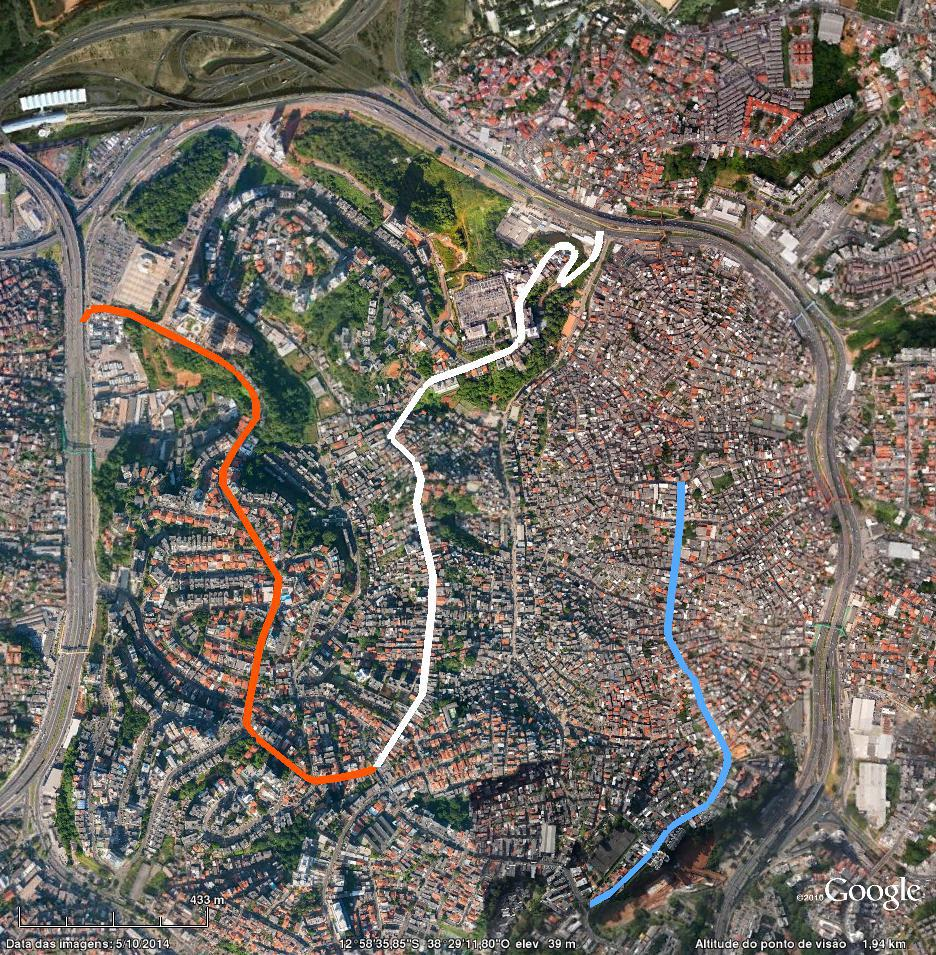
\includegraphics[width=0.7\textwidth]{3-cap2/complementos/mapas/matatu-hoje.eps} 
\label{fig:matatu-hoje}
 }
\caption{Duas representações cartográficas do Matatu, mostrando a rua da Valla (atual av. Heitor Dias), a Estrada da Pólvora (atual rua Raul Leite), a Estrada do Matatu Grande (atual rua Luiz Anselmo) e a Quinta das Beatas (atual Cosme de Farias).}
\end{figure}
 
No mesmo mapa é possível encontrar símbolos indicativos de construções pontilhando a cumeada do Matatu Grande, embora a cumeada onde se localiza a Casa da Pólvora apresente-se pouco povoada, assim como a da Quinta das Beatas. Novamente lendo o mapa de Weyll no sentido NNE-SSE (\autoref{fig:matatu-1851}), quatro rios escavam os vales circundantes destas cumeadas; todos já foram caracterizados na \autoref{subsec:pontnat} (p. \pageref{subsec:pontnat}). 

Dado o grande tamanho da área analisada, será preciso subdividi-la nos pontos notáveis e nomes pelos quais era conhecida na época, atualizando-os quando necessário.

\subsubsection{Quinta das Beatas: religião e latifúndio}\label{subsubsec:beatas}

Passado trecho da estrada das Pitangueiras, chega-se a uma esquina onde se abre a estrada que conduz à \textit{Quinta das Beatas}. A fazenda que ficou conhecida por este nome, no atual bairro de Cosme de Farias, tem sua descrição no \textbf{Livro Eclesial de Registro de Terras da Freguesia de Brotas} extremamente danificada pela ação do tempo:

\begin{citacao}
Quinta das Beatas

[\textit{ilegível}] fazenda denominada Quinta das Beatas é propriedade do Recolhimento do Senhor Bom Jesus dos [\textit{Perd}]oens, está situada na freguesia de Nossa Senhora [\textit{de}] Brotas, confina pelo nascente com a fazenda de[\textit{no}]minada Campina, dos herdeiros do coronel João Ladis[\textit{la}]u de Figueredo, e Matatu Grande, pertencente ao [\textit{José Antonio}] Pinto, pelo poente com a roça do tenente[\textit{-coron}]el Pinheiro e com o capitão Paranhos, pelo sul [\textit{com}] a roça de Amorim Vianna, com a Torre e com a [\textit{ilegível}] e pelo norte com o Matatu pequeno e com [\textit{ilegível}] [\textit{ilegível}] Paranhos. Bahia, dezesseis de março de [\textit{mil oitocentos e}] sessenta. Anna Maria Magdalena Re[\textit{jente}]. [\textit{E nada mais}] se continha em as ditas declarações [\textit{que me for}]am enviadas. Brotas da Bª, 20 de [\textit{março de 1860}]. Vigº Ernesto de Olivª Valle\footnote{\textbf{BR BAAPB}, fundo Colonial, série Registros de Terra, livro 4675, f. 40 verso.}.
\end{citacao}

A antiga sede da fazenda, a julgar pelo que mostra o mapa de \citeonline{weyll_mappa_1851}, estaria em algum lugar no trecho da atual rua Cosme de Farias situado entre as esquinas das atuais ruas Jaguarari e Lima Durval.

A relação entre o Recolhimento dos Perdões e a Quinta das Beatas é um dos mais acabados exemplos do \textit{rentismo}, sustentáculo econômico de tantas ordens religiosas católicas desde a fundação de Salvador até o presente. Veja-se o registro de uma fazenda foreira a Jacintho Muniz Barretto:

\begin{citacao}
Jacintho Muniz Barretto vae registrar a sua fazenda denominada Quinta das Beatas, foreira ao Recolhimento dos Perdoens, sita na freguesia de Brotas desta Capital, a qual divide com as [ilegível] seguintes: pelo lado do norte com os fundos das roças do Matatu Grande do Pinto, e com os do Matatu Pequeno, pertencente ao coronel Dom Braz Balthazar da Silveira ao Cabral e ao Capitão Paranhos, pelo do sul com os fundos da roça do Amorim, com as da fazenda da Torre e com as das roças de Antonio da Silva Quaresma [ilegível] [Joa]quim de Santa Thereza, pelo do leste [ilegível] [\textit{fundos}] da fazenda da Campina pequena pertencente aos herdeiros do Coronel João Ladislau de Figueiredo e Mello e também com as do Matatú Grande do Pinto, pelo do oeste com os fundos das roças do Tenente Coronel Joaquim da Costa Pinheiro, e também com as do Capitão Paranhos. Bahia, dezesseis de julho de mil oitocentos e cincoenta e nove. Jacintho Muniz Barretto. E nada mais continhão as declarações que me forão transmitidas. Brotas da Bª, 18 de julho de 1859. Vigº Ernesto de Oliveira Valle\footnote{\textbf{BR BAAPB}, fundo Colonial, série Registros de Terra, livro 4675, f. 39 verso.}.
\end{citacao}

Não se trata de aforamento pequeno, e sim de uma vasta herdade. Na tentativa de fazer subir sua ordem na hierarquia eclesial (de \textit{recolhimento} a \textit{casa de professas}), mais especificamente como parte da ordem das carmelitas calçadas, as irmãs recolhidas nos Perdões argumentaram por todos os meios possíveis, incluindo os econômicos; em 1820 alegaram possuir, além do 

\begin{citacao}
recato e honestidade em que vivião, o possuirem renda sufficiente de 28 predios urbanos, a grande roça de nossa Sra. da Conceição das Brotas, mais conhecida por \textit{quinta das beatas}, não pequena porção de terreno arrendado e aforado, além de 16:000\$000 rs. em dinheiro de varios legados [\dots] \cite[p.~231]{accioli_memorias5_1937}.
\end{citacao}

Embora o relato apresente mais uma das tentativas frustradas de ascensão hierárquica das recolhidas, deixou evidente seu poder econômico. Pequeno, se comparado ao dos beneditinos, por exemplo \cite{bento_tombo_1945}, mas, mesmo assim, \textit{poder}. 

\subsubsection{Matatu Grande e Matatu Pequeno: uma pequena África em Brotas?}\label{subsubsec:matatu}

Passada a entrada da Quinta das Beatas, a estrada das Pitangueiras segue adiante até surgir uma bifurcação entre a \textit{Estrada do Matatu Grande} (direita) e a \textit{Estrada do Matatu Pequeno} (esquerda)\footnote{Há indicação de que a Estrada do Matatu Grande corresponderia às atuais ruas Luiz Anselmo e Raul Leite, e a Estrada do Matatu Pequeno à atual rua Barros Falcão \cite[p.~124]{valladares_beaba_2012}; a indicação, entretanto, não faz sentido, porque a junção da Luiz Anselmo com a Raul Leite resultaria numa grande via, em forma aproximada de ``U'', que reuniria as cumeadas dos morros que no mapa de \citeonline{weyll_mappa_1851}, contemporâneo das antigas denominações, são separadas como ``Matatu Grande'', à direita, e ``Casa da Povora'', à esquerda. Na falta de documentos comprobatórios da mudança toponímica, não encontrados até onde foi possível avançar na pesquisa ora exposta, parece muito mais plausível que a Estrada do Matatu Grande corresponda à rua Luiz Anselmo e a Estrada do Matatu Pequeno à rua Raul Leite.}.

O \textit{Matatu Grande} situa-se ao final de uma estrada que corresponde em grande parte à atual Rua Luiz Anselmo. O \textbf{Livro Eclesial de Registro de Terras da Freguesia de Brotas} registra a existência de uma só fazenda chamada ``Matatu Grande'', registrada em nome de José Antonio Pinto, infelizmente ilegível\footnote{\textbf{BR BAAPB}, fundo Colonial, série Registros de Terra, livro 4675, ff. 28 verso e 29 frente.}. Sucessivos anúncios de venda de capim na ``fazenda Matatú Grande''\footnote{\textbf{Gazeta da Bahia}, várias edições entre 1879 e 1886.} parecem indicar tratar-se de uma só fazenda, mas o anúncio do leiloamento da roça de Bernardo Pires da Costa Chastinet, fiel da Tesouraria da Fazenda residente no Maciel de Baixo, demonstra o contrário:

\begin{citacao}
Uma roça e casa na estrada do Matatú Grande, na freguezia de Brotas, tendo quarenta metros e vinte centimetros de terreno de frente, e dentro três pés de mangueiras, três pés de jaqueiras, coqueiros, cajueiros, bananeiras, avaliado cada metro do terreno a cinco mil réis, e todos por duzentos e um mil réis. Os arvoredos todos avaliados em quarenta mil réis.

Uma casa terrea edificada na frente da estrada, e mede nove metros de frente, de paredes de taipa, tendo porta e duas janellas, estando do lado do norte parte da parede cahida; tem sala aberta e escorada, um quarto e cozinha com porta para o fundo, e toda a casa é feita da mesma construcção da frente, está toda coberta de telha, avaliada por sessenta mil réis; todo o terreno é proprio e divide pelo fundo com o rio Baixão que encosta as terras pertencentes ao proprietario Vidal de Oliveira, e pelo lado do norte com a roça de Thomé de Sant'Anna e pelo sul com terras de Miguel dos Anjos, sendo todo o terreno de ribanceira desde a frente até o brejo, avaliado tudo em tresentos e um mil réis\footnote{\textbf{O Monitor}, 25 fev. 1881, p. 2.}.
\end{citacao}

Meses depois, seria judicialmente arrematada uma ``rocinha com pequena casa de morar arruinada, avaliada em 301\$000'' penhorada a Bernardino Pires da Costa Chastinet por Antonio Ferreira Leal\footnote{\textbf{Gazeta da Bahia}, ano III, nº 162, 28 jul. 1881, p. 2.}; é possível que se trate da mesma propriedade. 

Outros anúncios coetâneos demonstram a existência de vários imóveis na área.

No \textit{Matatu Pequeno} o principal ponto de referência é a \textit{Casa da Pólvora}, descrita no mapa de \citeonline{weyll_mappa_1851} como ``Casa da Povora''; daí que a Estrada do Matatu Pequeno seja tratada, na documentação encontrada, também como \textit{Estrada da Pólvora}, ou \textit{Estrada da Casa da Pólvora}. Este ponto notável foi construído com base em portaria expedida em 1802 pelo governador e capitão-general da Capitania da Bahia, Francisco da Cunha e Meneses, ordenando ao capitão-de-mar-e-guerra, intendente da marinha e armazéns gerais, a construir uma ``casa de pólvora'' no sítio do Matatu \cite[p.~93]{oliveira_ultramar_1977}. A julgar pelo mapa de \citeonline{weyll_mappa_1851}, a Casa da Pólvora localizava-se no sítio onde hoje está a \textit{Vila Militar do Matatu}, administrada pelo Exército. 

Em 1868 a estrada da Casa da Pólvora foi consertada, pois seu mau estado de conservação arriscava explodir os barris de pólvora transportados, de tantos solavancos a que eram submetidos no transporte \cite[anexo~G,~p.~9]{bahia_anexosrelatorio_1868}. A Casa da Pólvora propriamente dita foi consertada em setembro de 1871 pelo pedreiro Estanisláo João da Cruz ao custo de 84\$348\footnote{\textbf{Jornal da Bahia}, ano XIX, 21 set. 1871, p. 1}; ainda funcionava em 1881 com a mesma finalidade de depósito de explosivos, como o demonstra um relatório indicando a saída de 60 barris de pólvora ``pertencente ao commercio'', com peso líquido de 683,5kg\footnote{\textbf{O Monitor}, 06 fev. 1881, p. 1.}, mas em 1888 já se dizia estar a Casa da Pólvora em ``logar muito improprio'' \cite[vol.~3,~p.~40]{bahia_relatorio_1888}. 

Ainda no mapa de \citeonline{weyll_mappa_1851}, a estrada da Casa da Pólvora abre para outros dois pequenos caminhos, correspondentes ao que hoje seriam as esquinas das ruas Laura Costa e Professor Osvaldo O'Dwyer, na Vila Laura. Estes curtos caminhos nem são nomeados nos mapas nem na documentação pesquisada nem na bibliografia consultada, pelo que é possível inferir que se trata de acessos a propriedades rurais tão-somente.

Caracteriza os dois Matatus a proliferação de \textit{pequenas posses}, inscritas no \textbf{Livro Eclesial de Registro de Terras da Freguesia de Brotas} por força da Lei 601/1850. A mais famosa entre elas talvez seja a de \textit{João Francisco Régis}, que por seis patacas anuais arrendou o terreno onde hoje se situa o \textit{terreiro do Alaketo}. Vistas as coisas pelo ponto de vista historiográfico, complementarmente ao ponto de vista mitológico exposto na \autoref{subsec:pontrel} (p. \pageref{subsec:pontrel}), há aspectos interessantíssimos na tradição do Alaketo, que merecem longa citação por extenso antes de comentários:

\begin{citacao}
Segundo as tradições orais de Ketu, das cento e vinte linhagens que se engajaram na migração, nove eram importantes famílias de Ifé, porém durante o período inicial de implantação no novo território quatro desapareceram sem deixar rastros, certamente dizimadas pelas guerras de adaptação, restando as cinco que até hoje se revezam no poder: Alapini, Magbo (pronuncia-se aproximadamente Magbô), Me1s1a (Mexá), Mefu e a nossa Aro. A linhagem Aro é portanto uma das famílias reais que fundaram o reino de Ketu e têm o direito constitucional de indicar por revezamento um candidato ao trono, eleito em seguida pelos \textit{oloyé}, membros do conselho de Estado. A segunda aldeia construída no novo território foi chamada de Aro, o que revela um destaque da linhagem homônima no ato da sua fundação, e tornou-se local sagrado nas tradições de Ketu, um dos espaços onde, através dos séculos, perfizeram-se os complexos ritos de entronização do Alaketu. Na aldeia de Aro encontra-se a tumba real do Alaketu Owé, o segundo rei de Ketu, certamente desta linhagem. Os Aro tiveram portanto um papel destacado na fundação do reino de Ketu há mais de mil anos, e alguns dos seus membros, em virtude das turbulências da história, vieram a encontrar-se, um belo dia, escravizados na Bahia. 

Os primeiros ataques do exército daomeano ao reino de Ketu deram-se em 1788 e 1789, em pleno reinado de Akibiohu, que durou de 1780 a 1795. Durante esta campanha os daomeanos saquearam inicialmente algumas fazendas e aldeias, dentre as quais Krukruhuntó. Em uma segunda investida, não conseguindo penetrar na capital — defendida por uma dupla muralha e ostentando a famosa porta Idena, o mais brilhante exemplo da arquitetura militar nagô-iorubana — prosseguiram sua devastação avançando mais para o sertão. [\dots] Segundo os historiadores do reino de Ketu, neste último ataque de janeiro de 1789 o exército daomeano saqueou e destruiu a cidade de Iwoye (Iuó-iê), situada alguns quilômetros ao norte de Aro e cerca de vinte e cinco quilômetros a nordeste da capital, perto da fronteira do reino de Shabé, já na região das savanas que precedem o deserto do Saara. A cidade de Iwoye era um importante centro litúrgico regional, mesmo o alaketu não poderia ordenar a prisão de um perseguido político que ali pedisse asilo, e parece ter sido um reduto da família Aro; a mãe do alaketo Akibiohu era natural daquela cidade, Ojeku, o pai das gêmeas seqüestradas, bem como sua família, certamente moravam lá. Em resumo, a linhagem (ou o clã) Aro parece ter sido responsável ritual e militar pela região nordeste do reino, onde a cidade de Iwoye e a aldeia de Aro eram os centros mais importantes. [\dots]

A fundadora do terreiro do Alaketo, Otampê Ojarô, seqüestrada aos nove anos de idade em janeiro de 1789, deve muito provavelmente ter nascido em 1779, deve ter levado nove anos no cativeiro e alforriada com a idade de dezoito primaveras nos ultimíssimos anos do século XVIII, digamos em 1798, voltando em seguida ao reino de Ketu. [\dots] Otampê Ojarô casou-se em Ketu, segundo a tradição oral do Alaketo, aos vinte e dois anos, admitamos que em 1801, e deve ter voltado logo em seguida ao Brasil, porque sua primeira filha, Akobiodé, era crioula, já nasceu na Bahia. Sabemos que a cultura africana em geral atribui imenso valor à progenitura e, em situações normais, um casal estabelecido logo tem um filho, o qual representa a consumação do casamento. Este dado indica a provável presença da comitiva da família Aro, encabeçada por Babá Láji, Otampê Ojarô e Obokô Mixôbi, na Bahia, nos primeiríssimos anos do século XIX, digamos por volta de 1802. Otampê Ojarô devia estar portanto, nesta data, residindo na Bahia, grávida de Akobiodé e ritualisticamente preparada para fundar uma casa do culto nagô-vodum.

O foco no início do século XIX parece também ser corroborado pela conhecida certidão de 1858, o mais antigo documento oficial do Alaketo. Este documento não se refere ao arrendamento das terras do Matatu Grande, como muitos crêem, apenas atesta que neste momento o terreno já pertence ao neto de João Porfírio Régis, João Francisco Régis, filho primogênito de sua filha Iyá Akobiodé, falecido em 1867, sem especificar contudo se ele é possuidor ou proprietário\footnote{Como visto na \autoref{subsec:cidbraref} (p. \pageref{subsec:cidbraref}), trata-se do \textit{registro do vigário}, indicativo apenas da \textit{posse}.}. [\dots] Se, em 1858, o terreno pertencia ao neto do casal que inicialmente o obteve, tudo aponta para a concomitante obtenção das terras da Barroquinha e do Matatu Grande, por volta de 1807, 1808. [\dots] Quando, entre 1807 e 1808, os dois terrenos devem ter sido arrendados, o clima era de tensão na comunidade africana da Bahia. Babá Láji e Iyá Otampê Ojarô, nesta conjuntura, estavam decididos, primeiro, a obter um terreno distante do centro da cidade, e, segundo, a fundar um templo consagrado a Oxumarê, não a Airá Intile ou um outro orixá qualquer. [\dots] É provável que os membros da família Régis tenham discordado da opção pela Barroquinha por causa da proximidade do mosteiro de São Bento, do palácio dos governadores e do solar do Berquó, o qual era, na virada do século XVIII para o XIX, residência de um dos desembargadores do Tribunal da Relação. Esta promiscuidade com algumas das instituições centrais do Estado e com a moradia de um dos poderosos da Bahia colonial pode tê-los levado a procurar uma alternativa mais segura, em um momento de violência antiafricana. [\dots]

Além da distância do centro urbano, uma outra vantagem da Estrada do Matatu Grande era a concentração de africanos e casas de candomblé pelas suas cercanias. Segundo a documentação antiga do Alaketo, o terreno, pelos fundos, limitava-se com a Quinta das Beatas, reduto de casas de culto angolanas e congolesas de implantação mais antiga. Segundo as tradições orais, existia na Quinta das Beatas um cemitério angolano onde se realizava o culto de Tempo Kiamuilo, e, ao longo do século XIX, os tapás e nagô-iorubás foram se instalando pelas vizinhanças, com destaque para os cultos de Orixá Okô e dos ancestrais Babá Gunukô e sua esposa Abakô Laí, no local onde hoje se encontra a Avenida Bonocô. O terreiro do Alaketo deve ter sido o primeiro candomblé nagô a instalar-se na região. [\dots] Distantes do centro, os membros da família Régis tomaram posse de um terreno fértil, com três fontes de águas límpidas, onde plantaram fundamentos trazidos da África, transformando-o em um terreiro de Oxóssi; aí plantaram algumas árvores sagradas, dois pés de biriba que já “morreram de velho”, entre os quais foi assentado Obá Unlu, “o primeiro Oxóssi”, antigo rei-caçador divinizado; plantaram também um iroko (gameleira branca), do qual nasceu um outro, que hoje, gigantesco, domina a região; plantaram hortas e árvores frutíferas de várias espécies, preparando-se para viver sem privações. No centro do terreiro construíram um barracão de taipa, ``com trinta e oito palmos de frente'', o ilê Maroiá Láji, templo dedicado a Oxumarê, além de outras edificações menores para o funcionamento do novo culto.

Tudo indica portanto que o final do governo do conde da Ponte foi o momento do desfecho da cisão, e o início do governo do conde dos Arcos o momento de colocação das bases de duas distintas trajetórias para os dois terreiros de Keto mais antigos da Bahia. Desde esta pri-
meira cisão, o Alaketo permaneceu um candomblé do povo de Ketu, mais precisamente, da linhagem Aro e seus aliados, ou, melhor ainda, da família Régis “pela parte do Brasil”, enquanto que, na Barroquinha, começava um processo de abertura com grandes desdobramentos posteriores, onde jejes e ketus se associariam a outros subgrupos étnicos provenientes de várias áreas do território nagô-iorubá, entre outros, os oyós, ijexás, egbás, ijebus, efans, que começaram a chegar à Bahia em grande número, a partir da década de 1820, trazendo novas tradições litúrgicas que se incorporariam às tradições baianas.

Na década de 1830 haveria na Barroquinha uma grande reestruturação, que associaria sacerdócios e divindades diversas em um só corpo político-religioso, sob a direção de Iyá Nassô, autoridade do primeiro escalão do declinante império de Oyó. E na década de 1850, época de predomínio na Bahia do grupo político do intolerante Visconde de São Lourenço, os nagôs seriam expulsos da Barroquinha quando da sua urbanização, sendo o candomblé invadido e profanado, instalando-se alguns anos depois no Engenho Velho da Federação, onde até hoje se encontra. Enquanto isso o Alaketo, desde a década de 1810, já havia encontrado seu lugar na estrada do Matatu Grande, onde se estabeleceu para durar séculos \cite[p.~354-356, 369-377]{silveira_alaketo_2003}.
\end{citacao}

A este fascinante relato deve-se somar, ressaltando-o, o fato de que trata-se de \textit{uma} entre as \textit{cinquenta} posses registradas nos dois Matatus (de um total de 141 posses registradas no \textbf{Livro Eclesial de Registro de Terras da Freguesia de Brotas} -- 35,46\% do total). Comparativamente, a segunda área com maior número de registros, o Acupe, tem apenas \textit{dezessete} registros, e a Quinta das Beatas, sua vizinha imediata, contém apenas \textit{três} registros. Esta proliferação de posseiros, quando cruzada com as reclamações na imprensa sobre quilombos, batuques, refúgio a escravos fugidos etc. (cf. \autoref{subsec:refugioescrav}, p. \pageref{subsec:refugioescrav}), leva à seguinte hipótese: trata-se de posses de \textit{libertos}, ao que tudo indica. Não basta, para o uso do espaço para fins proibidos por lei, ser ele distante, ermo, misterioso; é preciso contar também, em especial no caso dos usos mencionados, com uma \textit{rede de suporte e apoio}. A proliferação de posses no Matatu parece coerente com esta necessidade, pois trata-se não apenas de posses numerosas, mas de posses de pequenas dimensões, compatíveis com os rendimentos da pequena agricultura de subsistência, em se tratando de posses de terras arrendadas, ou com a pequena capacidade de poupança numa sociedade onde mesmo ao liberto apresentavam-se pouquíssimas, raríssimas e escassíssimas oportunidades de acumulação do capital necessário para investimento num bem que, no regime de terras então vigente, valia mais pelo poder que conferia e menos pelo seu valor econômico. É lícito, portanto, e ainda mais com os elementos a serem apresentados na \autoref{subsec:refugioescrav} (p. \pageref{subsec:refugioescrav}), suscitar a hipótese de que os dois Matatus compunham uma ``pequena África'' inserida no território soteropolitano, hipótese ainda mais reforçada ao saber-se que em 1849 estavam em Brotas 232 libertos africanos, dos quais 90\% dos homens se dedicavam à agricultura \cite[p.~151]{COSTA1989}.

A situação no Matatu lança luzes interessantes também sobre a questão do registro de terras posterior à Lei 601/1850. Teriam os pequenos posseiros do Matatu, em seguida à promulgação da Lei de Terras, acorrido ao vigário de Brotas para garantir o registro de suas posses? Tudo indica que sim. Seriam estes \textit{todos} os posseiros da freguesia? Somente um escrutínio rigoroso da imprensa da época, comparado aos registros do \textbf{Livro Eclesial de Registro de Terras da Freguesia de Brotas}, poderia talvez dizê-lo -- escrutínio este que ultrapassa o escopo da pesquisa fundamentadora desta dissertação. É licito, apesar disto, suscitar a hipótese de que os posseiros das pequenas herdades periurbanas de Salvador, diante da promulgação da Lei de Terras, acorreram aos vigários para garantir suas posses antes que as perdessem por falta de registro.

\subsection{A fazenda Torre e os remanescentes da fazenda Acupe}

A Casa da Torre possuía no século XVIII uma roça na região hoje conhecida como \textit{Acupe de Brotas}, que a viúva de Garcia d'Ávila Pereira vendeu em 1765 por 500\$000 \cite[p.~10]{ott_engenhos_1996}. É muito provável ser esta a roça conhecida como ``Torre'', cujo registro no \textbf{Livro Eclesial de Registro de Terras da Freguesia de Brotas} anda bem danificado:

\begin{citacao}
Roça da Torre

Vem o abaixo assignado [\textit{ilegível}] [\textit{ilegível}] [\textit{uma linha inteira ilegível}] [\textit{ilegível}]ada Roça da Torre [\textit{ilegível}] [\textit{duze}]ntas e vinte e seis braças, limitandose pelo [\textit{ilegível}] da Cidade com a roça da viúva Amorim [\textit{ilegível}] lado das Brotas com a roça do finado [\textit{Mem}] de Amorim [\textit{Filgu}]eiras e pelo fundo com a [\textit{Q}]uinta das Beatas. Bahia, oito de março de [\textit{mil}] oitocentos e sessenta. Francisco Pires de [\textit{Carv}]alho Albuquerque. E nada mais [\textit{ilegível}]tinha em as declarações que me foram [\textit{ilegível}]. Brotas da Bª, 17 de março de [1860]. Vigº Ernesto de Olivª Valle\footnote{\textbf{BR BAAPB}, fundo Colonial, série Registros de Terra, livro 4675, f. 40.}
\end{citacao}

O jornal \textbf{Idade d'Ouro do Brazil} anunciou, em julho de 1817, que Victorino dos Santos Pereira -- dono de muitas outras coisas expostas no mesmo anúncio\footnote{O sr. Victorino aparentava ser comerciante, pois anunciou no \textbf{Idade d'Ouro do Brazil} vender ``breu de muito boa qualidade'', ``alcatrão d'América'', ``cabos sortidos'', lonas ``da Suécia'' e ``da Rússia'', ferro ``redondo'' e ``em barra'', pregos e aço. Além disso, Victorino Pereira aparentava ser muito bem provido de bens, pois ``não duvida vender a dinheiro, ou com prazo, um barco de 66 palmos de quilha muito bem construido''; se o comprador quisesse, ainda poderia ``comprar o Mestre e quatro Marinheiros escravos''. Reforça esta impressão o fato de vender também, no mesmo anuncio, vários sitios e fazendas: \textit{Murici}, em Itapicuru, com duas léguas; \textit{Rio de Paus}; a fazenda \textit{Ramalho}, no distrito de Carinhanha, ``Termo da Vila de Jacobina''; as fazendas \textit{Riacho} e \textit{Porto de João Pereira}, no Rio Preto; no Lagarto, as fazendas \textit{Curral Novo}, ``\textit{Ingola caxorro}'', \textit{Palma} e \textit{Pé de Serra}, alem dos sitios \textit{Macuna}, \textit{Tapeirinha} e \textit{Piauí}, ``próprios para criar gado'' (\textbf{Idade d'Ouro do Brazil}, nº 55, 15 jul. 1817, p. 4).} -- prometia a recompensa de dez mil-reis para quem encontrasse ``um cavalo ruço queimado de bom tamanho marca DM na pata direita, assendeirado cauda curta, crina sem estar aparada'' \footnote{\textbf{Idade d'Ouro do Brazil}, nº 55, 15 jul. 1817, p. 4}. O cavalo pertencia aos bens da roça \textit{Torre}, que o abastado sr. Victorino dizia ser de sua propriedade.

\begin{figure}[!htp]
\centering
\includegraphics[width=1\textwidth]{3-cap2/complementos/mapas/georreferenciamento/acupe/acupe-1851.eps}{\footnotesize \par \textbf{Fonte:} \citeonline{weyll_mappa_1851}. \par}
\label{fig:acupe1851}
\caption{Representação cartográfica parcial das fazendas Torre e Acupe (1851)}
\end{figure}

\begin{sidewaysfigure}[!htp]
\centering
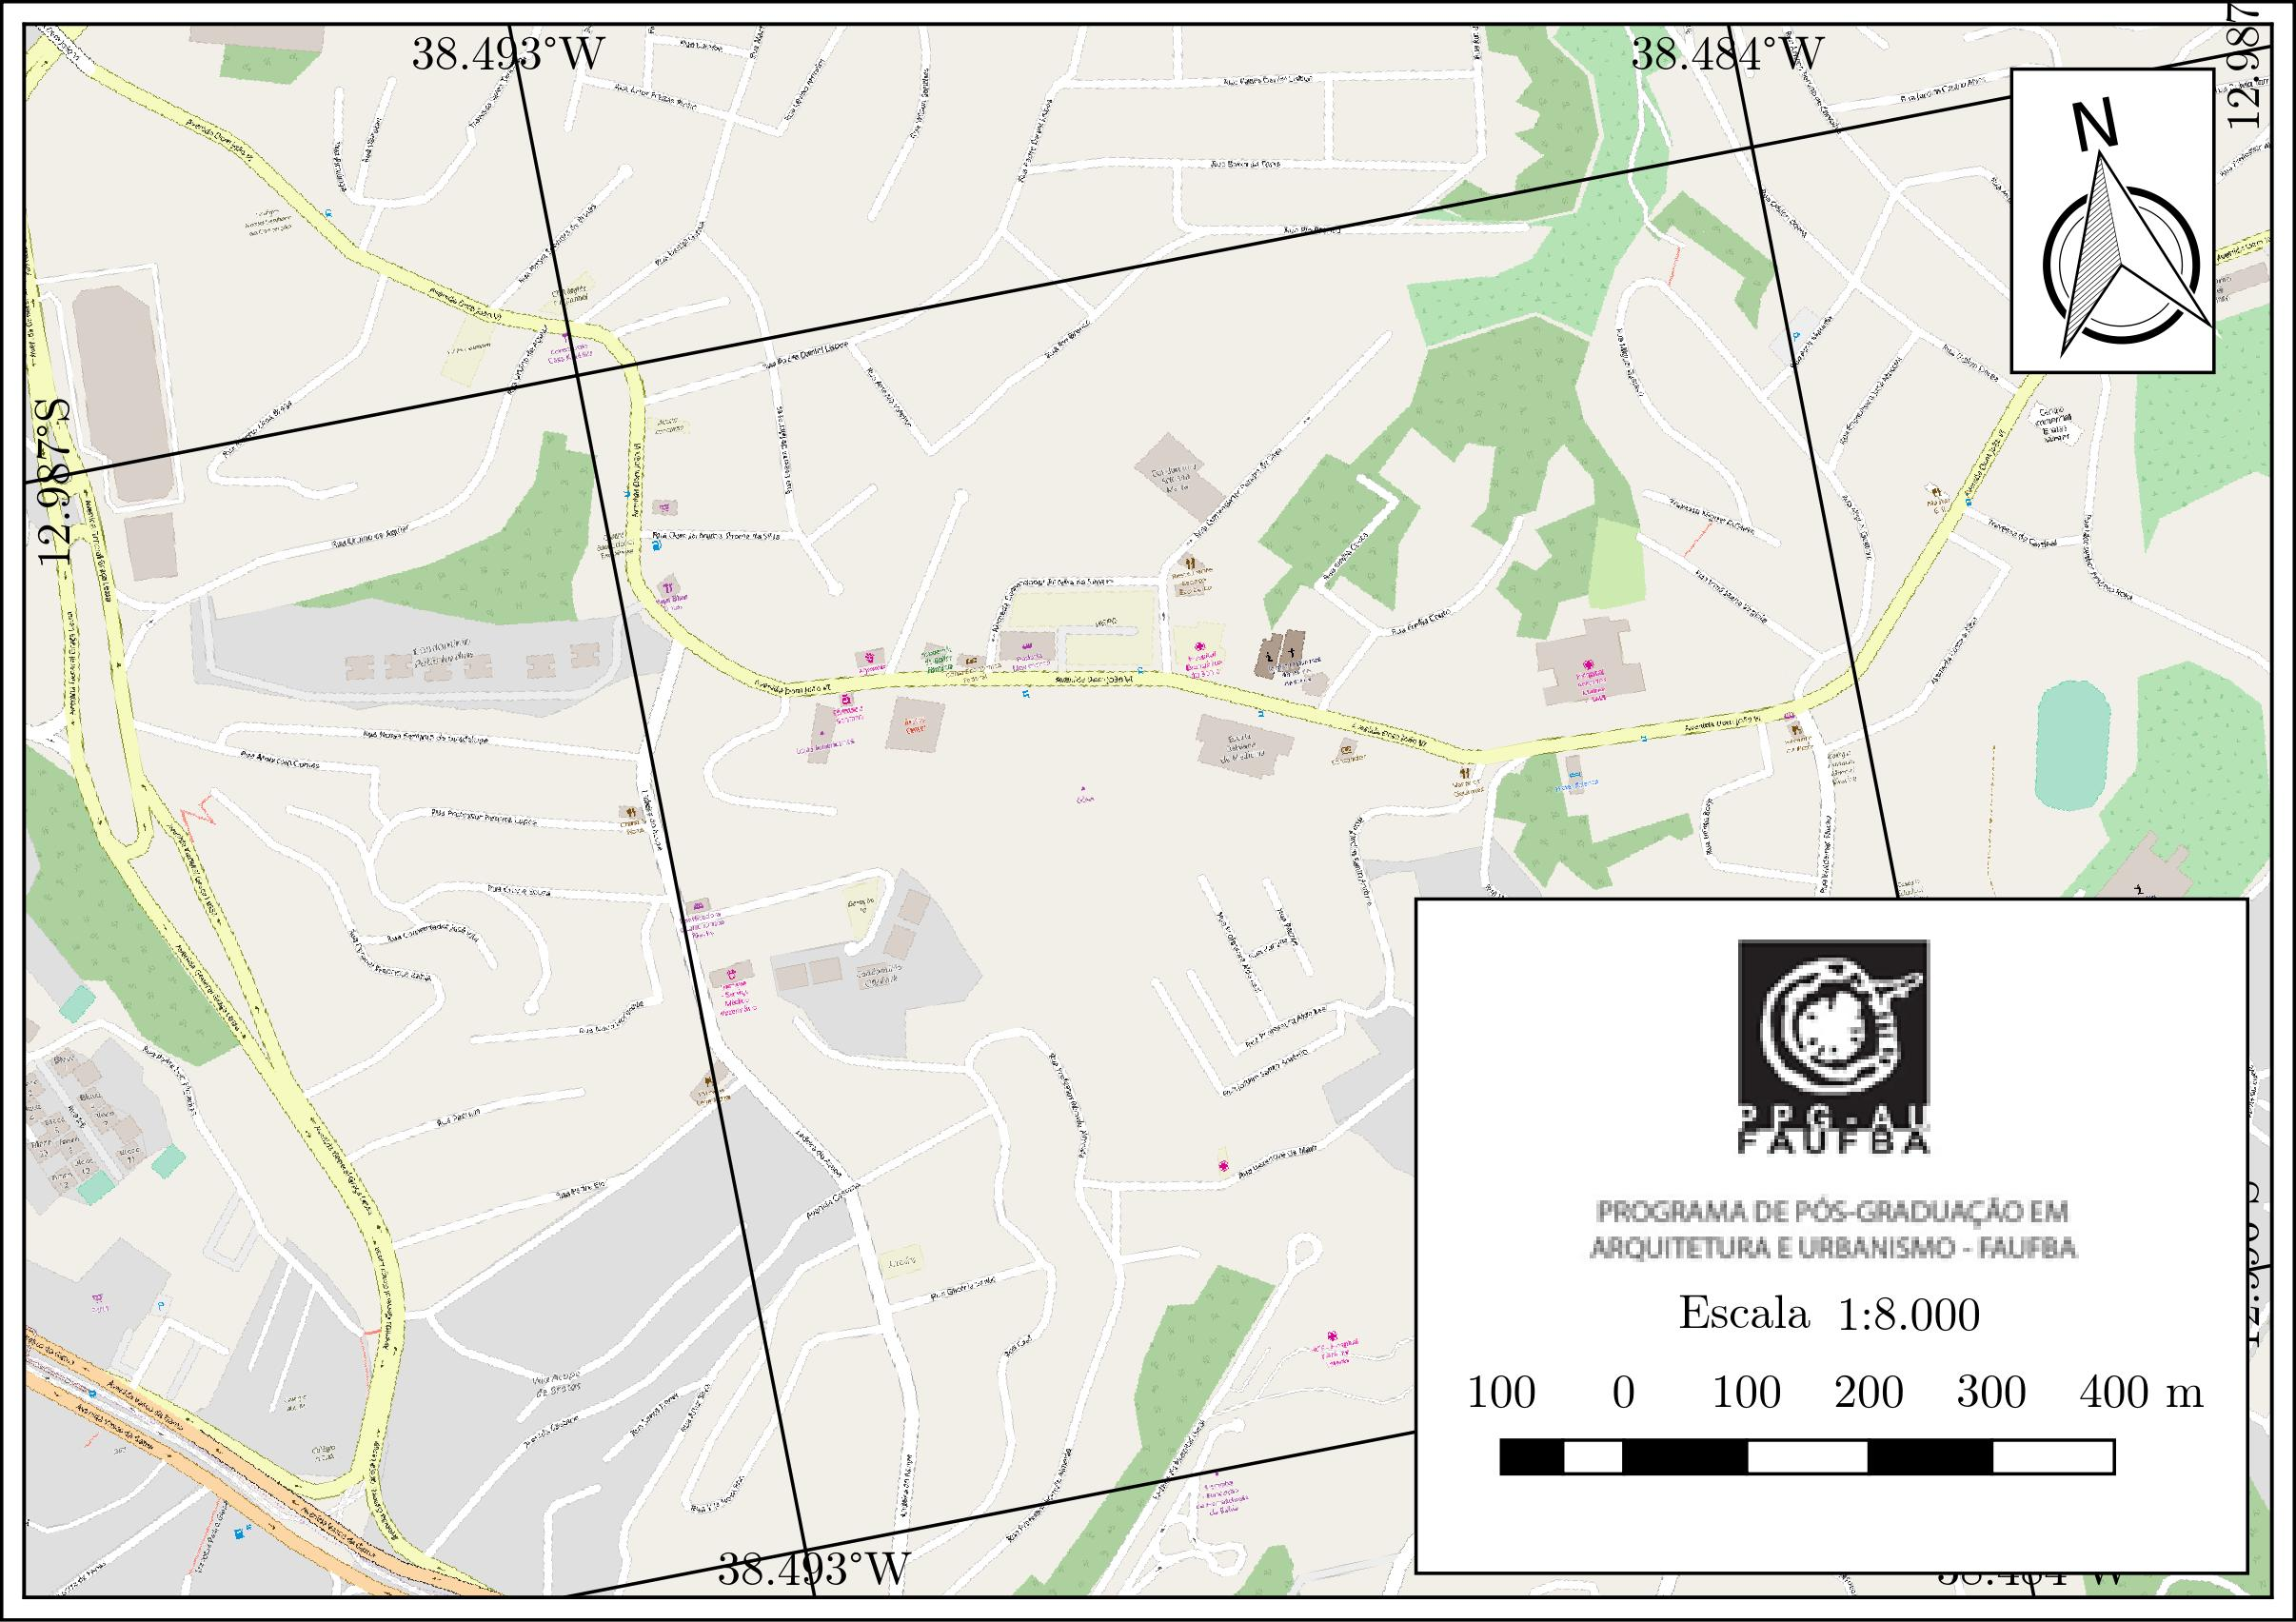
\includegraphics[width=0.8\textwidth]{3-cap2/complementos/mapas/georreferenciamento/acupe/acupe-2016.eps}{\footnotesize \par \textbf{Fonte:} Elaboração do autor com imagem do Open Street Maps. Respeitou-se o traçado de \citeonline{weyll_mappa_1851}. \par}
\caption{Representação cartográfica parcial da av. D. João VI e da ladeira do Acupe}
\label{fig:acupe2016}
\end{sidewaysfigure}

Ainda em 1877 existia a fazenda Torre, pois no dia 10 de janeiro do mesmo ano foi encontrado um cadáver em estado de putrefação num ``brejo de plantado de capim'' nela situado\footnote{\textbf{O Monitor}, 13 jan. 1877, p. 1.}. Em 1879 foi anunciado o aluguel de ``chácara, com grande roça'', que pertencera à fazenda Torre, ``grande plantação de capim, porção de terreno proprio para qualquer plantação, excellente agua potavel, bom banho, em logar muito pitoresco e saudavel e assim uma outra casa menor no mesmo terreno''\footnote{\textbf{O Monitor}, 23 jan. 1879, p. 2.}.

Já a fazenda Acupe está já dividida no \textbf{Livro Eclesial de Registro de Terras da Freguesia de Brotas}, como se vê:

\begin{citacao}
Dona Maria da Piedade Tabirá Bahiense, viúva do Coronel Antonio Lopes Tabirá Bahiense, possui um terreno no lugar denominado Acupe, na freguesia de Nossa Senhora das Brotas desta Capital, com sete braças de frente linha recta, segundo sua escriptura, que dá para a mesma estrada. Esta roça outrora foi parte da fazenda denominada Acupe e como pertencesse a diversos esses venderam suas partes, teve de fazer-se uma estrada pelo centro, e veio a tornarse a frente em uma linha diagonal contendo doze braças de frente, por que em uma das extremidades faz um funil, confinando por um lado com a roça de Elias Lopes de São Jerônimo, linha recta da pedra marca do rego mestre e por elle acima até encontrar com terras da roça de dona Maria Rosa Gomes da Silva, seguindo-se outra recta da valla que desce da estrada do Engenho Velho, atravessando o rego mestre até a estrada do Acupe, onde teve princípio esta demarcação, e pelo fundo com Barnabé Arraes, pelo mesmo rego mestre. Bahia, primeiro de junho de mil oitocentos e cincoenta e oito. Dona Maria da Piedade Tabirá Bahiense. E nada mais continhão as declarações que me forão enviadas. Brotas da Bª, 21 de junho de 1858. Vigº Ernesto de Olivª Valle\footnote{\textbf{BR BAAPB}, fundo Colonial, série Registros de Terra, livro 4675, f. 11.}
\end{citacao}

No mapa de \citeonline{weyll_mappa_1851} já se vê a referida estrada, donde se deduz que a divisão da fazenda Acupe se deu bem antes do seu registro. A região permaneceu eminentemente agrícola por todo o século XIX. Sobre o assunto, veja-se, primeiramente, um anúncio de 1839:

\begin{citacao}
Quem quizer comprar as benfeitorias d'umma excellente roça, no sitio denominado Acú Pequeno, na estrada de Brotas, contendo a plantação seguinte: 2400 e tantos pés de larangeiras de diversas qualidades todos dando fructo, 200 á 300 ditos de coqueiros, 200 e tantos ditos de jaqueiras, 300 e tantos ditos de mangueiras, e cento e tantos pés de craveiros da India, dando; assim como limoeiros dôces e azedos em grande quantidade, limeiras da Persia e de embigo; um brejo com todas as qualidades de ortaliça, grande bananal, e bastante capim plantado, e outras muitas coisas que se não faz menção, a qual tem boa casa de vivenda, e de fazer farinha, estribaria para cavallos, e curral para vaccas de leite, achando-se livre e desembargada de qualquer ônus [\dots]\footnote{\textbf{Correio mercantil}, ano 4, º 275, 24 dez. 1839, p. 3.}.
\end{citacao}

Em seguida, veja-se o seguinte anúncio, de 1876:

\begin{citacao}
ROÇA

Aluga-se na estrada de Brotas, lugar denominado Acú, uma roça com casa de morar, arvoredos frutiferos, boa fonte de bica, brejo para plantação. Quem a pretender dirija-se a venda do beco que achará com quem tratar\footnote{\textbf{Diário de Notícias}, ano 2, nº 199, 02 set. 1876, p. 3}.
\end{citacao}

Em 1872 o governo provincial, tendo em vista que o cemitério de Brotas não funcionava já fazia quatro meses por não haver mais ``logar para as inhumações'', ``mandou por em arrematação pela [\textit{inspetoria}] de obras públicas a construcção de um novo cemiterio para aquella localidade no logar denominado `Acú''', escolhida ``por ser [\dots] no centro da freguezia'' e, por isto, reduzir as despesas funerárias de seus moradores \cite[p.~12]{bahia_1872}. A totalidade dos documentos pesquisados demonstra, entretanto, que um tal cemitério nunca foi construído, e que o cemitério de Brotas voltou a seu funcionamento regular.

Além de área agrícola, o Acupe é área de persistente presença africana. Tornou-se famoso o caso da invasão polícial em 1829 a um terreiro ali existente, a mando do juiz de paz Antonio Gomes de Abreu Guimarães \cite[pp.~32-61]{REISSILVA1989}; menos conhecida, entretanto, é a continuidade dos ``batuques'' e ``calundus'' na área trinta e cinco anos depois, desta vez ``na roça de uma senhora Marocas, sob a direção de um africano de nome Domingos'' \cite[p.~137]{reis_domingos_2008}; sendo ``Marocas'' um apelido de ``Maria'', o \textbf{Livro Eclesial de Registro de Terras da Freguesia de Brotas} fornece o nome de pelo menos cinco ``candidatas''\footnote{Eliminadas Maria da Piedade Tabirá Bahiense e Maria Rosa Gomes da Silva (a esta altura já falecida), restam, nomeadamente: \textit{Maria} Francisca de Santana, \textit{Maria} Amélia de Carvalho Martagão, \textit{Maria} Constança Ebé, Thimothea \textit{Maria} Lopes, Rosa \textit{Maria} do Amor Divino.}, das quais a mais provável é Maria Constança Ebé:

\begin{citacao}
Roça de D. Maria Constança Ebé

Roça sita no Acu, freguesia de Nossa Senhora das Brotas, com casa abarracada, terreno proprio, com vinte e duas braças de frente e cincoenta e quatro de fundo, dividindo este [ilegível] [ilegível] [ilegível] e os herdeiros de Vasco Carneiro de [ilegível] pela frente e pelo sul com a roça do falecido Doutor Salustiano José Pedrosa, e pelo norte com a de Caetana Roza da Conceição. Bahia, dezesseis de julho de mil oitocentos e cincoenta e oito. Por Maria Constança Ebé, Pedro Alves Barbosa. E nada mais continhão as declarações que me foram enviadas. Brotas da Bª, 17 de julho de 1858. Vigº. Ernesto de Olivª Valle\footnote{\textbf{BR BAAPB}, fundo Colonial, série Registros de Terra, livro 4675, f. 33 frente.}.

Às vésperas da proclamação da república, a ladeira do Acupe ainda passava por melhoramentos, como o ``abahulamento e [...] abertura de alveos laterais em toda sua extensão'' ordenada pelo presidente da Câmara Municipal no expediente dos dias 11 a 19 de agosto de 1889 ao inspetor municipal de obras públicas\footnote{\textbf{Diário da Bahia}, ano 35, nº 247, 5 nov. 1889, p. 1.}.

\end{citacao}

\subsection{O Engenho Campinas: herdades e negócios de família}\label{subsec:campinasladislau}

\begin{figure}[!htp]
\centering
\subfloat[Em 1851. \textbf{Fonte:} elaboração do autor, com base em  \citeonline{weyll_mappa_1851}.]{
\includegraphics[width=0.7\textwidth]{3-cap2/complementos/mapas/campinas-1851.eps} 
\label{fig:campinas-1851}
 }
\  %espaco separador
\subfloat[Atualmente. \textbf{Fonte:} elaboração do autor, com base em imagem do Google Earth.] {
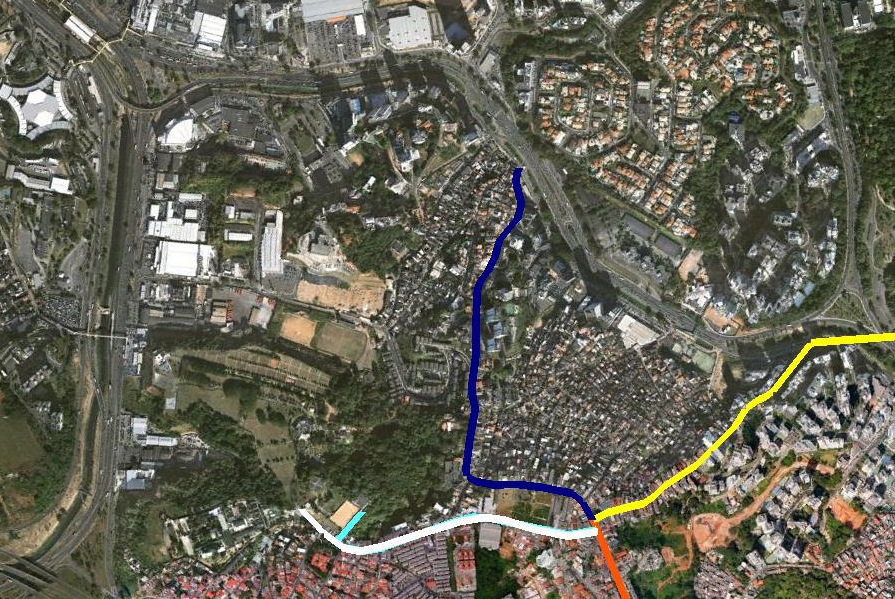
\includegraphics[width=0.7\textwidth]{3-cap2/complementos/mapas/campinas-hoje.eps} 
\label{fig:campinas-hoje}
 }
\caption{Duas representações cartográficas parciais do território correspondente às terras dos Ladislau.}
\end{figure}

Toda a área que hoje conhecemos como \textit{Campinas de Brotas} era, no século XIX, de propriedade de integrantes da família \textit{Ladislau de Figueiredo e Melo}, cujo patriarca, \textit{João Ladislau de Figueiredo e Melo}, veterano das lutas pela independência na Bahia e verdadeiro potentado local \cite[p.~59]{REISSILVA1989}\footnote{Natural de Cachoeira e filho de Leandro de Figueiredo e Anna Maria Barbosa de Mello, João Ladislau de Figueiredo e Melo era proprietário ao morrer, além do engenho Campina Grande a ser visto mais pormenorizadamente, de uma fazenda na cidade de Cairu; de um engenho em Abrantes conhecido como ``Cagi'' (muito provavelmente originador da localidade do \textit{Caji}, em Camaçari); de trinta e cinco escravos nominados e distribuídos aos herdeiros arrolados, três outros alforriados e de outros tantos não individuados; de casas na Cruz da Redenção (esta deixada a sua filha Rosa, cuja fortuna será vista em momento oportuno), rua das Verônicas e ladeira de São Francisco; além de larga soma em dinheiro (apesar de declarar em testamento que ``não deixo dinheiro''), tudo distribuído \textit{ab intestato} entre filhos, netos, afilhados e bisnetos. \textbf{BR BAAPB}, fundo Judiciário, seção Inventários, estante 1, caixa 98, maço 143, documento 3.}, vinha a ser avô do mesmo \textit{José Álvares do Amaral} reivindicante da fazenda Alagôa. O próprio nome da área -- Campinas -- deriva de duas das herdades da família.

A primeira delas era a fazenda Campina Grande:

\begin{citacao}
Fazenda Campina Grande

Rosa Ladislau de Figueredo e Melo e Virgínia Ladislau de Figueredo e Melo possuem em condomínio nesta Freguesia de Nossa Senhora das Brotas uma Fazenda denominada Campina Grande, em que há Engenho de fabricar assucar, e que comprehende a fazenda do mesmo nome Campina Grande, [ilegível] Carregado e Chacôco, terras proprias, que de [ilegível] [ilegível] um lado com a roça da dita Rosa Ladislau de Figueredo e Melo no lugar da Cruz da Redempção e com outra denominada Campina Pequena de dona Michelina Ladislau e Silva e dona Joanna Fausta Ladislau e Silva, de outro com terras do Matatu de José Antonio Pinto pelo riacho de mesmo nome, e mais com terras do Girão de Joaquim Caetano de Almeida Couto, ou quem mais direito for, pelo riacho Camorogipe, outra com terras que forão de dona Maria de Argôlo, e com as do Engenho Santo Antônio da Viscondessa do Rio Vermelho e sua filha dona Judith Constança da Cunha, pelo dito Camorogipe, e pelo outro com a estrada que sobe da ponte do mesmo Camorogipe e com terras que forão de João Paulo e seu irmão Fabião. Esta declaração vae por uma de nós feita e por ambas assignada. Bahia e Freguesia de Nossa Senhora das Brotas, primeiro de junho de mil oitocentos e cincoenta e oito. Rosa Ladislau de Figueredo e Melo, Virgínia Ladislau de Figueredo e Melo. E nada mais continhão as declarações que me foram enviadas. Brotas da Bª, 5 de junho de 1858. Vigº Ernesto de Olivª Valle\footnote{\textbf{BR BAAPB}, fundo Colonial, série Registros de Terra, livro 4675, f. 4 verso e 5.}
\end{citacao}

A outra, a fazenda Campina Pequena:

\begin{citacao}
Roça Campina Pequena

Michelina Ladislau e Silva e Joanna Fausta Ladislau e Silva possuem nesta Freguesia de Nossa Senhora das Brotas uma roça denominada Campina Pequena com casa de vivenda e outras benfeitorias, terras próprias, e que se divide pela frente com terras de Raphael e José Joaquim, e por outro lado com a Quinta das Beatas pelo riacho que a separa, por outro com a estrada que entra para o Engenho da Campina Grande, e pelo fundo com terras do mesmo Engenho. Esta declaração vae feita por uma de nós e por ambas assignada. Bahia e Freguesia de Nossa Senhora das Brotas, primeiro de junho de mil oitocentos e cincoenta e oito. Michelina Ladislau e Silva, Joanna Fausta Ladislau e Silva. E nada mais continhão as declarações que me forão enviadas. Brotas da Bahia, 4 de junho de 1858. Vigº Ernesto de Olivª Valle\footnote{\textbf{BR BAAPB}, fundo Colonial, série Registros de Terra, livro 4675, f. 5 e 5 verso.}
\end{citacao}

\begin{sidewaysfigure}[!htp]
\centering
\includegraphics[width=0.8\textwidth]{3-cap2/complementos/mapas/georreferenciamento/campinas/campinas-1851.eps}{\footnotesize \par \textbf{Fonte:} \citeonline{weyll_mappa_1851}. \par}
\label{fig:campinas1851}
\caption{Representação cartográfica parcial das fazendas Campina Grande e Campinas Pequena.}
\end{sidewaysfigure}

\begin{sidewaysfigure}[!htp]
\centering
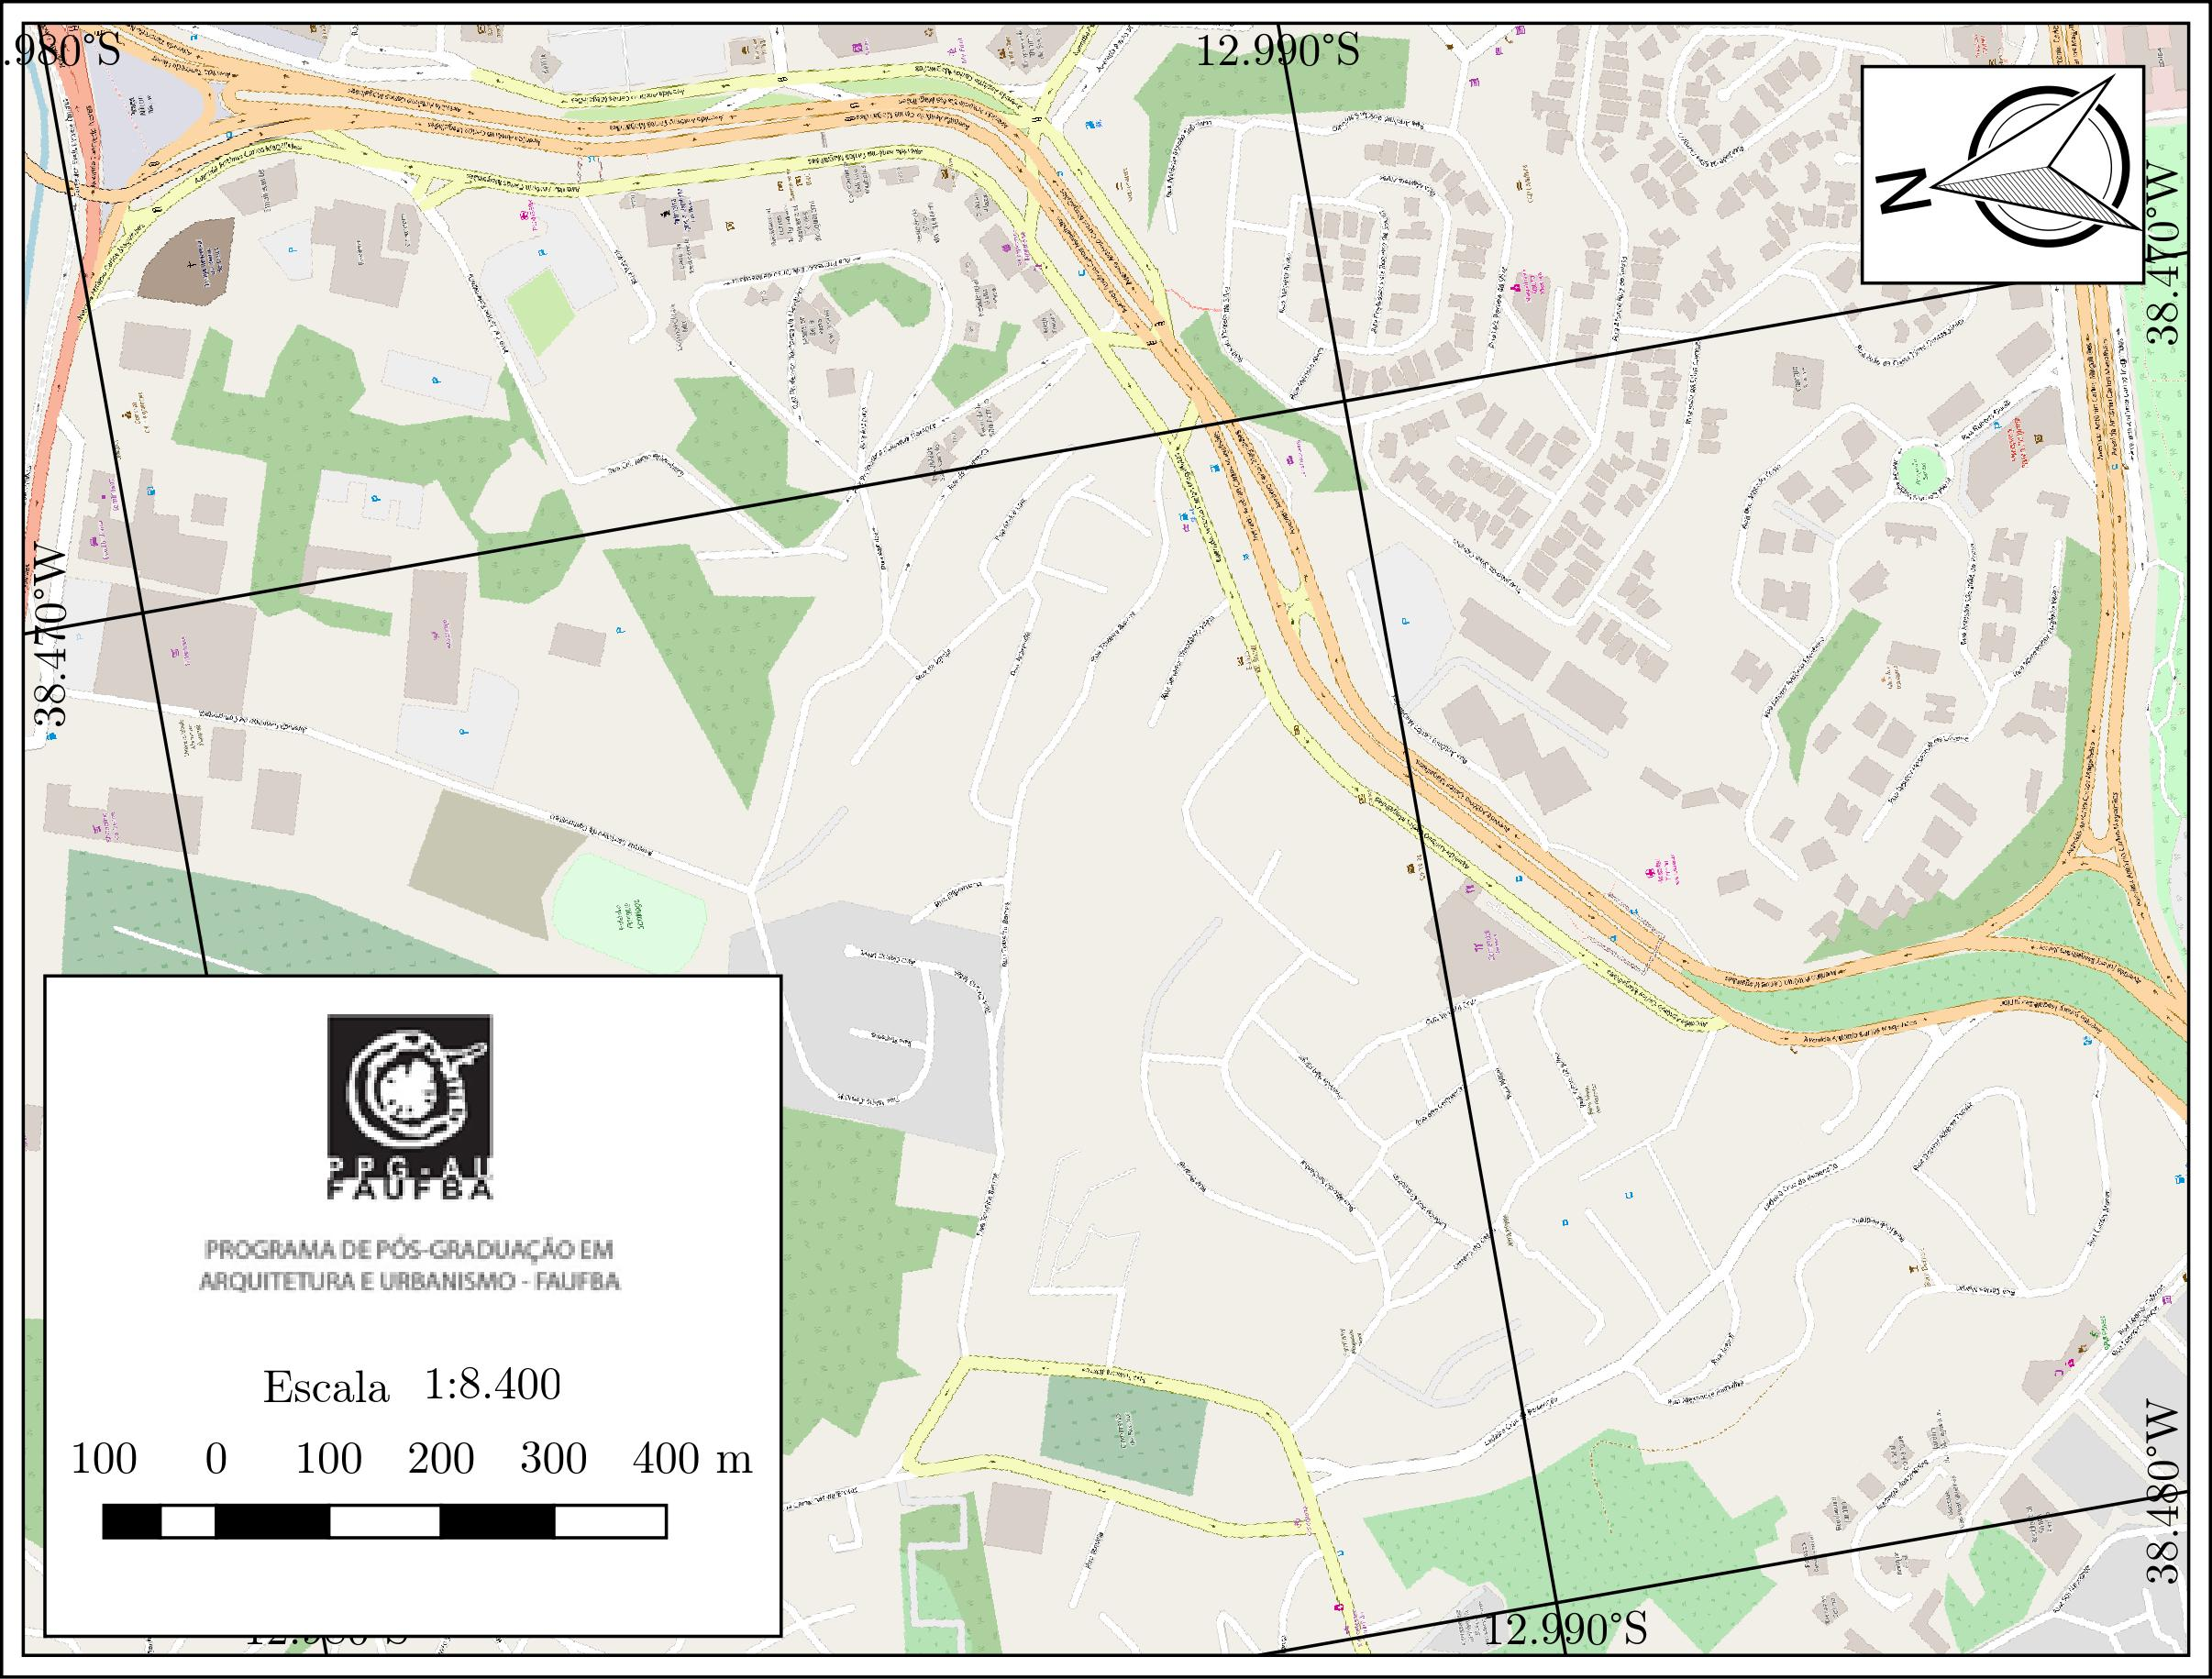
\includegraphics[width=0.8\textwidth]{3-cap2/complementos/mapas/georreferenciamento/campinas/campinas-2016.eps}{\footnotesize \par \textbf{Fonte:} Elaboração do autor com imagem do Open Street Maps. Respeitou-se o traçado de \citeonline{weyll_mappa_1851}. \par}
\caption{Representação cartográfica parcial da área de Campinas de Brotas e adjacências.}
\label{fig:campinas2016}
\end{sidewaysfigure}

No mapa de \citeonline{weyll_mappa_1851} (cf. \autoref{fig:campinas-1851}), vê-se nitidamente que o ``Engº'' marcado perto de ``Prambeé'' corresponde muito proximamente à descrição documental do Engenho Campina Grande, situado na baixada hoje correspondente à rua Santiago de Compostela. No cume logo abaixo do ``Engº'' no mapa, onde hoje se situam  o cemitério Jardim da Saudade e o Abrigo Salvador, tem início uma estrada que corresponde à atual rua Campinas de Brotas. À atual rua Teixeira Barros corresponde a antiga Estrada do Beijú; se o mapa de Weyll continuasse mais ao leste, seria possível observar como esta estrada se unia à Estrada das Armações no trecho onde se cruzam, hoje, as avenidas Paulo VI e Antônio Carlos Magalhães. Em 1845 se anunciava a venda, no Campina Grande, ``distante desta cidade tres quartos de legoa'', de ``capim bom e verde, já cortado, a 120 a arroba''\footnote{\textbf{O Mercantil}, 27 set. 1845, p. 4.}. Notícia de prisão efetuada em suas matas indica que o engenho Campina ainda existia enquanto tal em 1881\footnote{\textbf{O Monitor}, 10 jun. 1881, p. 1.}.

O inventário da solteirona Rosa Ladislau de Figueredo e Melo, filha do coronel João Ladislau de Figueredo e Melo e da senhora Francisca Joaquina Rodrigues falecida em 17 de abril de 1874, nos diz muito a respeito da fortuna da família. Segundo seu testamento escrito aos sessenta e seis anos em 30 de julho de 1860, suas irmãs Anna Ladislau do Amaral e Virgínia Ladislau de Figueredo e Melo, além de suas herdeiras, foram também nomeadas testamenteiras; além delas, foram nomeados herdeiros seus sobrinhos Evaristo Ladislau e Silva, Michelina Ladislau e Silva, Joanna Fausta Ladislau e Silva, Rita Ladislau do Amaral, Manoel Maria do Amaral (afilhado da falecida) e Anna Constança Ladislau e Silva. Na abertura do inventário Virgínia apresentou-se como inventariante e afirmou residir no engenho Campina Grande. Além dos costumeiros legados em rendas; de vários pequenos pagamentos ``em lembrança da minha pessoa'', que incluíram um a Leovigildo de Amorim Filgueiras (filho de Francisco Antonio Filgueiras, um dos muitos afilhados da falecida), outro a Laura Cypriano Barata (afilhada de crisma da falecida -- e filha do ``revoltoso'' Cypriano José de Almeida Barata \cite{morel_barata_2001}) e ainda outro a Januária Constança Labatut (também afilhada de crisma da falecida -- e filha do mercenário francês Pierre Labatut, heroi da guerra de independência na Bahia \cite{senado_anais_1851}); das tradicionais alforrias condicionadas a acompanhamentos a parentes por certo período; além disto tudo, parecia haver tantos bens a dividir que a falecida criou uma complexa divisão do monte por três, cabendo uma parte a cada uma de suas irmãs e a terceira a seu sobrinho Evaristo. A liquidação destes três montes foi operação igualmente complexa, pois cada item precisava ser descrito e avaliado para igualar os montes; neste processo apurou-se o valor do engenho Campina Grande em 18:000\$000 se considerada apenas a terra nua, e 31:006\$440 se considerado de porteira fechada; como parãmetro, observe-se que somente o palacete de Joaquim José de Oliveira (\autoref{fig:hospmil}, p. \pageref{fig:hospmil}) fora arrematado dois anos antes pela presidência da província por mais que o dobro do valor mais alto. Por fim, a partilha dos bens resultou em que o engenho Campina Grande foi compartilhado em condomĩnio pelos três quinhões\footnote{\textbf{BR BAAPB}, fundo Judiciário, seção Inventários, estante 5, caixa 1923, maço 2395, documento 2.}. No que diz respeito à parentela da falecida, o desembargador Manoel Maria do Amaral, filho de Anna Ladislau do Amaral, voltará à baila quando da análise da \textit{Cidade Balneária Amaralina} mais adiante.

\subsection{As fazendas Alagoa, Amaralina, Santa Cruz, Ubarana e Pituba: terras em disputa}\label{subsec:alagoaamaralina}

A história fundiária destas cinco fazendas cujo território pode ser visto de modo aproximado na \autoref{fig:armacaodalagoa} é inseparável, indissolúvel, indivisível. Limítrofes, integrantes do antigo morgado da Foz, seus antigos terrenos constituem, somados, a maior parte, senão a totalidade, dos atuais bairros de Amaralina, Pituba, Nordeste de Amaralina, Santa Cruz, Rio Vermelho, Itaigara, Iguatemi, Chapada do Rio Vermelho e Vale das Pedrinhas.

\subsubsection{Fazendas Alagoa e Amaralina: pesca e pecuária}

Um dos grandes imóveis saídos do morgado da Foz foi a \textit{fazenda Alagoa}, localizada onde hoje estão os bairros do Rio Vermelho e Amaralina.

Quando ainda integrava o morgado foram construídos dentro dela, em 1768, um tanque de captação de água, um engenho (há muito desaparecido) e uma ermida \cite[p.~118]{campos_alagoa_1942}. A ermida, transformada em capela dedicada a Nossa Senhora dos Mares, ainda existe nos dias de hoje, incorporada ao Quartel de Amaralina, localizado no mesmo sítio onde se erguia a casa-grande do engenho.

Já desmembrada do morgado, a fazenda Alagoa foi adquirida em 1797 por Alexandre Teotônio de Sousa, tenente-coronel de granadeiros da guarnição de Salvador; alguns seus herdeiros remotos venderam-na em 1854 a José Álvares do Amaral\footnote{O primeiro sobrenome desta personagem histórica encontra-se grafado como ``Alves'' ou ``Álvares'' a depender da fonte. Foi mantida a grafia tal como foi encontrada.} \cite[p.~118]{campos_alagoa_1942}, com os seguintes limites constantes do \textbf{Livro Eclesial de Registro de Terras da Freguesia de Brotas}:

\begin{citacao}
Terreno de José Alves do Amaral

Em obediência ao despacho do senhor Vice-Presidente Missias de Leão, de 29 de abril de 1859, exarei o seguinte registro:

José Alves do Amaral, tendo o domínio útil da fazenda ``Alagôa'', situada nesta freguesia das Brotas, vem apresentala ao registro das terras. Principia o limite da dita fazenda, do lado da Ubarana, de propriedade útil do Major Manoel de Barros Paim, por um marco de pedra de cantaria collocado em mil setecentos e oitenta e nove na costa do mar em direção NO 35gº no qual se acha gravada a seguinte inscripção '1789', e partindo dahi no rumo que mostra o dito marco a encontrar a valla mestra divisória que passa nos fundos da dita fazenda Ubarana, e seguindo pela dita valla a encontrar a área nativa que limita com a fazenda ``Pituba'', de propriedade do Visconde do Rio Vermelho, e acompanhando a dita cerca até encontrar a estrada que conduz para a Cruz da Redempção em Brotas, dividindo sempre por esta estrada com a fazenda ``Santa Cruz'', de propriedade de Antonio Joaquim da Silva e Abreu, até o lugar chamado ``tanque'', e seguindo dahi pela valla mestra a desembocar no rio Camorogipe, e por este abaixo até sua foz no mar pela parte da Mariquita, confrontando por este lado com terras pertencentes ao Mosteiro de São Bento, tendo a dita fazenda toda a frente para o mar, pela costa as terras da dita fazenda [\textit{ilegível}] do senhorio direto Thomas da Silva Paranhos. Cumpre declarar que os limites da mencionada fazenda se encontram em litígio com os [\textit{ilegível}] confrontantes da Ubarana e Santa Cruz. Bahia, quatro de abril de mil oitocentos e cincoenta e nove. José Álvares do Amaral. E nada mais continhão as declarações que me foram transmitidas. Brotas da Bahia, 3 de maio de 1859. Vigº Ernesto de Olivª Valle\footnote{\textbf{BR BAAPB}, fundo Colonial, série Registros de Terra, livro 4675, f. 36 verso e 37.}
\end{citacao}

No mapa de \citeonline{weyll_mappa_1851} (cf. Figura \autoref{fig:armacaodalagoa-1851}, p. \pageref{fig:armacaodalagoa-1851}) há a indicação de uma ``Armação da Lagoa'', compatível com os relatos da existência de uma armação de pesca nesta fazenda desde os idos do século XVIII \cite[p.~120-121]{campos_alagoa_1942}. O mesmo mapa mostra uma estrada que a liga ao largo de Brotas; trata-se, como visto na \autoref{subsubsec:brotasredencao} (p. \pageref{subsubsec:brotasredencao}), da \textit{estrada da Ubarana}, iniciada no que hoje é a ladeira da Cruz da Redenção e seguindo, de onde ela hoje termina, por um caminho que hoje não existe mais. Se seguirmos seu trajeto desde este largo até o mar e o compararmos com o trajeto de ruas atuais (cf. figura \autoref{fig:armacaodalagoa-hoje}, p. \pageref{fig:armacaodalagoa-hoje}), é plausível conceber alguns possíveis caminhos remanescentes da velha estrada da Ubarana\footnote{Com a base documental pesquisada até o momento é impossível descrever precisa e minuciosamente as ruas remanescentes desta estrada, e é possível mesmo que tal descrição documental sequer exista; a reconstituição desta estrada exigiria uma pesquisa \textit{in loco} com antigos moradores da Santa Cruz e do Nordeste de Amaralina para tentar recompor alguns traços perdidos desta estrada, profundamente modificada pela ocupação popular do território destes bairros, pelos loteamentos resultantes nos bairros de Amaralina e Pituba, e pela construção da avenida Juracy Magalhães e do Parque da Cidade.}

\begin{itemize}
\item Os dois caminhos saem do largo da Cruz da Redenção, descendo sua ladeira até o leito do rio Camorogipe, e o atravessam por meio de uma ponte (atualmente inexistente);
\item Uma primeira hipótese para um traçado remanescente desta estrada segue pela rua Onze de Novembro, ou Estrada da Santa Cruz, e daí pela rua do Futuro e pela avenida Nova República;
\item Uma segunda hipótese para o traçado corta caminho desde o leito do Camorogipe por dentro do atual Parque da Cidade, encontrando a avenida Nova República;
\item Da avenida Nova República o traçado segue encontrando-se com a rua Victorio Rossi para continuar pelo Beco da Cultura;
\item Uma linha imaginária ligaria o Beco da Cultura à rua Reinaldo de Matos, encontrando-se com a rua Cristóvão Ferreira;
\item Outra forma de ligar a avenida Nova República com a rua Cristóvão Ferreira seria sair da avenida para a rua Nova República, daí para a rua Valdomiro, depois para a travessa 20 de Junho, daí para as ruas do Areal e Ipanema, pela ruas Onze de Novembro e Francisco Sales até a rua dos Posseiros, e daí por uma linha imaginária até a rua Alto do Capim e, enfim, a rua Cristóvão Ferreira;
\item O caminho terminaria, por fim, na atual rua do Norte, ligada ao litoral por uma linha imaginária. 
\end{itemize}

É desta fazenda que deriva o loteamento, de final do século XIX, chamado \textit{Cidade Balneária Amaralina}, a ser detalhado no capítulo seguinte.

A compra da fazenda Alagoa foi fortemente contestada durante quase quarenta anos por Tomás da Silva Paranhos, comprador, como visto, do que restara do morgado da Foz \cite[p.~118]{campos_alagoa_1942}. José Álvares do Amaral seria ainda acusado por José Custodio da Silva, em 1881, de encontrar-se ``indevidamente'' na posse das fazendas Alagôa, Mariquita, Ubarana, Paciência e Santa Cruz; na qualidade de herdeiro e inventariante de Antonio Dias Soares, decidira prosseguir uma execução iniciada pelo inventariado e prosseguida por seu sogro, José Maria Frazão de Lima, contra Manuel Innocencio Pires de Figueiredo Camargo, herdeiro este último de Francisco Gomes de Sousa e Maria Magdalena de Sousa\footnote{\textbf{O Monitor}, ano VI, nº 151, 6 dez. 1881, p. 2.}. O processo, tal como noticiado, apresenta todas as características típicas do regime fundiário da época: títulos muito antigos, sucessões complexas de titulares, longuíssimas pendengas judiciais, gerações de titulares (não raro os ``notáveis'' de sua época) em litígio, indefinição dos limites de cada herdade, risco à posse de rendeiros, foreiros e inquilinos\dots José Álvares respondeu às acusações dizendo que comprou ``muito legalmente'' a fazenda Alagoa e entrou em sua posse por meio judicial em 1854; tudo isto seria fruto de uma dívida contraída em 1816 por antigos proprietários, em especial ``o sogro do sogro do sogro'' de José Custódio, que resultou numa penhora indevida e num \textit{imbroglio} fundiário que estaria sendo suscitado não por José Custódio, mas sim por ninguém menos que \textit{Rui Barbosa}, cujo interesse na questão seria apenas o de ``desmoralizar'' José Álvares frente aos eleitores do 2º distrito e frente a seus rendeiros, ``aos quaes aliás nunca persegui pelas rendas, que só paga um muito diminuto número d'ellas, que pode pagar''\footnote{\textbf{Gazeta de Notícias}, ano III, nº 209, 27 set. 1881, p. 2.}. Como se verá adiante (cf. \autoref{subsec:loteamentos}, p. \pageref{subsec:loteamentos}), José Custódio da Silva de fato entrou na posse de terrenos na fazenda Ubarana, não na Alagoa. Terminada a querela, diz um memorialista célebre que a fazenda teria sido rebatizada em 1912 pelo filho de José Álvares -- que depois de adulto adotou o mesmo nome do pai -- como fazenda \textit{Amaralina} \cite[p.~118]{campos_alagoa_1942}; porém, como se verá no capítulo seguinte, a documentação consultada dá a entender que já na década de 1890 vigiam para a área duas denominações distintas, \textit{Alagoa} e \textit{Amaralina}.

\begin{sidewaysfigure}[!htp]
\centering
\includegraphics[width=1\textwidth]{3-cap2/complementos/mapas/georreferenciamento/amaralina/armacaodalagoa-1851.eps}{\footnotesize \par \textbf{Fonte:} \citeonline{weyll_mappa_1851}. \par}
\label{fig:amaralina1851}
\caption{Representação cartográfica parcial das fazendas Alagoa, Amaralina, Santa Cruz, Ubarana e Pituba (1851)}
\end{sidewaysfigure}

\begin{sidewaysfigure}[!htp]
\centering
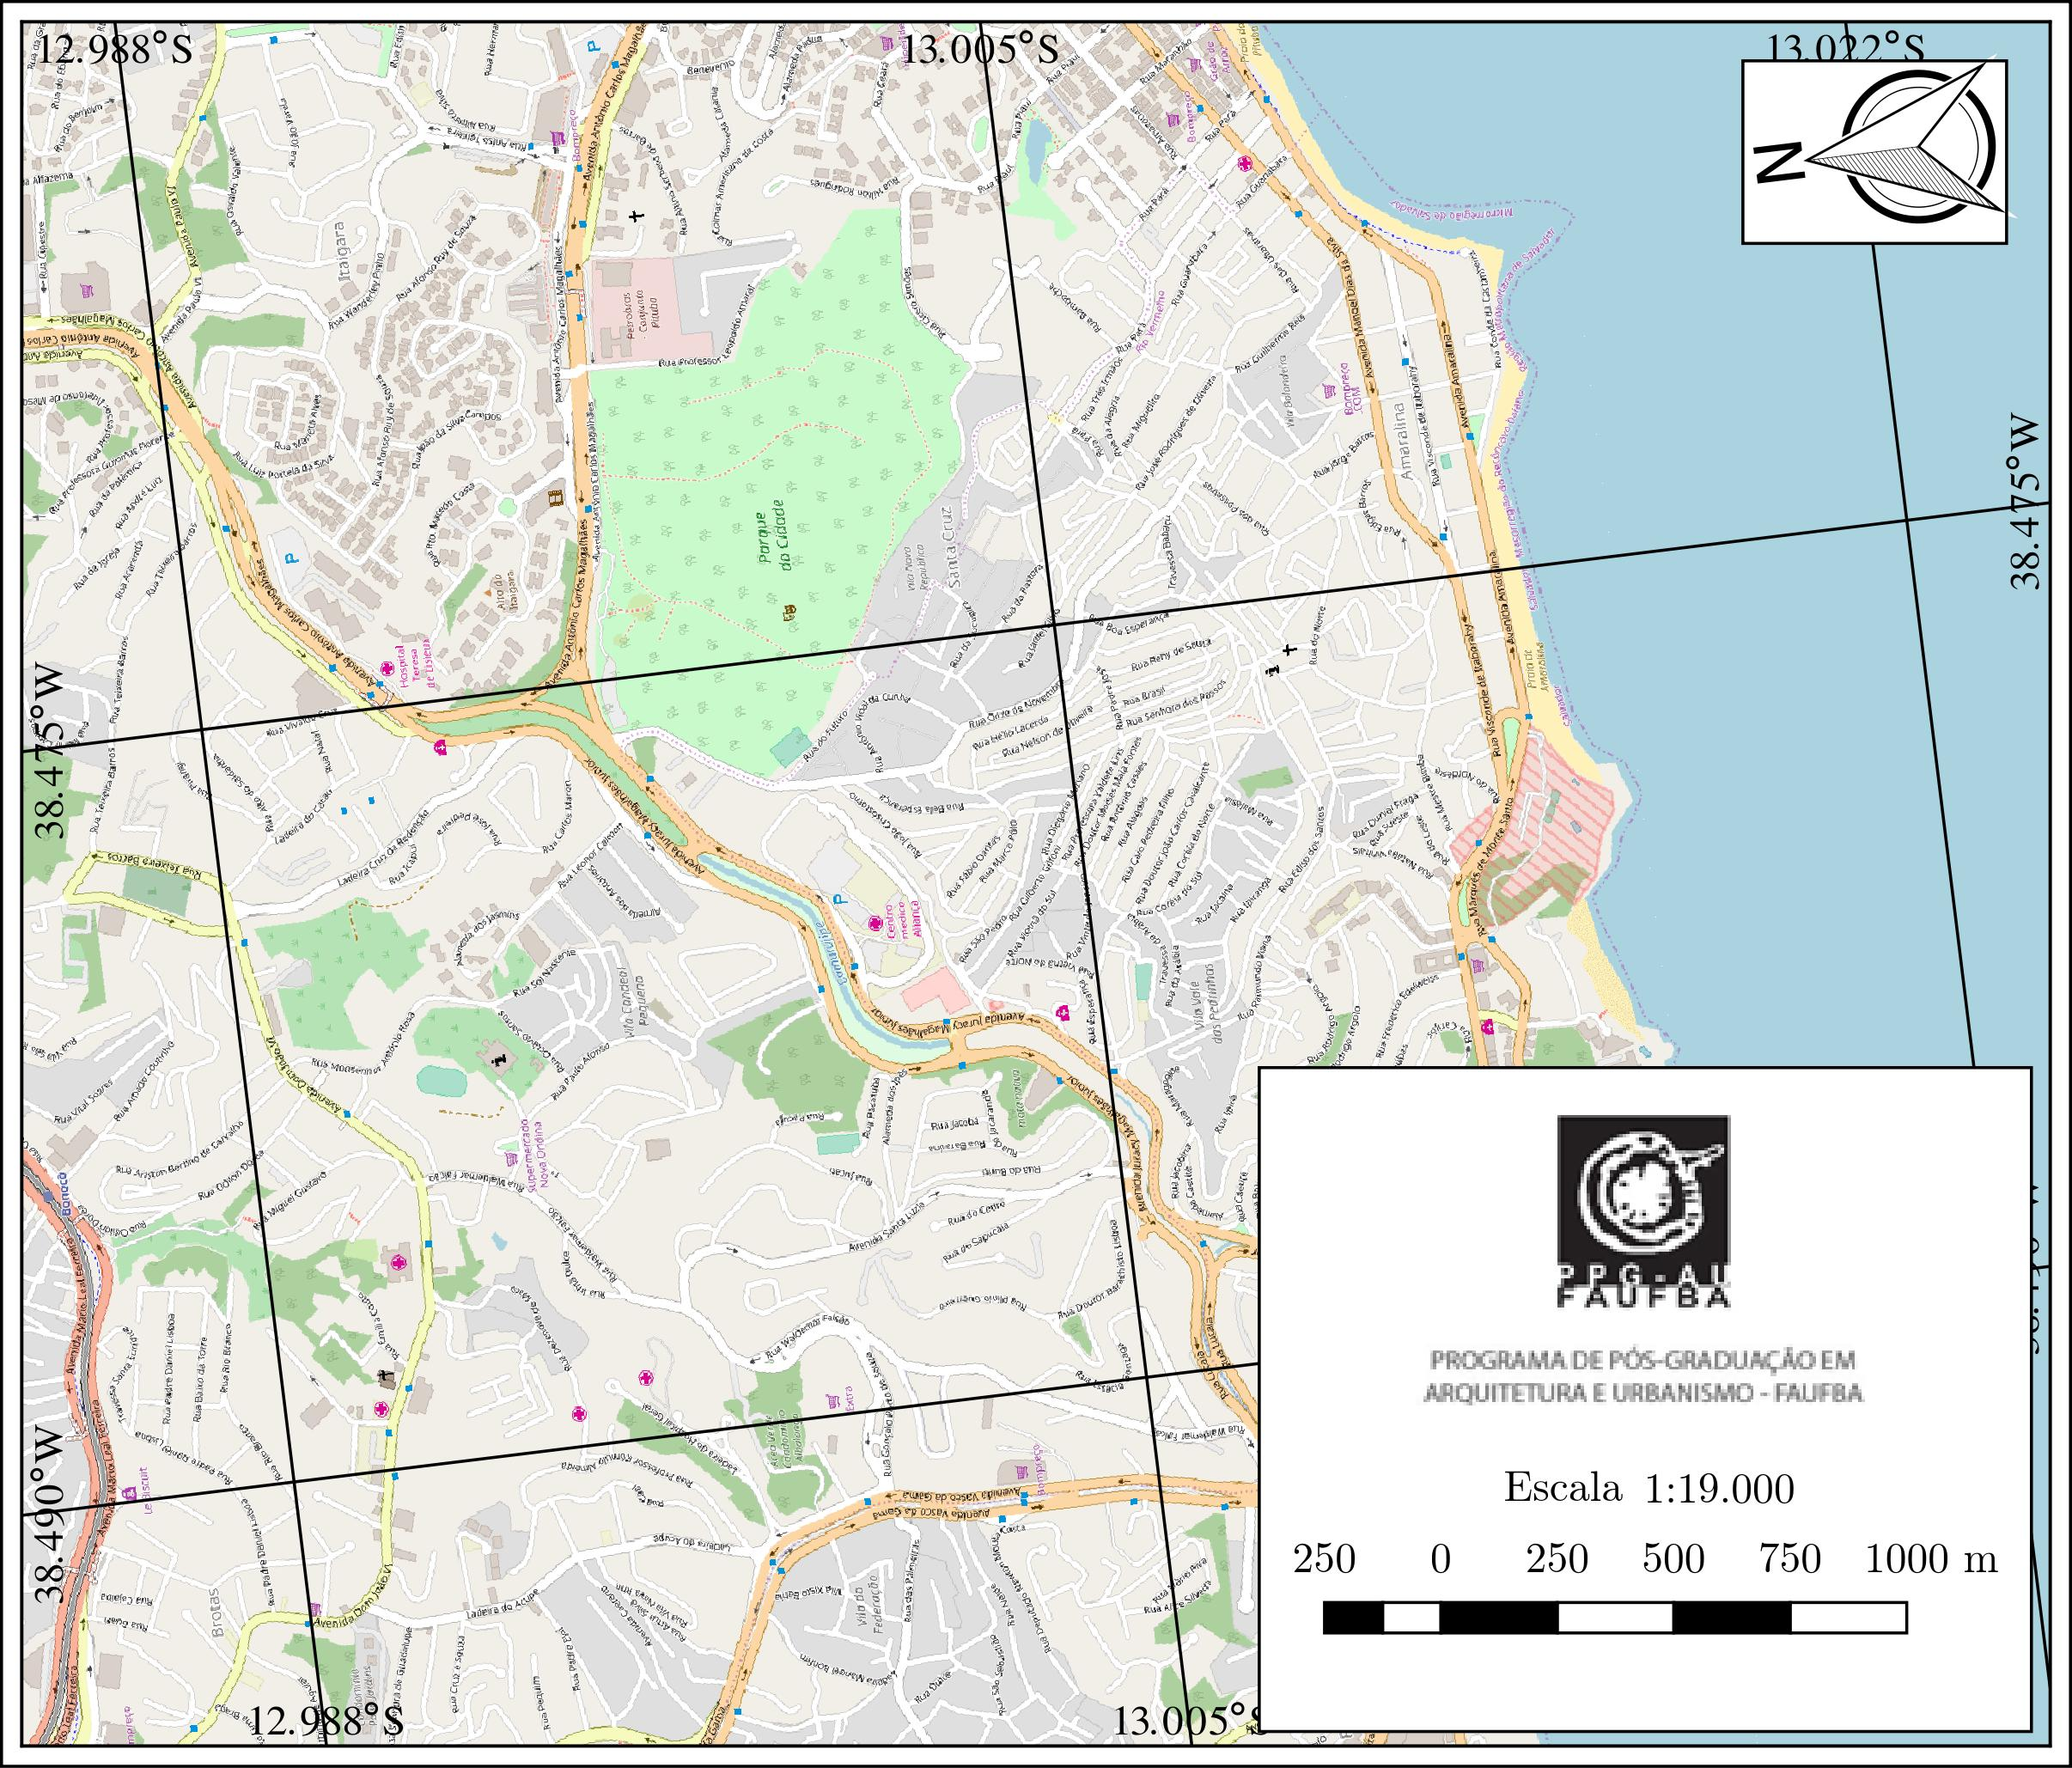
\includegraphics[width=1\textwidth]{3-cap2/complementos/mapas/georreferenciamento/amaralina/armacaodalagoa-2016.eps}{\footnotesize \par \textbf{Fonte:} Elaboração do autor com imagem do Open Street Maps. Respeitou-se o traçado de \citeonline{weyll_mappa_1851}. \par}
\caption{Representação cartográfica parcial da área entre a av. D. João VI e Amaralina, incluindo o Parque da Cidade e a av. Juracy Magalhães}
\label{fig:amaralina2016}
\end{sidewaysfigure}

\subsubsection{Fazenda Santa Cruz: área interna da localidade}

Menos célebre que a fazenda Alagoa, a \textit{fazenda Santa Cruz} é assim descrita no \textbf{Livro Eclesial de Registro de Terras da Freguesia de Brotas}:

\begin{citacao}
Fazenda de Antonio Joaquim da Silva e Abreu

Antonio Joaquim da Silva e Abreu possue na freguesia de Nossa Senhora de Brotas da Capital da Bahia uma fazenda denominada ``Santa Cruz'', em terrenos proprios, aqual limita-se pelo nascente com a fazenda Ubarana, pelo poente com o rio Camorogipe, pelo norte com a fazenda Pituba e pelo sul com o mesmo rio Camorogipe na povoação da Mariquita. Bahia e Freguesia de Brotas, vinte e sete de novembro de mil oitocentos e cincoenta e oito. Antonio Joaquim da Silva e Abreu. E nada mais continhão as declarações que me foram transmitidas. Brotas da Bahia, 27 de novembro de 1858. Vigº Ernesto de Olivª Valle\footnote{\textbf{BR BAAPB}, fundo Colonial, série Registros de Terra, livro 4675, f. 36 e 36 verso.}
\end{citacao}

Não foi possível encontrar quaisquer outras referências a esta fazenda na documentação pesquisada, mas no capítulo seguinte se verá como esta fazenda foi loteada ao final da Primeira República.

\subsubsection{Fazenda Ubarana: transição entre Amaralina e Pituba}

A \textit{fazenda Ubarana} é assim descrita no \textbf{Livro Eclesial de Registro de Terras da Freguesia de Brotas}, num registro que se encontra severamente atingido pela ação do tempo:

\begin{citacao}
A fazenda denominada Ubarana, sita na f[regue]sia de N[oss]a Senhora de [Bro]tas, da Capital [da] Bahia, divide-se pelos la[do]s do Sul com a[s fa]zendas Alagôa e Santa Cruz, a saber [ilegível]dindo do [ilegível] da Ubarana do lado do Sul em [li]nha recta a Pedra da Marca pelo caminh[o] que vae para Brotas, afindar-se no rio Camorogipe, a encontrar do lado norte com a [ilegível] nativa de antigas árvores que faz a [divi]za com a fazenda da Pituba, descendo athe vizinhanças do mar, [ilegível] desta os limites [ilegível] referida fazenda do [ilegível] [ilegível]. Brotas, vinte e oito de novembro de mil oitocentos e cincoenta e nove. Manuel [ilegível] de Barros Paim. E nada mais continhão as declarações que me foram transmitidas. Brotas da Bahia, 15 de janeiro de 1860. Vigº Ernesto de Olivª Valle\footnote{\textbf{BR BAAPB}, fundo Colonial, série Registros de Terra, livro 4675, f. 40.}
\end{citacao}

Difícil conhecer os limites desta fazenda, como se vê. Teria também desaparecido da memória coletiva, não fosse um resquício seu ainda ser encontrado no nome da atual \textit{rua das Ubaranas}, lindeira entre os atuais bairros da Pituba e Amaralina, que corre paralela à avenida Manoel Dias da Silva entre as ruas Pará e Vandick Badaró. O declarante desta averbação, cujo nome foi roído pelo tempo, pode ser encontrado em outros documentos: trata-se de \textit{Manuel Ignacio de Barros Paim}, agraciado com a Medalha da Guerra da Independência e lotado como capitão em 1854 \cite[p.~172]{masson_almanak_1854}. 

O mesmo \textbf{Livro Eclesial de Registro de Terras da Freguesia de Brotas} registra também a existência de terrenos de João da Cruz de Moraes na estrada da Ubarana\footnote{\textbf{BR BAAPB}, fundo Colonial, série Registros de Terra, livro 4675, f. 12 verso.}

O pouco encontrado a respeito da fazenda Ubarana na documentação pesquisada quase nada ilustra. Em 1882 a Recebedoria Geral da província, ao lançar os impostos predial, de indústrias e de profissões, fez menção a um ``becco da Ubarana'' na freguezia de Brotas\footnote{\textbf{Diário da Bahia}, ano XXVIII, nº 107, 14 maio 1882, p. 3}. Já em 1886 a mesma Recebedoria acusa apenas uma contribuinte da décima urbana na ``estrada da Ubarana'', Maria Antonia de Moraes, que deveria pagar 60\$000 de tributo\footnote{\textbf{Gazeta da Bahia}, ano VIII, nº 273, 14 dez. 1886, p. 2}. Só isto, nada mais.

A fazenda Ubarana retornará à baila mais adiante (cf. \autoref{subsec:loteamentos}, p. \pageref{subsec:loteamentos}) quando surgir, na Primeira República, uma proposta de seu loteamento por parte de José Custódio da Silva, sistematicamente negada pela municipalidade.

\subsubsection{Fazenda Pituba: história pregressa de um bairro}

A \textit{fazenda Pituba}, que incluía a \textit{Estrada do Pomar}, tem seus limites assim descritos no \textbf{Livro Eclesial de Registro de Terras da Freguesia de Brotas}:

\begin{citacao}
Terras da Exmª Viscondessa do Rio Vermelho

Limites da legoa de terra que pertence a Excellentíssima Viscondessa do Rio Vermelho e o condomino seo filho Barão do Rio Vermelho. Na freguesia de Nossa Senhora das Brotas está a fazenda denominada Pituba em um [ilegível] de terras que pertenceu a Casa da Excellentíssima Marquesa de Niza, hoje ao Capitão Thomas da Silva Paranhos, e [ilegível] de posse por escriptura de foro perpetuo para a Excellentíssima Viscondessa do Rio Vermelho e seu filho o Barão do Rio Vermelho. Tem por limites a dita fazenda ao sul divide com a fazenda Ubarana, ao norte com terras do Engenho Santo Antônio, ao nordeste com terras de São Bento, onde está a Armação do Gregório, e a leste com o mar. Bahia, quinze de julho de mil oitocentos e cincoenta e nove. Barão do Rio Vermelho. E nada mais continhão as declarações que me foram transmitidas. Brotas da Bahia, 15 de julho de 1859. Vigº Ernesto de Olivª Valle\footnote{\textbf{BR BAAPB}, fundo Colonial, série Registros de Terra, livro 4675, f. 38.}
\end{citacao}

Como se pode inferir dos limites constantes nos registros de terra, a povoação da Mariquita era o ponto de convergência, e portanto de conflito, entre os limites das fazendas Santa Cruz e Alagoa. A deterioração do registro da fazenda Ubarana dificulta compreender os limites entre ela e as demais fazendas, pois a descrição de alguns marcos foi corroída pela tinta.

Apesar da importância da fazenda, a Pituba era também sítio de uma pequena povoação composta principalmente por pescadores, registrada na documentação pesquisada ora como ``arraial'', ora como ``povoado''. Pouco se pode encontrar acerca desta povoação na documentação pesquisada, e a bibliografia consultada não o mencionou sequer uma vez senão como ponto notável. Tudo, literalmente tudo o que foi possível de encontrar vai a seguir.

Registrou-se em 1813 o naufrágio da galera \textit{Ingleza} na costa abrangida pela fazenda, do qual escapou toda a tripulação graças a socorro que lhes foi prestado desde a terra por ``escravos de huma armação de peixe, que tem naquelle sitio'' e de onde se salvou parte significativa da carga\footnote{\textbf{Idade D'Ouro do Brazil}, nª 45, 4 jun. 1813, p. 3}.

Em 1863 registrou-se José Rodrigues Setúbal como inspetor de quarteirão da Pituba \cite[p.~260]{masson_almanak_1863}, indicando que de algum modo havia a intenção de integrar este arrabalde à malha institucional urbana de Salvador. Em 1877 apenas três pessoas (Elesbão José da Paz, Estêvão Francisco dos Santos e Isidro José da Paz), todos de ``filiação desconhecida'', foram declarados aptos para o serviço no Exército e na Armada\footnote{\textbf{Correio da Bahia}, ano VII, nº 122, 22 ago. 1877, p. 3}. Naquele tempo, desconhecer pai e mãe era sinal de indigência.

Foi criada, em 23 de maio de 1885, uma ``cadeira mixta'' na ``povoação da Pituba''\cite[p.~126]{bahia_relatassleg_1886}; talvez seja isto o resultado dos esforços de Maria Dionizia Ribeiro Duarte, que em janeiro de 1878 peticionara sucessivas vezes à presidência da província pela criação desta cadeira e se oferecera como professora\footnote{\textbf{Correio da Bahia}, ano VII, nº 263, 12 fev. 1878, p. 2; \textbf{O Monitor}, ano II, nº 206, 8 fev 1878, p. 2}, ou de outros moradores inominados que fizeram o mesmo em agosto de 1877\footnote{\textbf{O Monitor}, ano II, nº 59, 10 ago. 1877, p. 1}; a \textit{mobilização} em prol da escola é o fato a destacar. O estabelecimento de uma escola no local indica não apenas a existência de crianças na localidade, mas igualmente uma povoação de algum modo numerosa ao ponto de exigir tal providência. A instalação desta escola deve ser vista também na sequência da transferência da escola de Brotas para as Pitangueiras em 1871, comentada na \autoref{subsubsec:pitangueiras} (p. \pageref{subsubsec:pitangueiras}) especialmente em função dos protestos dos moradores do largo de Brotas e adjacências; a Pituba não é próxima do largo de Brotas nem hoje, no tempo dos automóveis, mas parece ter havido o reconhecimento tácito por parte dos parlamentares baianos, com a instalação desta escola mista, de que a mudança teria realmente prejudicado os moradores dos sítios mais distantes da freguesia de Brotas.

A Pituba, de tão erma, encontrava-se desprovida inclusive de rondas policiais, criando enorme sensação de insegurança entre seus residentes e circunvizinhos. Basta recordar-se do caso do ``desordeiro'' da Cruz da Redenção atuante no início de 1889 mencionado na \autoref{subsubsec:brotasredencao} (p. \pageref{subsubsec:brotasredencao}) para constatá-lo: ali a Pituba não apenas parecia ser um lugar secundário para os moradores do largo de Brotas -- ele próprio distante e ``perigoso'' -- como também fica-se com a impressão, dada a ausência, na documentação pesquisada e na bibliografia consultada, de protestos semelhantes vindos de moradores da localidade, de que ``desordeiros'' semelhantes tinham livre tráfego no lugar enquanto não molestassem vizinhanças mais ``respeitáveis''.

\subsection{Várzea de Santo Antônio e as Armações: últimas fronteiras de Brotas}

Conquanto seja comum pensar que a freguesia de Brotas terminava na Pituba, mais especificamente em algum ponto entre as armações do Saraiva e do Gregório, as terras nela compreendidas iam mais além, como se pode ver no \textbf{Livro Eclesial de Registro de Terras da Freguesia de Brotas}. Um primeiro indício são as terras registradas em nome do comendador Francisco Lourenço da Costa Lima:

\begin{citacao}
O Commendador Francisco Lourenço da Costa Lima possue na freguesia de Brotas huma sorte de terras foreiras ao Convento de São Bento desta cidade, a qual tem por limites os seguintes: tem princípio pelo lado do sul da pedra de marco da armação Saraiva, que divide as terras do dito convento de São Bento com as da Marqueza de Niza, seguindo linha recta para o norte até o rio das Pedras onde finda, pelo lado do oeste divide com as terras do mesmo convento, seguindo riacho chamado Estiva até a estrada do Cabula; pelo leste divide-se sempre pela pancada do mar. Bahia e Armação, treze de julho de mil oitocentos e cincoenta e nove. Francisco Lourenço da Costa Lima. E nada mais continhão as ditas declarações. Brotas da Bª, 14 de julho de 1859. Vigº Ernesto de Olivª Valle\footnote{\textbf{BR BAAPB}, fundo Colonial, série Registros de Terra, livro 4675, f. 37 verso.}.
\end{citacao}

Outro indício são as terras registradas em nome de Maria Joana da Conceição Simões, Viscondessa do Rio Vermelho \cite[p.~693]{zuquete_nobreza_1989}:

\begin{citacao}
Limites do foro perpétuo pertencente à Excelentíssima Viscondessa do Rio Vermelho como herdeira do seu fallecido filho o Capitão Tristão da Cunha e Meneses e condomina sua filha Judith Constança da Cunha e Meneses Balthazar da Silveira. Engenho Santo Antonio sito na freguesia das Brotas, está collocado em terreno foreiro que pertenceu à Casa da Excelentíssima Marqueza da Niza, hoje do Capitão Thomaz da Silva Paranhos, cujo terreno estão [\textit{ilegível}] por escriptura de foro perpetuo à Excelentíssima Viscondessa do Rio Vermelho como herdeira de seu filho e Judith Constança da Cunha Balthazar da Silveira, e [\textit{ilegível}] [\textit{ilegível}] o Tentente Coronel José Balthazar da Silveira, por partilha fraterna. Tem tres frentes a saber pela estrada real que vai para as Armaçoens e Itapoan [\textit{ilegível}] as ditas terras da ponte denominada do Rio Camorogipe seguindo por um antigo [\textit{ilegível}] da frente em direção a leste, a dividir com o outro foro denominado da Costa do mar, [\textit{ilegível}] e ao norte com a estrada real do Cabulla. Bahia, quinze de julho de mil oitocentos e cincoenta e nove. Viscondessa do Rio Vermelho. José Balthazar da Silveira. Judith Constança da Cunha Balthazar da Silveira. E nada mais continhão as declaraçoens que me forão transmitidas. Brotas da Bahia, 18 de julho de 1859. Vigº Ernesto de Olivª Valle\footnote{\textbf{BR BAAPB}, fundo Colonial, série Registros de Terra, livro 4675, f. 38 verso.}.
\end{citacao}

A viscondessa registrou em seu nome e de seus herdeiros terras que haviam pertencido a seu finado marido, Manuel Ignácio da Cunha e Meneses (1779-1850), criado por decreto imperial em 17 de desembro de 1830 como \textit{visconde do Rio Vermelho}. Veterano da guerra pela independência na Bahia, quando comandou na patente de tenente-coronel um batalhão e tornou-se bastante próximo do coronel João Ladislau de Figueredo e Melo, seu vizinho de herdades, o visconde foi vice-presidente da província da Bahia (1835) e senador do Império (1829-1850) \cite[p.~404]{vasconcellos_arnobili_1918}. Sua riqueza vinha da pesca da baleia, que dominava na extensão que ia da Pituba (fazenda de sua propriedade) até Itapuã; uma fonte bibliográfica não muito precisa diz ter vivido o visconde numa casa senhorial com capela, transformada, mais de século depois, no que diz esta fonte ter sido a sede do Aeroclube da Bahia \cite{riserio_histba_2004}\footnote{Antonio Risério, mais antropólogo que historiador, situa o imóvel ``na Armação do Saraiva, ali pelo Carimbamba'' \cite{riserio_histba_2004}; ora, \textit{Carimbamba} corresponde aproximadamente ao trecho da orla atlântica soteropolitana compreendido entre a foz do rio das Pedras e a praia de Patamares, enquanto o lugar onde se situava a antiga armação foi também conhecido como \textit{Chega Negro} por força, segundo a tradição local, do tráfico ilegal de escravos que ali operava à solta.}.

O engenho Santo Antônio aqui referido é o mesmo que \citeonline{ott_engenhos_1996} dá como pertencente a Itapuã. No que diz respeito à mencionada estrada do Cabula, embora não haja referências mais seguras é factível a hipótese de que se trate de uma denominação antiga do caminho formado pelas atuais estrada do Saboeiro e avenida Silveira Martins. Este mesmo engenho, segundo o que se percebeu da documentação pesquisada, deu origem ao topônimo \textit{várzea de Santo Antônio} ou \textit{baixa de Santo Antônio} encontrado várias vezes no curso da pesquisa.

Chega-se com estas duas herdades a um ponto tão deserto da freguesia de Brotas que, salvo pelas menções escriturais, não foi possível encontrar qualquer outra notícia, menção, anúncio, registro de habitantes ou de estabelecimentos profissionais, seja na documentação pesquisada, seja na bibliografia consultada. Melhor dizendo: o que há são \textit{notícias policiais} e um ou outro \textit{expediente burocrático}, todos mal ocultando em suas entrelinhas a \textit{miséria} dos habitantes da localidade. Dois casos ilustram a questão.

Em 1876 noticiava-se que ``um indivíduo de nome Bernardo de tal'' fora encontrado enforcado num pé de massaranduba\footnote{\textbf{O Monitor}, ano I, 28 nov. 1876, nº 147, p. 1}; o subdelegado do Rio Vermelho, ao que tudo indica, assumiu de pronto a hipótese de suicídio e, tendo levantado o desaparecimento deste ``indivíduo'' desde três dias antes da localização de seu cadáver, deixou tudo por isto mesmo. Sequer a um nome na imprensa o pobre ``suicida'' teve direito, que dirá uma investigação adequada das circunstâncias de sua morte\dots tão distante foi a morte de ``Bernardo de tal'' para os soteropolitanos de seu tempo que mesmo a várzea de Santo Antônio, lugar onde se lhe encontraram os restos, foi confundida com a Pituba!

Em 1877 apenas cinco pessoas (Antonio José dos Santos, Epiphanio José Nunes, José Romão dos Martyres, Lauriano Francisco Alves e Sergio Pereira da Assumpção), todos de ``filiação desconhecida'', foram declarados aptos para o serviço no Exército e na Armada\footnote{\textbf{Correio da Bahia}, ano VII, nº 122, 22 ago. 1877, p. 3}. Naquele tempo, desconhecer mesmo pai e mãe nos anos da mocidade era sinal de \textit{extrema} pobreza e desamparo. Como teriam vivido estes jovens? Seriam pescadores, vinculados às velhas armações do Gregório ou do Saraiva? Agricultores, posseiros nas terras da casa do Rio Vermelho? Escravos? Libertos? Impossível saber. Como que condenados pela sua condição à insignificância histórica, restou deles apenas este único rastro.

\subsection{Delimitação aproximada da freguesia de Brotas}

Com todas as informações anteriores, a fronteira do distrito de Brotas fica mais precisamente delimitada que na descrição reproduzida por \citeauthoronline{NASCIMENTO2007}. Retornemos a ela:

\begin{citacao}
A freguesia de Nossa Senhora de Brotas foi criada pelo arcebispo D. Sebastião Monteiro da Vide, em 1718, sendo a seguinte sua demarcação extrema com outras freguesias, no século XIX: com Santo Antônio Além do Carmo pela Estrada Nova, começando pela roça do comendador Barros Reis, vindo até a Fonte Nova no Dique, onde fazia diferentes limites com Santana e São Pedro. Daí, pela estrada Dois de Julho, seguia até a ponta da Mariquita, de onde se espraiava costeando a lagoa da Pituba, até Armação e o Rio das Pedras, quando se dividia com a freguesia de Itapuã, suburbana da cidade. Seguia a freguesia de Brotas até o Engenho da Bolandeira, onde novamente fazia divisa com Itapuã e com a freguesia de Santo Antônio Além do Carmo. Limitava-se com a Vitória na Mariquita \cite[p.~58]{NASCIMENTO2007}.
\end{citacao}

Compare-se-a, agora, com a descrição a seguir, onde pontos notáveis do século XIX serão empregues junto a outros da atualidade para facilitar a visualização:

\begin{itemize}
\item Adota-se arbitrariamente como marco inicial, entre aqueles que se verificou integrarem o território da freguesia, o pé da Ladeira dos Galés, onde Brotas fazia fronteira com a freguesia de Sant'Anna.
\item Partindo deste ponto, a freguesia de Brotas margeia o Dique do Tororó pelo lado do Engenho Velho de Brotas, limitando-se com a freguesia de Sant'Anna até o ponto onde o dique dá origem ao rio Lucaia.
\item A partir daí a fronteira de Brotas com a freguesia da Vitória margeia o rio Lucaia até sua foz, no Rio Vermelho.
\item Daí em diante Brotas limita-se com o mar até a foz do rio das Pedras, na Boca do Rio, que separa Brotas da freguesia suburbana de Itapuã. A fronteira segue margeando o rio das Pedras da foz até o riacho Estiva.
\item Não foi possível localizar o riacho Estiva na documentação pesquisada ou na bibliografia consultada. Sabe-se, entretanto, que atualmente o rio das Pedras é formado pela confluência entre os rios Saboeiro, Cascão, Cachoeirinha e Pituaçu \cite[p.~175]{santos_aguas_2010}; com isto, e com a informação de que os limites das terras de Francisco Lourenço da Costa Lima corriam deste riacho até a estrada do Cabula, é factível, ao menos em termos aproximativos, situar estes limites como sendo compostos pelo rio das Pedras, pelo rio Saboeiro e pelas atuais avenidas Edgard Santos e Silveira Martins, onde a freguesia de Brotas limitava-se com as freguesias do Santo Antônio e de Itapuã.
\item Como o leito do Camarajipe àquela altura correspondia ao leito do rio Pernambués, que corre rente à atual avenida Luiz Eduardo Magalhães, é factível traçar uma linha que vá do rio Saboeiro até o rio Pernambués e seguir seu traçado rumo à região onde se situam atualmente a rodoviária de Salvador e o Shopping da Bahia. Em todo este traçado Brotas confronta-se com a freguesia do Santo Antônio.
\item A partir daí é possível, como se vê em \citeonline{weyll_mappa_1851}, margear o Camarajipe até que ele encontre com a rua da Vala na altura da atual rótula do Abacaxi, novamente confrontando Brotas e Santo Antônio.
\item A rua da Vala limita as freguesias de Brotas e Santo Antônio até o ponto onde se encontra com a atual rua Djalma Dutra.
\item Deste ponto em diante a rua Djalma Dutra segue delimitando as freguesias de Brotas e Santo Antônio até encerrar-se no pé da ladeira dos Galés, ponto inicial desta descrição.
\end{itemize}

Com estas terras fechava-se o perímetro da freguesia de Brotas. Iniciada próxima ao centro de Salvador, a freguesia viria a terminar mais de dez quilômetros depois, lá onde não mais havia qualquer sinal de urbanização.

\subsection{Evolução comparada da urbanização: o Livro de Registro de Terras (1858-1862) e as décimas urbanas (1886-1891)}

Se todo o panorama traçado até o momento confirma a impressão inicial, de uma freguesia rural em processo lento de urbanização, confirmam-na mais ainda uma lista de imóveis cadastrados para pagamento das décimas urbanas do quinquênio 1886-1891 apresentada pela Recebedoria Provincial da Bahia na \textbf{Gazeta da Bahia}\footnote{\textbf{Gazeta da Bahia}, ano VIII, nº 273, 14 dez. 1886, p. 2}:

\begin{table}[!htp]
\centering
\IBGEtab{
\caption{Logradouros cadastrados (1886-1891)}\label{tab:decurb1886-1891}}
{ \begin{tabular}{lll}
\toprule
Logradouro				& Total	& \% da freguesia\\
\midrule \midrule
(sem nome)				& 25				& 8,36\%		\\
Estrada da Quinta das Beatas		& 8				& 2,68\%		\\
Quinta das Beatas			& 6				& 2,01\%		\\
Matatu Pequeno				& 24				& 8,03\%		\\
Matatu Grande				& 38				& 12,71\%	\\
Estrada para a Casa da Pólvora		& 4				& 1,34\%		\\
Estrada do Engenho Velho		& 8				& 2,68\%		\\
Boa Vista				& 8				& 2,68\%		\\
Ladeira da Boa Vista			& 2				& 0,67\%		\\
Ladeira do Acu				& 2				& 0,67\%		\\
Estrada do Acu				& 13				& 4,35\%		\\
Largo do Acu				& 2				& 0,67\%		\\
Estrada do Acu para a 2 de Julho	& 5				& 1,67\%		\\
Estrada de Brotas			& 15				& 5,02\%		\\
Estrada da Cruz das Almas		& 14				& 4,68\%		\\
Largo de Brotas				& 39				& 13,04\%	\\
Estrada para a Cruz da Redenção		& 4				& 1,34\%		\\
Largo da Cruz da Redenção		& 4				& 1,34\%		\\
Campina					& 2				& 0,67\%		\\
Candeal					& 3				& 1,00\%		\\
Mariquita				& 65				& 21,74\%	\\
Estrada do Sangradouro para o Matatu	& 11				& 3,68\%		\\
Alto do Sangradouro			& 4				& 1,34\%		\\
Estrada da Ubarana			& 1				& 0,33\%		\\
Pomar					& 5				& 1,67\%		\\
Lagoa					& 1				& 0,33\%		\\
Estrada para a Armação			& 7				& 2,34\%		\\
Várzea de Santo Antonio			& 1				& 0,33\%		\\
Armação					& 3				& 1,00\%		\\
\midrule
TOTAL					& 324				& 100,00\%	\\
\bottomrule
\end{tabular}}
{\fonte{\textbf{Gazeta da Bahia}, ano VIII, nº 273, 14 dez. 1886, p. 2.}}
\end{table}

\begin{itemize}
\item A povoação da Mariquita concentrava ao final do século XIX o maior número de imóveis da freguesia, seguida de perto pela soma dos dois Matatus e depois pelo Largo de Brotas; superou em muito o número de imóveis da localidade mais povoada de Brotas em meados do século XIX, o Matatu.
\item Mesmo com a proibição legal à posse ou propriedade de bens de raiz por escravos\footnote{Já no século XVII o Título LXX das Ordenações Filipinas proibia escravos de ``viver por si'', ou seja, de morar em alguma casa por conta própria; a Lei Provincial nº 9, de 13 de maio de 1835, na esteira da Revolta dos Malês, proibiu aos africanos a aquisição de bens de raiz, e também o aluguel ou arrendamento de casas a africanos que não apresentassem autorização especial para este fim, dada por juiz de paz; tais proibições foram relaxando e caindo em desuso à medida em que avançava e recrudescia a luta abolicionista, em especial a partir da década de 1870.}, nota-se o arrolamento, ainda que minoritário, de ``africanos'' e ``creoulos'' como contribuintes da décima urbana;
\item Tanto na Lagoa quanto na Várzea de Santo Antônio os únicos imóveis pertencem a latifundiários (respectivamente, José Álvares do Amaral e a Baronesa do Rio Vermelho);
\item Os dois imóveis da Campina, muito provavelmente as fazendas Campina Grande e Campina Pequena, já não pertencem mais aos Ladislau, e sim ao desembargador Manuel Maria do Amaral;
\item Todos os quatro imóveis da Boa Vista pertencem ao taberneiro Aprígio Monteiro de Carvalho, e a situação da área formada pela Estrada do Engenho Velho, Boa Vista e Ladeira da Boa Vista dá a entender que os imóveis ali presentes eram de grande tamanho.
\end{itemize}

Quando comparada esta lista com o conteúdo do \textbf{Livro Eclesial de Registro de Terras da Freguesia de Brotas}, há ainda outros pontos a destacar:

\begin{table}
\centering
\IBGEtab{ \caption{Comparativo entre dados imobiliários de 1858-1862 e 1886-1891}
\label{tab:compara-brotas} }
{
\begin{tabular}{m{4cm}llll}
\toprule
Localidade	& Imóveis (1858-1862)	& Imóveis (1886-1891)	& Variação	& Variação (\%) \\
\midrule \midrule
Acupe	& 17	& 22	& 5	& 29,41\% \\
Alagôa	& 1	& 1	& 0	& 0,00\% \\
Armação	& 1	& 3	& 9	& 900,00\% \\
Beiju / Estrada das Armações	& 2	& 7	& -2	& -100,00\% \\
Brotas	& 1	& 1	& 0	& 0,00\% \\
Bulhões	& 1	& 0	& -1	& -100,00\% \\
Campinas	& 7	& 2	& -5	& -71,43\% \\
Candeal	& 3	& 3	& 0	& 0,00\% \\
Cruz da Redenção	& 4	& 8	& 4	& 100,00\% \\
Cruz das Almas / Estrada Brotas/Rio Vermelho	& 7	& 14	& 7	& 100,00\% \\
Engenho Velho / Boa Vista	& 6	& 18	& 12	& 200,00\% \\
Estrada da União	& 2	& 0	& -2	& -100,00\% \\
Estrada de Brotas	& 13	& 15	& 2	& 15,38\% \\
Largo de Brotas	& 5	& 39	& 34	& 680,00\% \\
Lucaia	& 1	& 0	& -1	& -100,00\% \\
Mariquita	& 0	& 65	& 65	& 6500,00\% \\
Matatu	& 50	& 66	& 16	& 32,00\% \\
Pitangueiras	& 2	& 0	& -2	& -100,00\% \\
Pituba	& 1	& 0	& -1	& -100,00\% \\
Pomar	& 0	& 5	& 5	& 500,00\% \\
Quinta das Beatas	& 3	& 14	& 11	& 366,67\% \\
Rua da Vala	& 1	& 0	& -1	& -100,00\% \\
Sangradouro	& 7	& 15	& 8	& 114,29\% \\
Santa Cruz	& 1	& 0	& -1	& -100,00\% \\
(sem nome)	& 0	& 25	& 25	& 2500,00\% \\
Torre	& 2	& 0	& -2	& -100,00\% \\
Ubarana	& 2	& 2	& 0	& 0,00\% \\
Várzea / Engenho de Santo Antônio	& 1	& 1	& 0	& 0,00\% \\
\midrule
TOTAL	& 136	& 326	& 190	& 58,28\% \\
\bottomrule
\end{tabular} 
}
{\fonte{Elaboração do autor, com base em dados do \textbf{Livro Eclesial de Registro de Terras da Freguesia de Brotas} (\textbf{BR BAAPB}, fundo Colonial, série Registros de Terra, livro 4675) e da lista de imóveis cadastrados para pagamento das décimas urbanas do quinquênio 1886-1891 apresentada pela Recebedoria Provincial da Bahia (\textbf{Gazeta da Bahia}, ano VIII, nº 273, 14 dez. 1886, p. 2).}}
\end{table}

\begin{itemize}
\item A \autoref{tab:compara-brotas} apresenta vários ``zeros'', que se podem atribuir, além dos problemas tradicionais nos levantamentos e estatísticas oficiais do período (``Beiju''), ao fato de que várias localidades desapareceram (``Bulhões''), foram criadas (``sem nome'', ``Pomar'') ou tiveram seu nome alterado entre um levantamento e outro.
\item Nota-se forte tendência à desconcentração imobiliária verificada no Matatu a partir do \textbf{Livro Eclesial de Registro de Terras da Freguesia de Brotas} segue como regra, aprofundando-se inclusive;
\item A mesma Michelina Ladislau e Silva que consta no \textbf{Livro Eclesial de Registro de Terras da Freguesia de Brotas} como uma das proprietárias da fazenda Campina Pequena ressurge aqui, como ``Miquelina Ladislau e Silva'', dividindo a propriedade de um imóvel na ``Ladeira do Acú'';
\end{itemize}



